\documentclass[twoside]{book}

% Packages required by doxygen
\usepackage{fixltx2e}
\usepackage{calc}
\usepackage{doxygen}
\usepackage{graphicx}
\usepackage[utf8]{inputenc}
\usepackage{makeidx}
\usepackage{multicol}
\usepackage{multirow}
\PassOptionsToPackage{warn}{textcomp}
\usepackage{textcomp}
\usepackage[nointegrals]{wasysym}
\usepackage[table]{xcolor}

% Font selection
\usepackage[T1]{fontenc}
\usepackage{mathptmx}
\usepackage[scaled=.90]{helvet}
\usepackage{courier}
\usepackage{amssymb}
\usepackage{sectsty}
\renewcommand{\familydefault}{\sfdefault}
\allsectionsfont{%
  \fontseries{bc}\selectfont%
  \color{darkgray}%
}
\renewcommand{\DoxyLabelFont}{%
  \fontseries{bc}\selectfont%
  \color{darkgray}%
}
\newcommand{\+}{\discretionary{\mbox{\scriptsize$\hookleftarrow$}}{}{}}

% Page & text layout
\usepackage{geometry}
\geometry{%
  a4paper,%
  top=2.5cm,%
  bottom=2.5cm,%
  left=2.5cm,%
  right=2.5cm%
}
\tolerance=750
\hfuzz=15pt
\hbadness=750
\setlength{\emergencystretch}{15pt}
\setlength{\parindent}{0cm}
\setlength{\parskip}{0.2cm}
\makeatletter
\renewcommand{\paragraph}{%
  \@startsection{paragraph}{4}{0ex}{-1.0ex}{1.0ex}{%
    \normalfont\normalsize\bfseries\SS@parafont%
  }%
}
\renewcommand{\subparagraph}{%
  \@startsection{subparagraph}{5}{0ex}{-1.0ex}{1.0ex}{%
    \normalfont\normalsize\bfseries\SS@subparafont%
  }%
}
\makeatother

% Headers & footers
\usepackage{fancyhdr}
\pagestyle{fancyplain}
\fancyhead[LE]{\fancyplain{}{\bfseries\thepage}}
\fancyhead[CE]{\fancyplain{}{}}
\fancyhead[RE]{\fancyplain{}{\bfseries\leftmark}}
\fancyhead[LO]{\fancyplain{}{\bfseries\rightmark}}
\fancyhead[CO]{\fancyplain{}{}}
\fancyhead[RO]{\fancyplain{}{\bfseries\thepage}}
\fancyfoot[LE]{\fancyplain{}{}}
\fancyfoot[CE]{\fancyplain{}{}}
\fancyfoot[RE]{\fancyplain{}{\bfseries\scriptsize Generated on Sat Aug 22 2015 14\+:51\+:28 for Cobra\+Lang by Doxygen }}
\fancyfoot[LO]{\fancyplain{}{\bfseries\scriptsize Generated on Sat Aug 22 2015 14\+:51\+:28 for Cobra\+Lang by Doxygen }}
\fancyfoot[CO]{\fancyplain{}{}}
\fancyfoot[RO]{\fancyplain{}{}}
\renewcommand{\footrulewidth}{0.4pt}
\renewcommand{\chaptermark}[1]{%
  \markboth{#1}{}%
}
\renewcommand{\sectionmark}[1]{%
  \markright{\thesection\ #1}%
}

% Indices & bibliography
\usepackage{natbib}
\usepackage[titles]{tocloft}
\setcounter{tocdepth}{3}
\setcounter{secnumdepth}{5}
\makeindex

% Hyperlinks (required, but should be loaded last)
\usepackage{ifpdf}
\ifpdf
  \usepackage[pdftex,pagebackref=true]{hyperref}
\else
  \usepackage[ps2pdf,pagebackref=true]{hyperref}
\fi
\hypersetup{%
  colorlinks=true,%
  linkcolor=blue,%
  citecolor=blue,%
  unicode%
}

% Custom commands
\newcommand{\clearemptydoublepage}{%
  \newpage{\pagestyle{empty}\cleardoublepage}%
}


%===== C O N T E N T S =====

\begin{document}

% Titlepage & ToC
\hypersetup{pageanchor=false,
             bookmarks=true,
             bookmarksnumbered=true,
             pdfencoding=unicode
            }
\pagenumbering{roman}
\begin{titlepage}
\vspace*{7cm}
\begin{center}%
{\Large Cobra\+Lang \\[1ex]\large 1.\+0 }\\
\vspace*{1cm}
{\large Generated by Doxygen 1.8.8}\\
\vspace*{0.5cm}
{\small Sat Aug 22 2015 14:51:28}\\
\end{center}
\end{titlepage}
\clearemptydoublepage
\tableofcontents
\clearemptydoublepage
\pagenumbering{arabic}
\hypersetup{pageanchor=true}

%--- Begin generated contents ---
\chapter{Namespace Index}
\section{Namespace List}
Here is a list of all documented namespaces with brief descriptions\+:\begin{DoxyCompactList}
\item\contentsline{section}{\hyperlink{namespace_cobra}{Cobra} \\*The \hyperlink{class_cobra_1_1_isolate}{Isolate} class is an isolated instance of \hyperlink{namespace_cobra}{Cobra} }{\pageref{namespace_cobra}}{}
\end{DoxyCompactList}

\chapter{Hierarchical Index}
\section{Class Hierarchy}
This inheritance list is sorted roughly, but not completely, alphabetically\+:\begin{DoxyCompactList}
\item \contentsline{section}{Cobra\+:\+:internal\+:\+:A\+S\+T\+Node}{\pageref{class_cobra_1_1internal_1_1_a_s_t_node}}{}
\begin{DoxyCompactList}
\item \contentsline{section}{Cobra\+:\+:internal\+:\+:A\+S\+T\+Array}{\pageref{class_cobra_1_1internal_1_1_a_s_t_array}}{}
\item \contentsline{section}{Cobra\+:\+:internal\+:\+:A\+S\+T\+Block}{\pageref{class_cobra_1_1internal_1_1_a_s_t_block}}{}
\item \contentsline{section}{Cobra\+:\+:internal\+:\+:A\+S\+T\+Boolean}{\pageref{class_cobra_1_1internal_1_1_a_s_t_boolean}}{}
\item \contentsline{section}{Cobra\+:\+:internal\+:\+:A\+S\+T\+Char}{\pageref{class_cobra_1_1internal_1_1_a_s_t_char}}{}
\item \contentsline{section}{Cobra\+:\+:internal\+:\+:A\+S\+T\+Double}{\pageref{class_cobra_1_1internal_1_1_a_s_t_double}}{}
\item \contentsline{section}{Cobra\+:\+:internal\+:\+:A\+S\+T\+Else}{\pageref{class_cobra_1_1internal_1_1_a_s_t_else}}{}
\item \contentsline{section}{Cobra\+:\+:internal\+:\+:A\+S\+T\+Expr}{\pageref{class_cobra_1_1internal_1_1_a_s_t_expr}}{}
\begin{DoxyCompactList}
\item \contentsline{section}{Cobra\+:\+:internal\+:\+:A\+S\+T\+Array\+Member\+Expr}{\pageref{class_cobra_1_1internal_1_1_a_s_t_array_member_expr}}{}
\item \contentsline{section}{Cobra\+:\+:internal\+:\+:A\+S\+T\+Binary\+Expr}{\pageref{class_cobra_1_1internal_1_1_a_s_t_binary_expr}}{}
\item \contentsline{section}{Cobra\+:\+:internal\+:\+:A\+S\+T\+Cast\+Expr}{\pageref{class_cobra_1_1internal_1_1_a_s_t_cast_expr}}{}
\item \contentsline{section}{Cobra\+:\+:internal\+:\+:A\+S\+T\+Func\+Call\+Expr}{\pageref{class_cobra_1_1internal_1_1_a_s_t_func_call_expr}}{}
\item \contentsline{section}{Cobra\+:\+:internal\+:\+:A\+S\+T\+Ident}{\pageref{class_cobra_1_1internal_1_1_a_s_t_ident}}{}
\item \contentsline{section}{Cobra\+:\+:internal\+:\+:A\+S\+T\+Literary}{\pageref{class_cobra_1_1internal_1_1_a_s_t_literary}}{}
\item \contentsline{section}{Cobra\+:\+:internal\+:\+:A\+S\+T\+Object\+Member\+Chain\+Expr}{\pageref{class_cobra_1_1internal_1_1_a_s_t_object_member_chain_expr}}{}
\item \contentsline{section}{Cobra\+:\+:internal\+:\+:A\+S\+T\+Unary\+Expr}{\pageref{class_cobra_1_1internal_1_1_a_s_t_unary_expr}}{}
\end{DoxyCompactList}
\item \contentsline{section}{Cobra\+:\+:internal\+:\+:A\+S\+T\+File}{\pageref{class_cobra_1_1internal_1_1_a_s_t_file}}{}
\item \contentsline{section}{Cobra\+:\+:internal\+:\+:A\+S\+T\+Float}{\pageref{class_cobra_1_1internal_1_1_a_s_t_float}}{}
\item \contentsline{section}{Cobra\+:\+:internal\+:\+:A\+S\+T\+For}{\pageref{class_cobra_1_1internal_1_1_a_s_t_for}}{}
\item \contentsline{section}{Cobra\+:\+:internal\+:\+:A\+S\+T\+Func}{\pageref{class_cobra_1_1internal_1_1_a_s_t_func}}{}
\item \contentsline{section}{Cobra\+:\+:internal\+:\+:A\+S\+T\+If}{\pageref{class_cobra_1_1internal_1_1_a_s_t_if}}{}
\item \contentsline{section}{Cobra\+:\+:internal\+:\+:A\+S\+T\+Import}{\pageref{class_cobra_1_1internal_1_1_a_s_t_import}}{}
\item \contentsline{section}{Cobra\+:\+:internal\+:\+:A\+S\+T\+Include}{\pageref{class_cobra_1_1internal_1_1_a_s_t_include}}{}
\item \contentsline{section}{Cobra\+:\+:internal\+:\+:A\+S\+T\+Int}{\pageref{class_cobra_1_1internal_1_1_a_s_t_int}}{}
\item \contentsline{section}{Cobra\+:\+:internal\+:\+:A\+S\+T\+Object}{\pageref{class_cobra_1_1internal_1_1_a_s_t_object}}{}
\item \contentsline{section}{Cobra\+:\+:internal\+:\+:A\+S\+T\+String}{\pageref{class_cobra_1_1internal_1_1_a_s_t_string}}{}
\item \contentsline{section}{Cobra\+:\+:internal\+:\+:A\+S\+T\+Var}{\pageref{class_cobra_1_1internal_1_1_a_s_t_var}}{}
\item \contentsline{section}{Cobra\+:\+:internal\+:\+:A\+S\+T\+Var\+List}{\pageref{class_cobra_1_1internal_1_1_a_s_t_var_list}}{}
\item \contentsline{section}{Cobra\+:\+:internal\+:\+:A\+S\+T\+While}{\pageref{class_cobra_1_1internal_1_1_a_s_t_while}}{}
\end{DoxyCompactList}
\item \contentsline{section}{Cobra\+:\+:internal\+:\+:Check}{\pageref{class_cobra_1_1internal_1_1_check}}{}
\item \contentsline{section}{Cobra\+:\+:internal\+:\+:Clock}{\pageref{class_cobra_1_1internal_1_1_clock}}{}
\item \contentsline{section}{Cobra\+:\+:internal\+:\+:Code\+Gen}{\pageref{class_cobra_1_1internal_1_1_code_gen}}{}
\item \contentsline{section}{Cobra\+:\+:internal\+:\+:Context}{\pageref{class_cobra_1_1internal_1_1_context}}{}
\item \contentsline{section}{Cobra\+:\+:Context}{\pageref{class_cobra_1_1_context}}{}
\item \contentsline{section}{Cobra\+:\+:internal\+:\+:Factory}{\pageref{class_cobra_1_1internal_1_1_factory}}{}
\item \contentsline{section}{Cobra\+:\+:internal\+:\+:Flags}{\pageref{class_cobra_1_1internal_1_1_flags}}{}
\item \contentsline{section}{Cobra\+:\+:internal\+:\+:Handle}{\pageref{class_cobra_1_1internal_1_1_handle}}{}
\item \contentsline{section}{Cobra\+:\+:Handle}{\pageref{class_cobra_1_1_handle}}{}
\item \contentsline{section}{Cobra\+:\+:internal\+:\+:Heap}{\pageref{class_cobra_1_1internal_1_1_heap}}{}
\item \contentsline{section}{Cobra\+:\+:internal\+:\+:Heap\+Object}{\pageref{struct_cobra_1_1internal_1_1_heap_object}}{}
\item \contentsline{section}{Cobra\+:\+:internal\+:\+:Heap\+Store}{\pageref{class_cobra_1_1internal_1_1_heap_store}}{}
\item \contentsline{section}{Cobra\+:\+:internal\+:\+:Isolate}{\pageref{class_cobra_1_1internal_1_1_isolate}}{}
\item \contentsline{section}{Cobra\+:\+:Isolate}{\pageref{class_cobra_1_1_isolate}}{}
\item \contentsline{section}{Cobra\+:\+:internal\+:\+:Parser}{\pageref{class_cobra_1_1internal_1_1_parser}}{}
\item \contentsline{section}{Cobra\+:\+:internal\+:\+:Scanner}{\pageref{class_cobra_1_1internal_1_1_scanner}}{}
\item \contentsline{section}{Cobra\+:\+:internal\+:\+:Scope}{\pageref{class_cobra_1_1internal_1_1_scope}}{}
\item \contentsline{section}{Cobra\+:\+:internal\+:\+:Script}{\pageref{class_cobra_1_1internal_1_1_script}}{}
\item \contentsline{section}{Cobra\+:\+:Script}{\pageref{class_cobra_1_1_script}}{}
\item \contentsline{section}{Cobra\+:\+:String}{\pageref{class_cobra_1_1_string}}{}
\item \contentsline{section}{Cobra\+:\+:internal\+:\+:String}{\pageref{class_cobra_1_1internal_1_1_string}}{}
\item \contentsline{section}{Cobra\+:\+:internal\+:\+:Token}{\pageref{class_cobra_1_1internal_1_1_token}}{}
\end{DoxyCompactList}

\chapter{Class Index}
\section{Class List}
Here are the classes, structs, unions and interfaces with brief descriptions\+:\begin{DoxyCompactList}
\item\contentsline{section}{\hyperlink{class_cobra_1_1internal_1_1_allocate}{Cobra\+::internal\+::\+Allocate} }{\pageref{class_cobra_1_1internal_1_1_allocate}}{}
\item\contentsline{section}{\hyperlink{class_cobra_1_1internal_1_1_array}{Cobra\+::internal\+::\+Array} }{\pageref{class_cobra_1_1internal_1_1_array}}{}
\item\contentsline{section}{\hyperlink{class_cobra_1_1internal_1_1_a_s_t_array}{Cobra\+::internal\+::\+A\+S\+T\+Array} }{\pageref{class_cobra_1_1internal_1_1_a_s_t_array}}{}
\item\contentsline{section}{\hyperlink{class_cobra_1_1internal_1_1_a_s_t_array_member_expr}{Cobra\+::internal\+::\+A\+S\+T\+Array\+Member\+Expr} }{\pageref{class_cobra_1_1internal_1_1_a_s_t_array_member_expr}}{}
\item\contentsline{section}{\hyperlink{class_cobra_1_1internal_1_1_a_s_t_binary_expr}{Cobra\+::internal\+::\+A\+S\+T\+Binary\+Expr} }{\pageref{class_cobra_1_1internal_1_1_a_s_t_binary_expr}}{}
\item\contentsline{section}{\hyperlink{class_cobra_1_1internal_1_1_a_s_t_block}{Cobra\+::internal\+::\+A\+S\+T\+Block} }{\pageref{class_cobra_1_1internal_1_1_a_s_t_block}}{}
\item\contentsline{section}{\hyperlink{class_cobra_1_1internal_1_1_a_s_t_boolean}{Cobra\+::internal\+::\+A\+S\+T\+Boolean} }{\pageref{class_cobra_1_1internal_1_1_a_s_t_boolean}}{}
\item\contentsline{section}{\hyperlink{class_cobra_1_1internal_1_1_a_s_t_cast_expr}{Cobra\+::internal\+::\+A\+S\+T\+Cast\+Expr} }{\pageref{class_cobra_1_1internal_1_1_a_s_t_cast_expr}}{}
\item\contentsline{section}{\hyperlink{class_cobra_1_1internal_1_1_a_s_t_char}{Cobra\+::internal\+::\+A\+S\+T\+Char} }{\pageref{class_cobra_1_1internal_1_1_a_s_t_char}}{}
\item\contentsline{section}{\hyperlink{class_cobra_1_1internal_1_1_a_s_t_double}{Cobra\+::internal\+::\+A\+S\+T\+Double} }{\pageref{class_cobra_1_1internal_1_1_a_s_t_double}}{}
\item\contentsline{section}{\hyperlink{class_cobra_1_1internal_1_1_a_s_t_else}{Cobra\+::internal\+::\+A\+S\+T\+Else} }{\pageref{class_cobra_1_1internal_1_1_a_s_t_else}}{}
\item\contentsline{section}{\hyperlink{class_cobra_1_1internal_1_1_a_s_t_expr}{Cobra\+::internal\+::\+A\+S\+T\+Expr} }{\pageref{class_cobra_1_1internal_1_1_a_s_t_expr}}{}
\item\contentsline{section}{\hyperlink{class_cobra_1_1internal_1_1_a_s_t_file}{Cobra\+::internal\+::\+A\+S\+T\+File} }{\pageref{class_cobra_1_1internal_1_1_a_s_t_file}}{}
\item\contentsline{section}{\hyperlink{class_cobra_1_1internal_1_1_a_s_t_float}{Cobra\+::internal\+::\+A\+S\+T\+Float} }{\pageref{class_cobra_1_1internal_1_1_a_s_t_float}}{}
\item\contentsline{section}{\hyperlink{class_cobra_1_1internal_1_1_a_s_t_for}{Cobra\+::internal\+::\+A\+S\+T\+For} }{\pageref{class_cobra_1_1internal_1_1_a_s_t_for}}{}
\item\contentsline{section}{\hyperlink{class_cobra_1_1internal_1_1_a_s_t_func}{Cobra\+::internal\+::\+A\+S\+T\+Func} }{\pageref{class_cobra_1_1internal_1_1_a_s_t_func}}{}
\item\contentsline{section}{\hyperlink{class_cobra_1_1internal_1_1_a_s_t_func_call_expr}{Cobra\+::internal\+::\+A\+S\+T\+Func\+Call\+Expr} }{\pageref{class_cobra_1_1internal_1_1_a_s_t_func_call_expr}}{}
\item\contentsline{section}{\hyperlink{class_cobra_1_1internal_1_1_a_s_t_ident}{Cobra\+::internal\+::\+A\+S\+T\+Ident} }{\pageref{class_cobra_1_1internal_1_1_a_s_t_ident}}{}
\item\contentsline{section}{\hyperlink{class_cobra_1_1internal_1_1_a_s_t_if}{Cobra\+::internal\+::\+A\+S\+T\+If} }{\pageref{class_cobra_1_1internal_1_1_a_s_t_if}}{}
\item\contentsline{section}{\hyperlink{class_cobra_1_1internal_1_1_a_s_t_import}{Cobra\+::internal\+::\+A\+S\+T\+Import} }{\pageref{class_cobra_1_1internal_1_1_a_s_t_import}}{}
\item\contentsline{section}{\hyperlink{class_cobra_1_1internal_1_1_a_s_t_include}{Cobra\+::internal\+::\+A\+S\+T\+Include} }{\pageref{class_cobra_1_1internal_1_1_a_s_t_include}}{}
\item\contentsline{section}{\hyperlink{class_cobra_1_1internal_1_1_a_s_t_int}{Cobra\+::internal\+::\+A\+S\+T\+Int} }{\pageref{class_cobra_1_1internal_1_1_a_s_t_int}}{}
\item\contentsline{section}{\hyperlink{class_cobra_1_1internal_1_1_a_s_t_literary}{Cobra\+::internal\+::\+A\+S\+T\+Literary} }{\pageref{class_cobra_1_1internal_1_1_a_s_t_literary}}{}
\item\contentsline{section}{\hyperlink{class_cobra_1_1internal_1_1_a_s_t_node}{Cobra\+::internal\+::\+A\+S\+T\+Node} }{\pageref{class_cobra_1_1internal_1_1_a_s_t_node}}{}
\item\contentsline{section}{\hyperlink{class_cobra_1_1internal_1_1_a_s_t_null}{Cobra\+::internal\+::\+A\+S\+T\+Null} }{\pageref{class_cobra_1_1internal_1_1_a_s_t_null}}{}
\item\contentsline{section}{\hyperlink{class_cobra_1_1internal_1_1_a_s_t_object}{Cobra\+::internal\+::\+A\+S\+T\+Object} }{\pageref{class_cobra_1_1internal_1_1_a_s_t_object}}{}
\item\contentsline{section}{\hyperlink{class_cobra_1_1internal_1_1_a_s_t_object_init}{Cobra\+::internal\+::\+A\+S\+T\+Object\+Init} }{\pageref{class_cobra_1_1internal_1_1_a_s_t_object_init}}{}
\item\contentsline{section}{\hyperlink{class_cobra_1_1internal_1_1_a_s_t_object_member_chain_expr}{Cobra\+::internal\+::\+A\+S\+T\+Object\+Member\+Chain\+Expr} }{\pageref{class_cobra_1_1internal_1_1_a_s_t_object_member_chain_expr}}{}
\item\contentsline{section}{\hyperlink{class_cobra_1_1internal_1_1_a_s_t_string}{Cobra\+::internal\+::\+A\+S\+T\+String} }{\pageref{class_cobra_1_1internal_1_1_a_s_t_string}}{}
\item\contentsline{section}{\hyperlink{class_cobra_1_1internal_1_1_a_s_t_throw}{Cobra\+::internal\+::\+A\+S\+T\+Throw} }{\pageref{class_cobra_1_1internal_1_1_a_s_t_throw}}{}
\item\contentsline{section}{\hyperlink{class_cobra_1_1internal_1_1_a_s_t_try_catch}{Cobra\+::internal\+::\+A\+S\+T\+Try\+Catch} }{\pageref{class_cobra_1_1internal_1_1_a_s_t_try_catch}}{}
\item\contentsline{section}{\hyperlink{class_cobra_1_1internal_1_1_a_s_t_unary_expr}{Cobra\+::internal\+::\+A\+S\+T\+Unary\+Expr} }{\pageref{class_cobra_1_1internal_1_1_a_s_t_unary_expr}}{}
\item\contentsline{section}{\hyperlink{class_cobra_1_1internal_1_1_a_s_t_undefined}{Cobra\+::internal\+::\+A\+S\+T\+Undefined} }{\pageref{class_cobra_1_1internal_1_1_a_s_t_undefined}}{}
\item\contentsline{section}{\hyperlink{class_cobra_1_1internal_1_1_a_s_t_var}{Cobra\+::internal\+::\+A\+S\+T\+Var} }{\pageref{class_cobra_1_1internal_1_1_a_s_t_var}}{}
\item\contentsline{section}{\hyperlink{class_cobra_1_1internal_1_1_a_s_t_var_list}{Cobra\+::internal\+::\+A\+S\+T\+Var\+List} }{\pageref{class_cobra_1_1internal_1_1_a_s_t_var_list}}{}
\item\contentsline{section}{\hyperlink{class_cobra_1_1internal_1_1_a_s_t_while}{Cobra\+::internal\+::\+A\+S\+T\+While} }{\pageref{class_cobra_1_1internal_1_1_a_s_t_while}}{}
\item\contentsline{section}{\hyperlink{class_cobra_1_1internal_1_1_check}{Cobra\+::internal\+::\+Check} }{\pageref{class_cobra_1_1internal_1_1_check}}{}
\item\contentsline{section}{\hyperlink{struct_cobra_1_1internal_1_1_chunk}{Cobra\+::internal\+::\+Chunk} }{\pageref{struct_cobra_1_1internal_1_1_chunk}}{}
\item\contentsline{section}{\hyperlink{struct_cobra_1_1internal_1_1_list_1_1_chunk}{Cobra\+::internal\+::\+List$<$ T $>$\+::\+Chunk} }{\pageref{struct_cobra_1_1internal_1_1_list_1_1_chunk}}{}
\item\contentsline{section}{\hyperlink{class_cobra_1_1internal_1_1_clock}{Cobra\+::internal\+::\+Clock} }{\pageref{class_cobra_1_1internal_1_1_clock}}{}
\item\contentsline{section}{\hyperlink{class_cobra_1_1internal_1_1_code_gen}{Cobra\+::internal\+::\+Code\+Gen} }{\pageref{class_cobra_1_1internal_1_1_code_gen}}{}
\item\contentsline{section}{\hyperlink{class_cobra_1_1internal_1_1_context}{Cobra\+::internal\+::\+Context} }{\pageref{class_cobra_1_1internal_1_1_context}}{}
\item\contentsline{section}{\hyperlink{class_cobra_1_1_context}{Cobra\+::\+Context} \\*Creates the context for the program }{\pageref{class_cobra_1_1_context}}{}
\item\contentsline{section}{\hyperlink{class_cobra_1_1internal_1_1_exception}{Cobra\+::internal\+::\+Exception} }{\pageref{class_cobra_1_1internal_1_1_exception}}{}
\item\contentsline{section}{\hyperlink{class_cobra_1_1internal_1_1_factory}{Cobra\+::internal\+::\+Factory} }{\pageref{class_cobra_1_1internal_1_1_factory}}{}
\item\contentsline{section}{\hyperlink{class_cobra_1_1internal_1_1_flags}{Cobra\+::internal\+::\+Flags} }{\pageref{class_cobra_1_1internal_1_1_flags}}{}
\item\contentsline{section}{\hyperlink{class_cobra_1_1_handle}{Cobra\+::\+Handle} \\*All \hyperlink{namespace_cobra}{Cobra} scripts and objects will be wrapped in a handler }{\pageref{class_cobra_1_1_handle}}{}
\item\contentsline{section}{\hyperlink{class_cobra_1_1internal_1_1_handle}{Cobra\+::internal\+::\+Handle} }{\pageref{class_cobra_1_1internal_1_1_handle}}{}
\item\contentsline{section}{\hyperlink{class_cobra_1_1internal_1_1_heap}{Cobra\+::internal\+::\+Heap} }{\pageref{class_cobra_1_1internal_1_1_heap}}{}
\item\contentsline{section}{\hyperlink{struct_cobra_1_1internal_1_1_heap_object}{Cobra\+::internal\+::\+Heap\+Object} }{\pageref{struct_cobra_1_1internal_1_1_heap_object}}{}
\item\contentsline{section}{\hyperlink{class_cobra_1_1internal_1_1_heap_store}{Cobra\+::internal\+::\+Heap\+Store} }{\pageref{class_cobra_1_1internal_1_1_heap_store}}{}
\item\contentsline{section}{\hyperlink{class_cobra_1_1internal_1_1_internal}{Cobra\+::internal\+::\+Internal} }{\pageref{class_cobra_1_1internal_1_1_internal}}{}
\item\contentsline{section}{\hyperlink{class_cobra_1_1_isolate}{Cobra\+::\+Isolate} \\*Creates an isolated instance of \hyperlink{namespace_cobra}{Cobra} }{\pageref{class_cobra_1_1_isolate}}{}
\item\contentsline{section}{\hyperlink{class_cobra_1_1internal_1_1_isolate}{Cobra\+::internal\+::\+Isolate} }{\pageref{class_cobra_1_1internal_1_1_isolate}}{}
\item\contentsline{section}{\hyperlink{class_cobra_1_1internal_1_1_list}{Cobra\+::internal\+::\+List$<$ T $>$} }{\pageref{class_cobra_1_1internal_1_1_list}}{}
\item\contentsline{section}{\hyperlink{class_cobra_1_1internal_1_1_memory_pool}{Cobra\+::internal\+::\+Memory\+Pool} }{\pageref{class_cobra_1_1internal_1_1_memory_pool}}{}
\item\contentsline{section}{\hyperlink{class_cobra_1_1internal_1_1_parser}{Cobra\+::internal\+::\+Parser} \\*The \hyperlink{class_cobra_1_1internal_1_1_parser}{Parser} class }{\pageref{class_cobra_1_1internal_1_1_parser}}{}
\item\contentsline{section}{\hyperlink{class_cobra_1_1internal_1_1_pointer}{Cobra\+::internal\+::\+Pointer$<$ T $>$} }{\pageref{class_cobra_1_1internal_1_1_pointer}}{}
\item\contentsline{section}{\hyperlink{class_cobra_1_1internal_1_1_scanner}{Cobra\+::internal\+::\+Scanner} \\*Tokenize the program text }{\pageref{class_cobra_1_1internal_1_1_scanner}}{}
\item\contentsline{section}{\hyperlink{class_cobra_1_1internal_1_1_scope}{Cobra\+::internal\+::\+Scope} }{\pageref{class_cobra_1_1internal_1_1_scope}}{}
\item\contentsline{section}{\hyperlink{class_cobra_1_1_script}{Cobra\+::\+Script} \\*A compiled script }{\pageref{class_cobra_1_1_script}}{}
\item\contentsline{section}{\hyperlink{class_cobra_1_1internal_1_1_script}{Cobra\+::internal\+::\+Script} }{\pageref{class_cobra_1_1internal_1_1_script}}{}
\item\contentsline{section}{\hyperlink{class_cobra_1_1internal_1_1_string}{Cobra\+::internal\+::\+String} }{\pageref{class_cobra_1_1internal_1_1_string}}{}
\item\contentsline{section}{\hyperlink{class_cobra_1_1_string}{Cobra\+::\+String} \\*\hyperlink{class_cobra_1_1_string}{String} class }{\pageref{class_cobra_1_1_string}}{}
\item\contentsline{section}{\hyperlink{class_cobra_1_1internal_1_1_token}{Cobra\+::internal\+::\+Token} \\*The token wrapper }{\pageref{class_cobra_1_1internal_1_1_token}}{}
\item\contentsline{section}{\hyperlink{class_cobra_1_1internal_1_1_vector}{Cobra\+::internal\+::\+Vector$<$ T $>$} }{\pageref{class_cobra_1_1internal_1_1_vector}}{}
\item\contentsline{section}{\hyperlink{class_cobra_1_1internal_1_1_vector_item}{Cobra\+::internal\+::\+Vector\+Item$<$ T $>$} }{\pageref{class_cobra_1_1internal_1_1_vector_item}}{}
\end{DoxyCompactList}

\chapter{Namespace Documentation}
\hypertarget{namespace_cobra}{\section{Cobra Namespace Reference}
\label{namespace_cobra}\index{Cobra@{Cobra}}
}


The \hyperlink{class_cobra_1_1_isolate}{Isolate} class is an isolated instance of \hyperlink{namespace_cobra}{Cobra}.  


\subsection*{Classes}
\begin{DoxyCompactItemize}
\item 
class \hyperlink{class_cobra_1_1_context}{Context}
\begin{DoxyCompactList}\small\item\em Creates the context for the program. \end{DoxyCompactList}\item 
class \hyperlink{class_cobra_1_1_handle}{Handle}
\begin{DoxyCompactList}\small\item\em All \hyperlink{namespace_cobra}{Cobra} scripts and objects will be wrapped in a handler. \end{DoxyCompactList}\item 
class \hyperlink{class_cobra_1_1_isolate}{Isolate}
\begin{DoxyCompactList}\small\item\em Creates an isolated instance of \hyperlink{namespace_cobra}{Cobra}. \end{DoxyCompactList}\item 
class \hyperlink{class_cobra_1_1_script}{Script}
\begin{DoxyCompactList}\small\item\em A compiled script. \end{DoxyCompactList}\item 
class \hyperlink{class_cobra_1_1_string}{String}
\begin{DoxyCompactList}\small\item\em \hyperlink{class_cobra_1_1_string}{String} class. \end{DoxyCompactList}\end{DoxyCompactItemize}
\subsection*{Functions}
\begin{DoxyCompactItemize}
\item 
double \hyperlink{namespace_cobra_a47f407730fdb699b15ddbca1e55826b6}{Version} ()
\begin{DoxyCompactList}\small\item\em Get the version of \hyperlink{namespace_cobra}{Cobra}. \end{DoxyCompactList}\item 
void \hyperlink{namespace_cobra_aa536829d22ea5c8aabc2511414c4b69f}{Set\+Command\+Line\+Flags} (int argc, const char $\ast$argv\mbox{[}$\,$\mbox{]})
\begin{DoxyCompactList}\small\item\em Sets the command line flags. \end{DoxyCompactList}\end{DoxyCompactItemize}


\subsection{Detailed Description}
The \hyperlink{class_cobra_1_1_isolate}{Isolate} class is an isolated instance of \hyperlink{namespace_cobra}{Cobra}. 

Memory allocations, heaps, A\+S\+T, and base code will be isolated. 

\subsection{Function Documentation}
\hypertarget{namespace_cobra_aa536829d22ea5c8aabc2511414c4b69f}{\index{Cobra@{Cobra}!Set\+Command\+Line\+Flags@{Set\+Command\+Line\+Flags}}
\index{Set\+Command\+Line\+Flags@{Set\+Command\+Line\+Flags}!Cobra@{Cobra}}
\subsubsection[{Set\+Command\+Line\+Flags}]{\setlength{\rightskip}{0pt plus 5cm}void Cobra\+::\+Set\+Command\+Line\+Flags (
\begin{DoxyParamCaption}
\item[{int}]{argc, }
\item[{const char $\ast$}]{argv\mbox{[}$\,$\mbox{]}}
\end{DoxyParamCaption}
)}}\label{namespace_cobra_aa536829d22ea5c8aabc2511414c4b69f}


Sets the command line flags. 

\mbox{[}long description\mbox{]}


\begin{DoxyParams}{Parameters}
{\em argc} & int of arg count \\
\hline
{\em argv} & const char$\ast$ argv\mbox{[}\mbox{]} \\
\hline
\end{DoxyParams}
\hypertarget{namespace_cobra_a47f407730fdb699b15ddbca1e55826b6}{\index{Cobra@{Cobra}!Version@{Version}}
\index{Version@{Version}!Cobra@{Cobra}}
\subsubsection[{Version}]{\setlength{\rightskip}{0pt plus 5cm}double Cobra\+::\+Version (
\begin{DoxyParamCaption}
{}
\end{DoxyParamCaption}
)}}\label{namespace_cobra_a47f407730fdb699b15ddbca1e55826b6}


Get the version of \hyperlink{namespace_cobra}{Cobra}. 

\begin{DoxyReturn}{Returns}
double version number 
\end{DoxyReturn}

\chapter{Class Documentation}
\hypertarget{class_cobra_1_1internal_1_1_a_s_t_array}{\section{Cobra\+:\+:internal\+:\+:A\+S\+T\+Array Class Reference}
\label{class_cobra_1_1internal_1_1_a_s_t_array}\index{Cobra\+::internal\+::\+A\+S\+T\+Array@{Cobra\+::internal\+::\+A\+S\+T\+Array}}
}
Inheritance diagram for Cobra\+:\+:internal\+:\+:A\+S\+T\+Array\+:\begin{figure}[H]
\begin{center}
\leavevmode
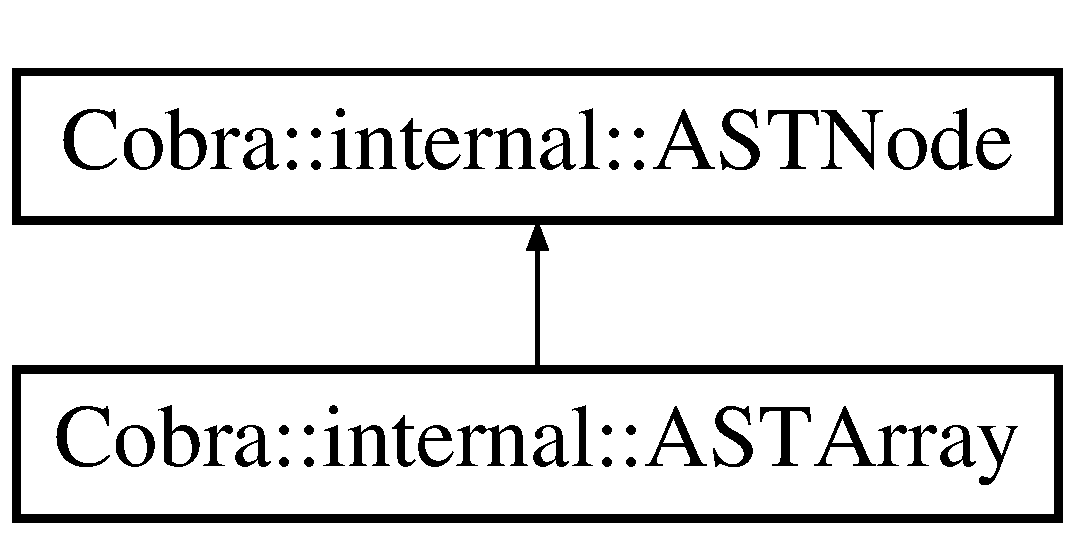
\includegraphics[height=2.000000cm]{class_cobra_1_1internal_1_1_a_s_t_array}
\end{center}
\end{figure}
\subsection*{Public Member Functions}
\begin{DoxyCompactItemize}
\item 
\hypertarget{class_cobra_1_1internal_1_1_a_s_t_array_a7e73df9cce52c269cd22e60bc6483fdf}{{\bfseries A\+S\+T\+Array} (T\+O\+K\+E\+N r\+Type)}\label{class_cobra_1_1internal_1_1_a_s_t_array_a7e73df9cce52c269cd22e60bc6483fdf}

\end{DoxyCompactItemize}
\subsection*{Public Attributes}
\begin{DoxyCompactItemize}
\item 
\hypertarget{class_cobra_1_1internal_1_1_a_s_t_array_a5e06b381684e0af6cd91e7b638172b90}{std\+::vector$<$ \hyperlink{class_cobra_1_1internal_1_1_a_s_t_node}{A\+S\+T\+Node} $\ast$ $>$ {\bfseries value}}\label{class_cobra_1_1internal_1_1_a_s_t_array_a5e06b381684e0af6cd91e7b638172b90}

\item 
\hypertarget{class_cobra_1_1internal_1_1_a_s_t_array_a13ba0e96bfc8ede1589a2da9c4bbcf8b}{T\+O\+K\+E\+N {\bfseries array\+Type}}\label{class_cobra_1_1internal_1_1_a_s_t_array_a13ba0e96bfc8ede1589a2da9c4bbcf8b}

\end{DoxyCompactItemize}


The documentation for this class was generated from the following files\+:\begin{DoxyCompactItemize}
\item 
src/cobra/ast/ast.\+h\item 
src/cobra/ast/ast.\+cc\end{DoxyCompactItemize}

\hypertarget{class_cobra_1_1internal_1_1_a_s_t_array_member_expr}{\section{Cobra\+:\+:internal\+:\+:A\+S\+T\+Array\+Member\+Expr Class Reference}
\label{class_cobra_1_1internal_1_1_a_s_t_array_member_expr}\index{Cobra\+::internal\+::\+A\+S\+T\+Array\+Member\+Expr@{Cobra\+::internal\+::\+A\+S\+T\+Array\+Member\+Expr}}
}
Inheritance diagram for Cobra\+:\+:internal\+:\+:A\+S\+T\+Array\+Member\+Expr\+:\begin{figure}[H]
\begin{center}
\leavevmode
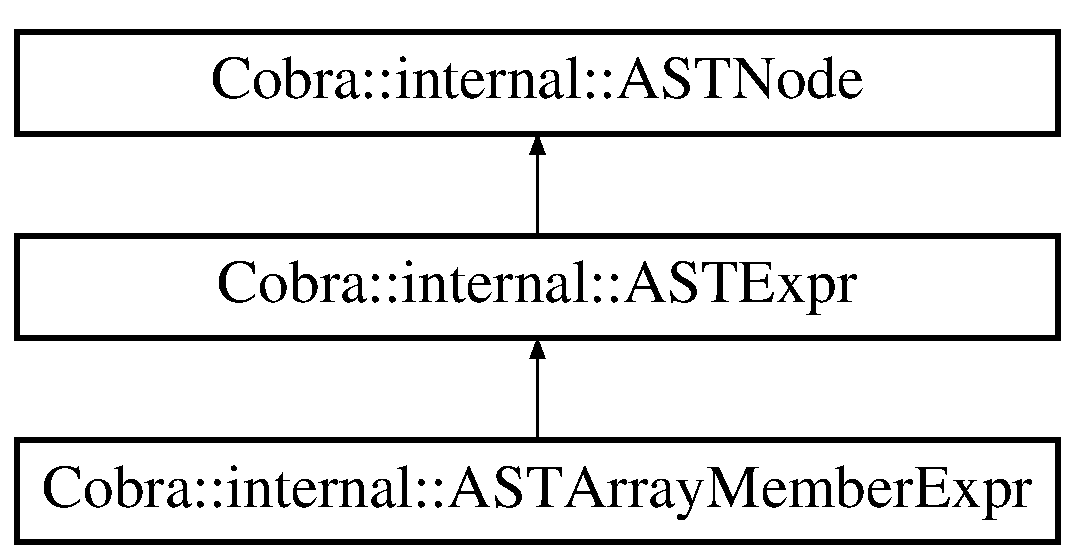
\includegraphics[height=3.000000cm]{class_cobra_1_1internal_1_1_a_s_t_array_member_expr}
\end{center}
\end{figure}
\subsection*{Public Attributes}
\begin{DoxyCompactItemize}
\item 
\hypertarget{class_cobra_1_1internal_1_1_a_s_t_array_member_expr_a922f6f629046bbc5bdf5b6cc7995855a}{\hyperlink{class_cobra_1_1internal_1_1_a_s_t_expr}{A\+S\+T\+Expr} $\ast$ {\bfseries member}}\label{class_cobra_1_1internal_1_1_a_s_t_array_member_expr_a922f6f629046bbc5bdf5b6cc7995855a}

\item 
\hypertarget{class_cobra_1_1internal_1_1_a_s_t_array_member_expr_a082fbdf58b2a807931a81fda004b86f7}{\hyperlink{class_cobra_1_1internal_1_1_a_s_t_expr}{A\+S\+T\+Expr} $\ast$ {\bfseries value}}\label{class_cobra_1_1internal_1_1_a_s_t_array_member_expr_a082fbdf58b2a807931a81fda004b86f7}

\end{DoxyCompactItemize}


The documentation for this class was generated from the following file\+:\begin{DoxyCompactItemize}
\item 
src/cobra/ast/ast.\+h\end{DoxyCompactItemize}

\hypertarget{class_cobra_1_1internal_1_1_a_s_t_binary_expr}{\section{Cobra\+:\+:internal\+:\+:A\+S\+T\+Binary\+Expr Class Reference}
\label{class_cobra_1_1internal_1_1_a_s_t_binary_expr}\index{Cobra\+::internal\+::\+A\+S\+T\+Binary\+Expr@{Cobra\+::internal\+::\+A\+S\+T\+Binary\+Expr}}
}
Inheritance diagram for Cobra\+:\+:internal\+:\+:A\+S\+T\+Binary\+Expr\+:\begin{figure}[H]
\begin{center}
\leavevmode
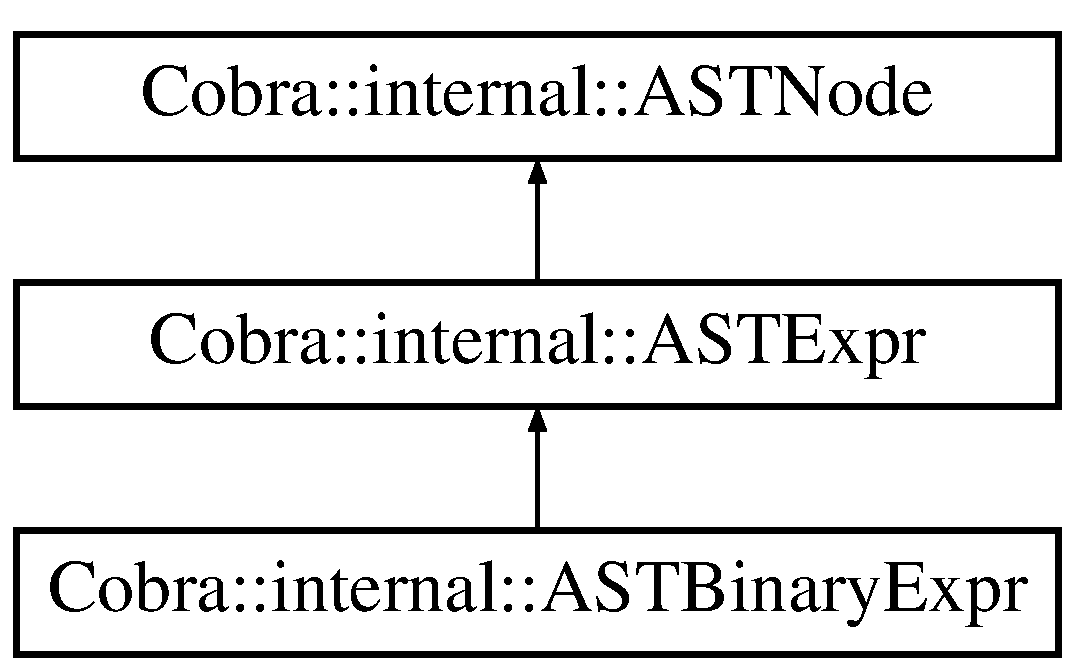
\includegraphics[height=3.000000cm]{class_cobra_1_1internal_1_1_a_s_t_binary_expr}
\end{center}
\end{figure}
\subsection*{Public Attributes}
\begin{DoxyCompactItemize}
\item 
\hypertarget{class_cobra_1_1internal_1_1_a_s_t_binary_expr_aeb1680fce98d2d2b17bf4d8751efea4d}{\hyperlink{class_cobra_1_1internal_1_1_a_s_t_expr}{A\+S\+T\+Expr} $\ast$ {\bfseries Left}}\label{class_cobra_1_1internal_1_1_a_s_t_binary_expr_aeb1680fce98d2d2b17bf4d8751efea4d}

\item 
\hypertarget{class_cobra_1_1internal_1_1_a_s_t_binary_expr_a7b1c52a1e71454681f675401344ea4c9}{\hyperlink{class_cobra_1_1internal_1_1_a_s_t_expr}{A\+S\+T\+Expr} $\ast$ {\bfseries Right}}\label{class_cobra_1_1internal_1_1_a_s_t_binary_expr_a7b1c52a1e71454681f675401344ea4c9}

\item 
\hypertarget{class_cobra_1_1internal_1_1_a_s_t_binary_expr_aa94555a0468455f9ad2d5a7f848d1ef9}{\hyperlink{class_cobra_1_1internal_1_1_token}{Token} $\ast$ {\bfseries op}}\label{class_cobra_1_1internal_1_1_a_s_t_binary_expr_aa94555a0468455f9ad2d5a7f848d1ef9}

\end{DoxyCompactItemize}


The documentation for this class was generated from the following file\+:\begin{DoxyCompactItemize}
\item 
src/cobra/ast/ast.\+h\end{DoxyCompactItemize}

\hypertarget{class_cobra_1_1internal_1_1_a_s_t_block}{\section{Cobra\+:\+:internal\+:\+:A\+S\+T\+Block Class Reference}
\label{class_cobra_1_1internal_1_1_a_s_t_block}\index{Cobra\+::internal\+::\+A\+S\+T\+Block@{Cobra\+::internal\+::\+A\+S\+T\+Block}}
}
Inheritance diagram for Cobra\+:\+:internal\+:\+:A\+S\+T\+Block\+:\begin{figure}[H]
\begin{center}
\leavevmode
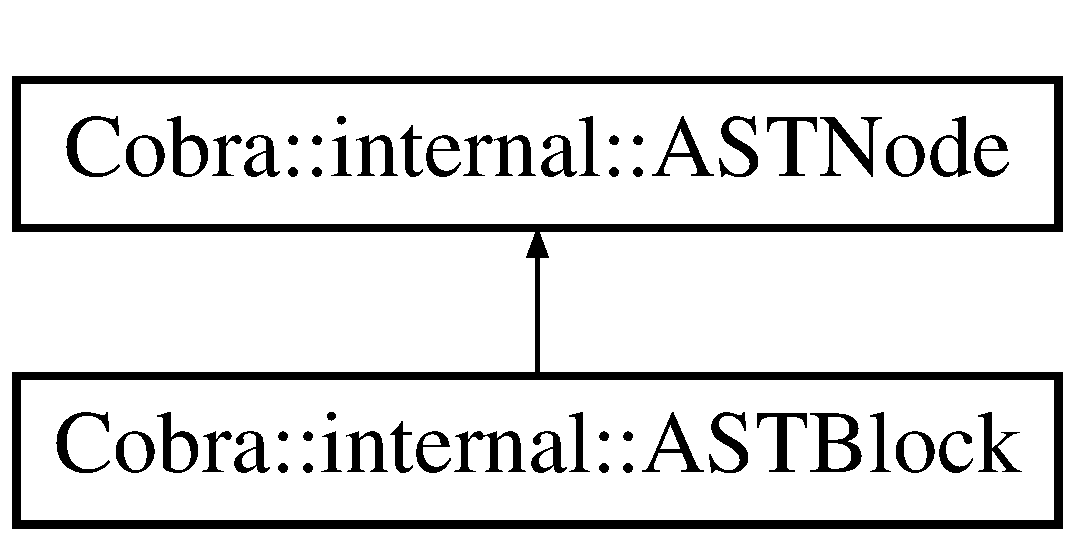
\includegraphics[height=2.000000cm]{class_cobra_1_1internal_1_1_a_s_t_block}
\end{center}
\end{figure}
\subsection*{Public Attributes}
\begin{DoxyCompactItemize}
\item 
\hypertarget{class_cobra_1_1internal_1_1_a_s_t_block_a738bd59c10dea2aef7d0bfed7da854a9}{\hyperlink{class_cobra_1_1internal_1_1_scope}{Scope} $\ast$ {\bfseries scope}}\label{class_cobra_1_1internal_1_1_a_s_t_block_a738bd59c10dea2aef7d0bfed7da854a9}

\end{DoxyCompactItemize}


The documentation for this class was generated from the following files\+:\begin{DoxyCompactItemize}
\item 
src/cobra/ast/ast.\+h\item 
src/cobra/ast/ast.\+cc\end{DoxyCompactItemize}

\hypertarget{class_cobra_1_1internal_1_1_a_s_t_boolean}{\section{Cobra\+:\+:internal\+:\+:A\+S\+T\+Boolean Class Reference}
\label{class_cobra_1_1internal_1_1_a_s_t_boolean}\index{Cobra\+::internal\+::\+A\+S\+T\+Boolean@{Cobra\+::internal\+::\+A\+S\+T\+Boolean}}
}
Inheritance diagram for Cobra\+:\+:internal\+:\+:A\+S\+T\+Boolean\+:\begin{figure}[H]
\begin{center}
\leavevmode
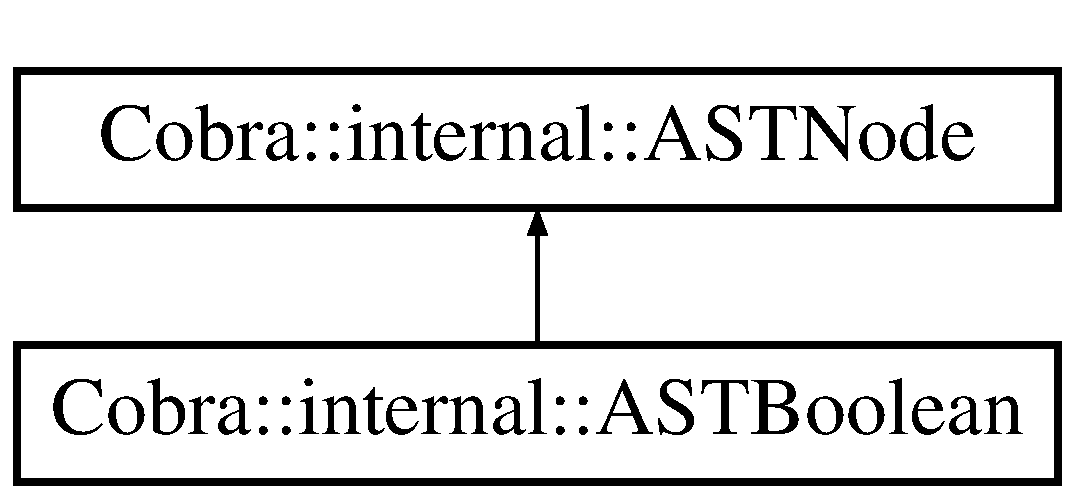
\includegraphics[height=2.000000cm]{class_cobra_1_1internal_1_1_a_s_t_boolean}
\end{center}
\end{figure}
\subsection*{Static Public Member Functions}
\begin{DoxyCompactItemize}
\item 
\hypertarget{class_cobra_1_1internal_1_1_a_s_t_boolean_acaf761398c238a6a614f47e1c13fce83}{static \hyperlink{class_cobra_1_1internal_1_1_a_s_t_boolean}{A\+S\+T\+Boolean} $\ast$ {\bfseries New} (\hyperlink{class_cobra_1_1internal_1_1_isolate}{Isolate} $\ast$iso)}\label{class_cobra_1_1internal_1_1_a_s_t_boolean_acaf761398c238a6a614f47e1c13fce83}

\end{DoxyCompactItemize}
\subsection*{Public Attributes}
\begin{DoxyCompactItemize}
\item 
\hypertarget{class_cobra_1_1internal_1_1_a_s_t_boolean_a029bb02b49553aee23445512eb57afa0}{bool {\bfseries value}}\label{class_cobra_1_1internal_1_1_a_s_t_boolean_a029bb02b49553aee23445512eb57afa0}

\end{DoxyCompactItemize}


The documentation for this class was generated from the following files\+:\begin{DoxyCompactItemize}
\item 
src/cobra/ast/ast.\+h\item 
src/cobra/ast/ast.\+cc\end{DoxyCompactItemize}

\hypertarget{class_cobra_1_1internal_1_1_a_s_t_cast_expr}{\section{Cobra\+:\+:internal\+:\+:A\+S\+T\+Cast\+Expr Class Reference}
\label{class_cobra_1_1internal_1_1_a_s_t_cast_expr}\index{Cobra\+::internal\+::\+A\+S\+T\+Cast\+Expr@{Cobra\+::internal\+::\+A\+S\+T\+Cast\+Expr}}
}
Inheritance diagram for Cobra\+:\+:internal\+:\+:A\+S\+T\+Cast\+Expr\+:\begin{figure}[H]
\begin{center}
\leavevmode
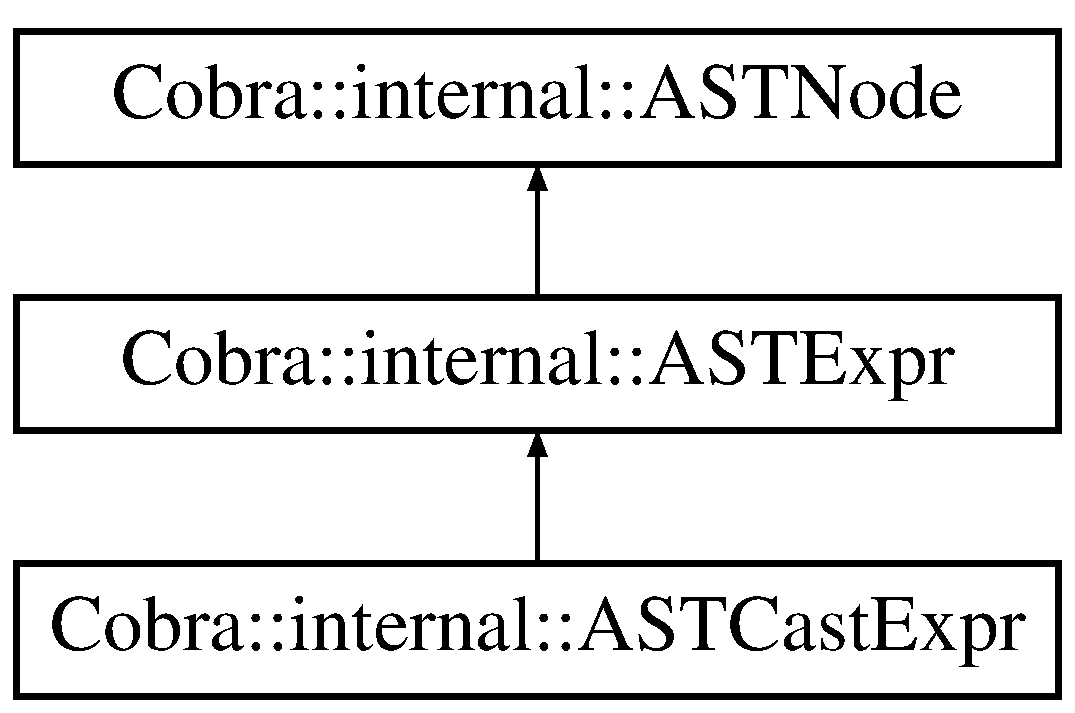
\includegraphics[height=3.000000cm]{class_cobra_1_1internal_1_1_a_s_t_cast_expr}
\end{center}
\end{figure}
\subsection*{Static Public Member Functions}
\begin{DoxyCompactItemize}
\item 
\hypertarget{class_cobra_1_1internal_1_1_a_s_t_cast_expr_ae37ff4d3a4bdd6c16a9bde34b163971d}{static \hyperlink{class_cobra_1_1internal_1_1_a_s_t_cast_expr}{A\+S\+T\+Cast\+Expr} $\ast$ {\bfseries New} (\hyperlink{class_cobra_1_1internal_1_1_isolate}{Isolate} $\ast$iso)}\label{class_cobra_1_1internal_1_1_a_s_t_cast_expr_ae37ff4d3a4bdd6c16a9bde34b163971d}

\end{DoxyCompactItemize}
\subsection*{Public Attributes}
\begin{DoxyCompactItemize}
\item 
\hypertarget{class_cobra_1_1internal_1_1_a_s_t_cast_expr_ae1c831b39b5f0280e17896784dc419fa}{T\+O\+K\+E\+N {\bfseries cast\+Type}}\label{class_cobra_1_1internal_1_1_a_s_t_cast_expr_ae1c831b39b5f0280e17896784dc419fa}

\item 
\hypertarget{class_cobra_1_1internal_1_1_a_s_t_cast_expr_a65dd03166f5fa966c3c9d18fe78a30e3}{\hyperlink{class_cobra_1_1internal_1_1_a_s_t_expr}{A\+S\+T\+Expr} $\ast$ {\bfseries to}}\label{class_cobra_1_1internal_1_1_a_s_t_cast_expr_a65dd03166f5fa966c3c9d18fe78a30e3}

\item 
\hypertarget{class_cobra_1_1internal_1_1_a_s_t_cast_expr_ad3b58a028bdb1241fe1eb98b306fd9cb}{\hyperlink{class_cobra_1_1internal_1_1_a_s_t_expr}{A\+S\+T\+Expr} $\ast$ {\bfseries value}}\label{class_cobra_1_1internal_1_1_a_s_t_cast_expr_ad3b58a028bdb1241fe1eb98b306fd9cb}

\end{DoxyCompactItemize}


The documentation for this class was generated from the following files\+:\begin{DoxyCompactItemize}
\item 
src/cobra/ast/ast.\+h\item 
src/cobra/ast/ast.\+cc\end{DoxyCompactItemize}

\hypertarget{class_cobra_1_1internal_1_1_a_s_t_char}{\section{Cobra\+:\+:internal\+:\+:A\+S\+T\+Char Class Reference}
\label{class_cobra_1_1internal_1_1_a_s_t_char}\index{Cobra\+::internal\+::\+A\+S\+T\+Char@{Cobra\+::internal\+::\+A\+S\+T\+Char}}
}
Inheritance diagram for Cobra\+:\+:internal\+:\+:A\+S\+T\+Char\+:\begin{figure}[H]
\begin{center}
\leavevmode
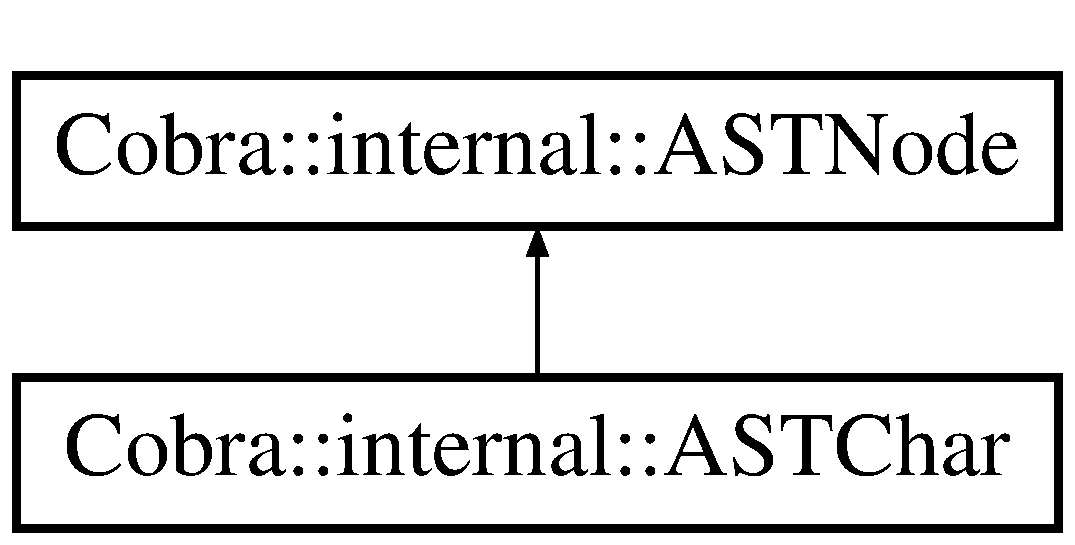
\includegraphics[height=2.000000cm]{class_cobra_1_1internal_1_1_a_s_t_char}
\end{center}
\end{figure}
\subsection*{Static Public Member Functions}
\begin{DoxyCompactItemize}
\item 
\hypertarget{class_cobra_1_1internal_1_1_a_s_t_char_a971799e30af09f339aca8a40d7dad7a7}{static \hyperlink{class_cobra_1_1internal_1_1_a_s_t_char}{A\+S\+T\+Char} $\ast$ {\bfseries New} (\hyperlink{class_cobra_1_1internal_1_1_isolate}{Isolate} $\ast$iso)}\label{class_cobra_1_1internal_1_1_a_s_t_char_a971799e30af09f339aca8a40d7dad7a7}

\end{DoxyCompactItemize}
\subsection*{Public Attributes}
\begin{DoxyCompactItemize}
\item 
\hypertarget{class_cobra_1_1internal_1_1_a_s_t_char_aa8b815df4fb708f5af29f9bb5311967d}{char {\bfseries value}}\label{class_cobra_1_1internal_1_1_a_s_t_char_aa8b815df4fb708f5af29f9bb5311967d}

\end{DoxyCompactItemize}


The documentation for this class was generated from the following files\+:\begin{DoxyCompactItemize}
\item 
src/cobra/ast/ast.\+h\item 
src/cobra/ast/ast.\+cc\end{DoxyCompactItemize}

\hypertarget{class_cobra_1_1internal_1_1_a_s_t_double}{\section{Cobra\+:\+:internal\+:\+:A\+S\+T\+Double Class Reference}
\label{class_cobra_1_1internal_1_1_a_s_t_double}\index{Cobra\+::internal\+::\+A\+S\+T\+Double@{Cobra\+::internal\+::\+A\+S\+T\+Double}}
}
Inheritance diagram for Cobra\+:\+:internal\+:\+:A\+S\+T\+Double\+:\begin{figure}[H]
\begin{center}
\leavevmode
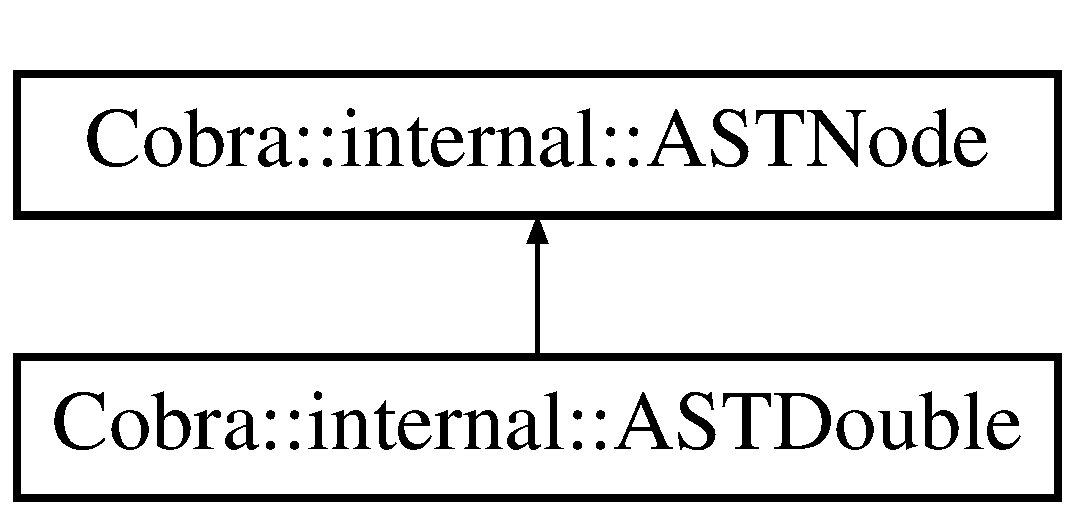
\includegraphics[height=2.000000cm]{class_cobra_1_1internal_1_1_a_s_t_double}
\end{center}
\end{figure}
\subsection*{Static Public Member Functions}
\begin{DoxyCompactItemize}
\item 
\hypertarget{class_cobra_1_1internal_1_1_a_s_t_double_a6c84e6897b4f7a67e074a88c355034c1}{static \hyperlink{class_cobra_1_1internal_1_1_a_s_t_double}{A\+S\+T\+Double} $\ast$ {\bfseries New} (\hyperlink{class_cobra_1_1internal_1_1_isolate}{Isolate} $\ast$iso)}\label{class_cobra_1_1internal_1_1_a_s_t_double_a6c84e6897b4f7a67e074a88c355034c1}

\end{DoxyCompactItemize}
\subsection*{Public Attributes}
\begin{DoxyCompactItemize}
\item 
\hypertarget{class_cobra_1_1internal_1_1_a_s_t_double_adb8d73d965bffb93e8caab014e3f1241}{double {\bfseries value}}\label{class_cobra_1_1internal_1_1_a_s_t_double_adb8d73d965bffb93e8caab014e3f1241}

\end{DoxyCompactItemize}


The documentation for this class was generated from the following files\+:\begin{DoxyCompactItemize}
\item 
src/cobra/ast/ast.\+h\item 
src/cobra/ast/ast.\+cc\end{DoxyCompactItemize}

\hypertarget{class_cobra_1_1internal_1_1_a_s_t_else}{\section{Cobra\+:\+:internal\+:\+:A\+S\+T\+Else Class Reference}
\label{class_cobra_1_1internal_1_1_a_s_t_else}\index{Cobra\+::internal\+::\+A\+S\+T\+Else@{Cobra\+::internal\+::\+A\+S\+T\+Else}}
}
Inheritance diagram for Cobra\+:\+:internal\+:\+:A\+S\+T\+Else\+:\begin{figure}[H]
\begin{center}
\leavevmode
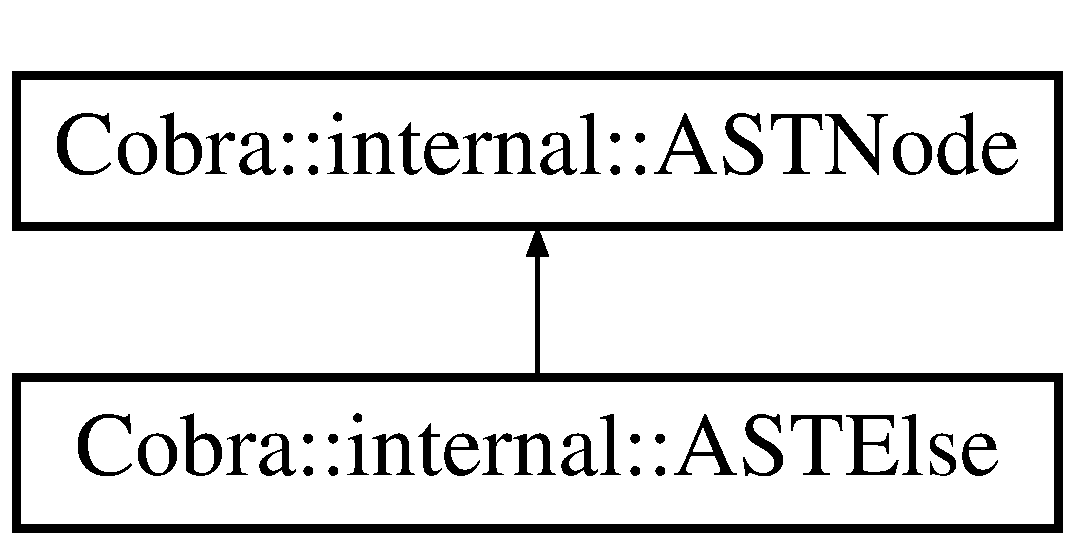
\includegraphics[height=2.000000cm]{class_cobra_1_1internal_1_1_a_s_t_else}
\end{center}
\end{figure}
\subsection*{Static Public Member Functions}
\begin{DoxyCompactItemize}
\item 
\hypertarget{class_cobra_1_1internal_1_1_a_s_t_else_ad40b80353d4b708ef4378e489cf7b6d7}{static \hyperlink{class_cobra_1_1internal_1_1_a_s_t_else}{A\+S\+T\+Else} $\ast$ {\bfseries New} (\hyperlink{class_cobra_1_1internal_1_1_isolate}{Isolate} $\ast$iso)}\label{class_cobra_1_1internal_1_1_a_s_t_else_ad40b80353d4b708ef4378e489cf7b6d7}

\end{DoxyCompactItemize}
\subsection*{Public Attributes}
\begin{DoxyCompactItemize}
\item 
\hypertarget{class_cobra_1_1internal_1_1_a_s_t_else_a6dbc7cd7172739f57de42510cfc261ca}{\hyperlink{class_cobra_1_1internal_1_1_a_s_t_expr}{A\+S\+T\+Expr} $\ast$ {\bfseries conditions}}\label{class_cobra_1_1internal_1_1_a_s_t_else_a6dbc7cd7172739f57de42510cfc261ca}

\item 
\hypertarget{class_cobra_1_1internal_1_1_a_s_t_else_a7353693c92ca38e5bef78ee483db681a}{\hyperlink{class_cobra_1_1internal_1_1_a_s_t_block}{A\+S\+T\+Block} $\ast$ {\bfseries block}}\label{class_cobra_1_1internal_1_1_a_s_t_else_a7353693c92ca38e5bef78ee483db681a}

\item 
\hypertarget{class_cobra_1_1internal_1_1_a_s_t_else_a61d07a78a5462b42d89428825cd7f168}{\hyperlink{class_cobra_1_1internal_1_1_a_s_t_if}{A\+S\+T\+If} $\ast$ {\bfseries if\+Stmt}}\label{class_cobra_1_1internal_1_1_a_s_t_else_a61d07a78a5462b42d89428825cd7f168}

\end{DoxyCompactItemize}


The documentation for this class was generated from the following files\+:\begin{DoxyCompactItemize}
\item 
src/cobra/ast/ast.\+h\item 
src/cobra/ast/ast.\+cc\end{DoxyCompactItemize}

\hypertarget{class_cobra_1_1internal_1_1_a_s_t_expr}{\section{Cobra\+:\+:internal\+:\+:A\+S\+T\+Expr Class Reference}
\label{class_cobra_1_1internal_1_1_a_s_t_expr}\index{Cobra\+::internal\+::\+A\+S\+T\+Expr@{Cobra\+::internal\+::\+A\+S\+T\+Expr}}
}
Inheritance diagram for Cobra\+:\+:internal\+:\+:A\+S\+T\+Expr\+:\begin{figure}[H]
\begin{center}
\leavevmode
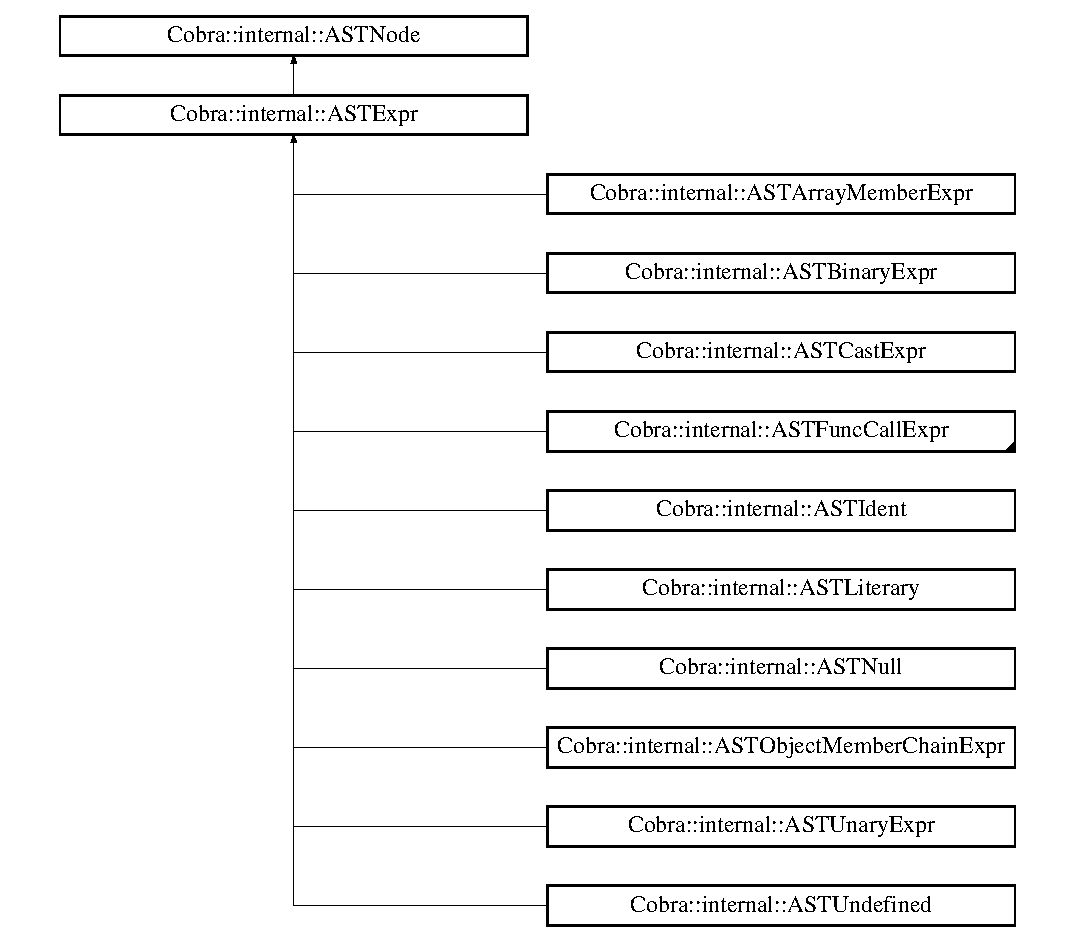
\includegraphics[height=0.872727cm]{class_cobra_1_1internal_1_1_a_s_t_expr}
\end{center}
\end{figure}
\subsection*{Public Attributes}
\begin{DoxyCompactItemize}
\item 
\hypertarget{class_cobra_1_1internal_1_1_a_s_t_expr_af1bf2806f323bc63de0a3aab9f181923}{\hyperlink{class_cobra_1_1internal_1_1_a_s_t_expr}{A\+S\+T\+Expr} $\ast$ {\bfseries value}}\label{class_cobra_1_1internal_1_1_a_s_t_expr_af1bf2806f323bc63de0a3aab9f181923}

\item 
\hypertarget{class_cobra_1_1internal_1_1_a_s_t_expr_a88bfbf832e3b00a89ba949562f573919}{T\+O\+K\+E\+N {\bfseries assign\+Type}}\label{class_cobra_1_1internal_1_1_a_s_t_expr_a88bfbf832e3b00a89ba949562f573919}

\end{DoxyCompactItemize}


The documentation for this class was generated from the following files\+:\begin{DoxyCompactItemize}
\item 
src/cobra/ast/ast.\+h\item 
src/cobra/ast/ast.\+cc\end{DoxyCompactItemize}

\hypertarget{class_cobra_1_1internal_1_1_a_s_t_file}{\section{Cobra\+:\+:internal\+:\+:A\+S\+T\+File Class Reference}
\label{class_cobra_1_1internal_1_1_a_s_t_file}\index{Cobra\+::internal\+::\+A\+S\+T\+File@{Cobra\+::internal\+::\+A\+S\+T\+File}}
}
Inheritance diagram for Cobra\+:\+:internal\+:\+:A\+S\+T\+File\+:\begin{figure}[H]
\begin{center}
\leavevmode
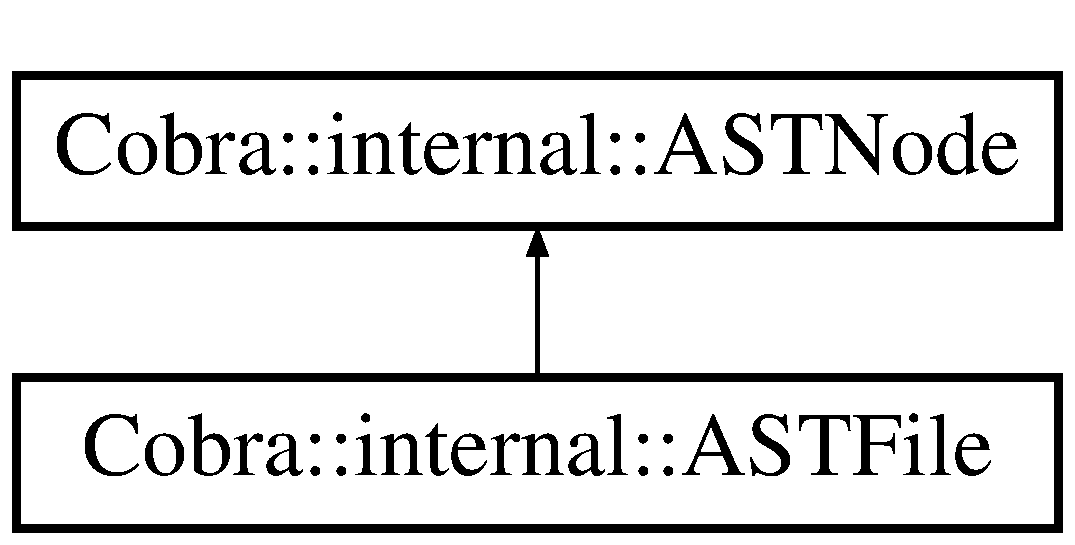
\includegraphics[height=2.000000cm]{class_cobra_1_1internal_1_1_a_s_t_file}
\end{center}
\end{figure}
\subsection*{Public Attributes}
\begin{DoxyCompactItemize}
\item 
\hypertarget{class_cobra_1_1internal_1_1_a_s_t_file_affc71f3bf233586e51d4c5b0aa938962}{\hyperlink{class_cobra_1_1internal_1_1_scope}{Scope} $\ast$ {\bfseries scope}}\label{class_cobra_1_1internal_1_1_a_s_t_file_affc71f3bf233586e51d4c5b0aa938962}

\end{DoxyCompactItemize}


The documentation for this class was generated from the following files\+:\begin{DoxyCompactItemize}
\item 
src/cobra/ast/ast.\+h\item 
src/cobra/ast/ast.\+cc\end{DoxyCompactItemize}

\hypertarget{class_cobra_1_1internal_1_1_a_s_t_float}{\section{Cobra\+:\+:internal\+:\+:A\+S\+T\+Float Class Reference}
\label{class_cobra_1_1internal_1_1_a_s_t_float}\index{Cobra\+::internal\+::\+A\+S\+T\+Float@{Cobra\+::internal\+::\+A\+S\+T\+Float}}
}
Inheritance diagram for Cobra\+:\+:internal\+:\+:A\+S\+T\+Float\+:\begin{figure}[H]
\begin{center}
\leavevmode
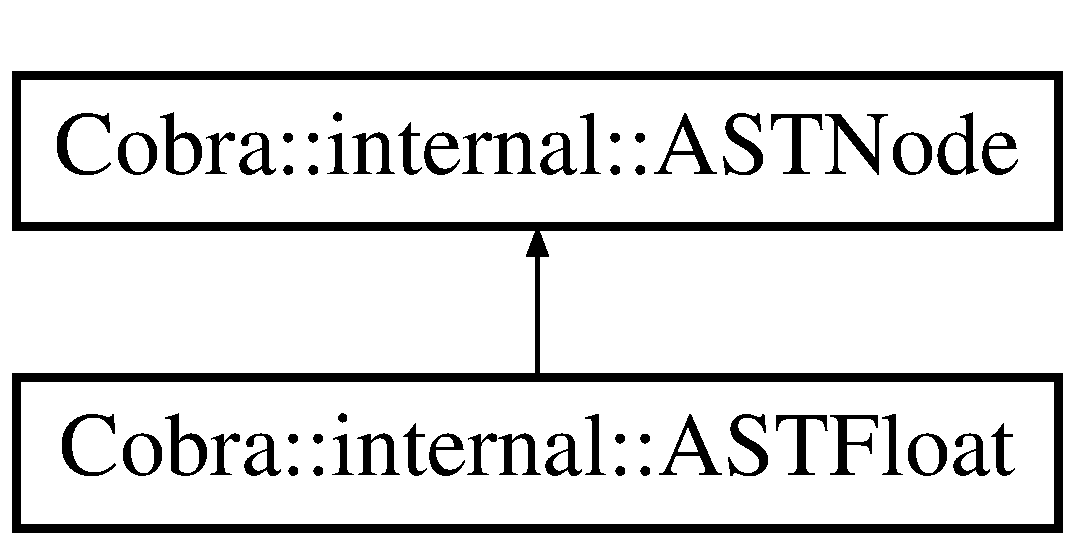
\includegraphics[height=2.000000cm]{class_cobra_1_1internal_1_1_a_s_t_float}
\end{center}
\end{figure}
\subsection*{Static Public Member Functions}
\begin{DoxyCompactItemize}
\item 
\hypertarget{class_cobra_1_1internal_1_1_a_s_t_float_a36a9b861c31edc9e55aad0eaf4e4ec9c}{static \hyperlink{class_cobra_1_1internal_1_1_a_s_t_float}{A\+S\+T\+Float} $\ast$ {\bfseries New} (\hyperlink{class_cobra_1_1internal_1_1_isolate}{Isolate} $\ast$iso)}\label{class_cobra_1_1internal_1_1_a_s_t_float_a36a9b861c31edc9e55aad0eaf4e4ec9c}

\end{DoxyCompactItemize}
\subsection*{Public Attributes}
\begin{DoxyCompactItemize}
\item 
\hypertarget{class_cobra_1_1internal_1_1_a_s_t_float_ae6955ebe85532ecd20cc8dd4f721f6fe}{float {\bfseries value}}\label{class_cobra_1_1internal_1_1_a_s_t_float_ae6955ebe85532ecd20cc8dd4f721f6fe}

\end{DoxyCompactItemize}


The documentation for this class was generated from the following files\+:\begin{DoxyCompactItemize}
\item 
src/cobra/ast/ast.\+h\item 
src/cobra/ast/ast.\+cc\end{DoxyCompactItemize}

\hypertarget{class_cobra_1_1internal_1_1_a_s_t_for}{\section{Cobra\+:\+:internal\+:\+:A\+S\+T\+For Class Reference}
\label{class_cobra_1_1internal_1_1_a_s_t_for}\index{Cobra\+::internal\+::\+A\+S\+T\+For@{Cobra\+::internal\+::\+A\+S\+T\+For}}
}
Inheritance diagram for Cobra\+:\+:internal\+:\+:A\+S\+T\+For\+:\begin{figure}[H]
\begin{center}
\leavevmode
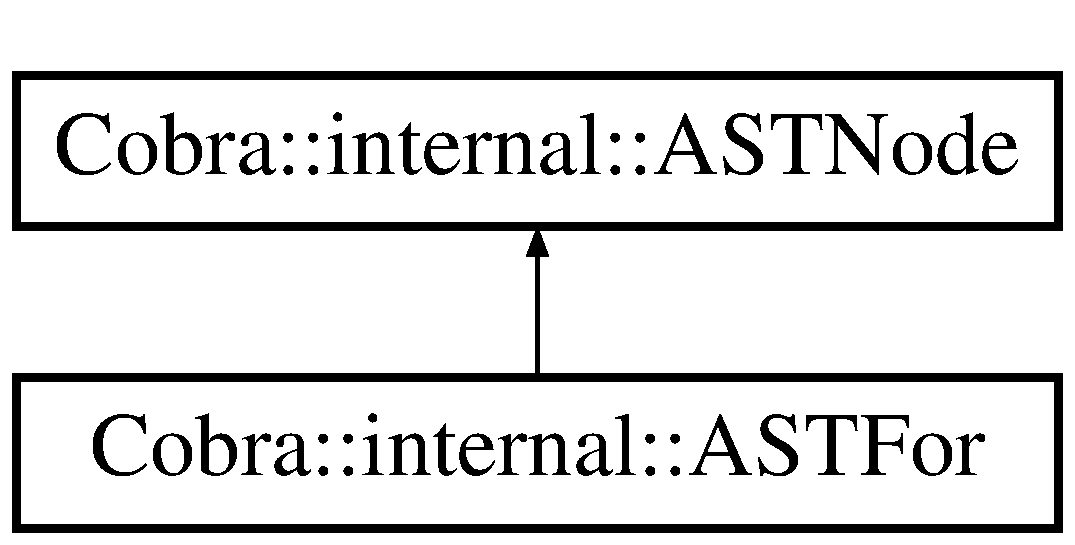
\includegraphics[height=2.000000cm]{class_cobra_1_1internal_1_1_a_s_t_for}
\end{center}
\end{figure}
\subsection*{Public Attributes}
\begin{DoxyCompactItemize}
\item 
\hypertarget{class_cobra_1_1internal_1_1_a_s_t_for_a61962164f3d93fc5d680090b056ff8b7}{\hyperlink{class_cobra_1_1internal_1_1_a_s_t_node}{A\+S\+T\+Node} $\ast$ {\bfseries var}}\label{class_cobra_1_1internal_1_1_a_s_t_for_a61962164f3d93fc5d680090b056ff8b7}

\item 
\hypertarget{class_cobra_1_1internal_1_1_a_s_t_for_ae895f2e05ca9372a84c5ddeb75742386}{\hyperlink{class_cobra_1_1internal_1_1_a_s_t_expr}{A\+S\+T\+Expr} $\ast$ {\bfseries conditions}}\label{class_cobra_1_1internal_1_1_a_s_t_for_ae895f2e05ca9372a84c5ddeb75742386}

\item 
\hypertarget{class_cobra_1_1internal_1_1_a_s_t_for_aabc648bff8efded5efdfeb4e386b40fa}{\hyperlink{class_cobra_1_1internal_1_1_a_s_t_expr}{A\+S\+T\+Expr} $\ast$ {\bfseries iterator}}\label{class_cobra_1_1internal_1_1_a_s_t_for_aabc648bff8efded5efdfeb4e386b40fa}

\item 
\hypertarget{class_cobra_1_1internal_1_1_a_s_t_for_a2e7a7694dc5527a8936305e70e7438ed}{\hyperlink{class_cobra_1_1internal_1_1_a_s_t_block}{A\+S\+T\+Block} $\ast$ {\bfseries block}}\label{class_cobra_1_1internal_1_1_a_s_t_for_a2e7a7694dc5527a8936305e70e7438ed}

\end{DoxyCompactItemize}


The documentation for this class was generated from the following files\+:\begin{DoxyCompactItemize}
\item 
src/cobra/ast/ast.\+h\item 
src/cobra/ast/ast.\+cc\end{DoxyCompactItemize}

\hypertarget{class_cobra_1_1internal_1_1_a_s_t_func}{\section{Cobra\+:\+:internal\+:\+:A\+S\+T\+Func Class Reference}
\label{class_cobra_1_1internal_1_1_a_s_t_func}\index{Cobra\+::internal\+::\+A\+S\+T\+Func@{Cobra\+::internal\+::\+A\+S\+T\+Func}}
}
Inheritance diagram for Cobra\+:\+:internal\+:\+:A\+S\+T\+Func\+:\begin{figure}[H]
\begin{center}
\leavevmode
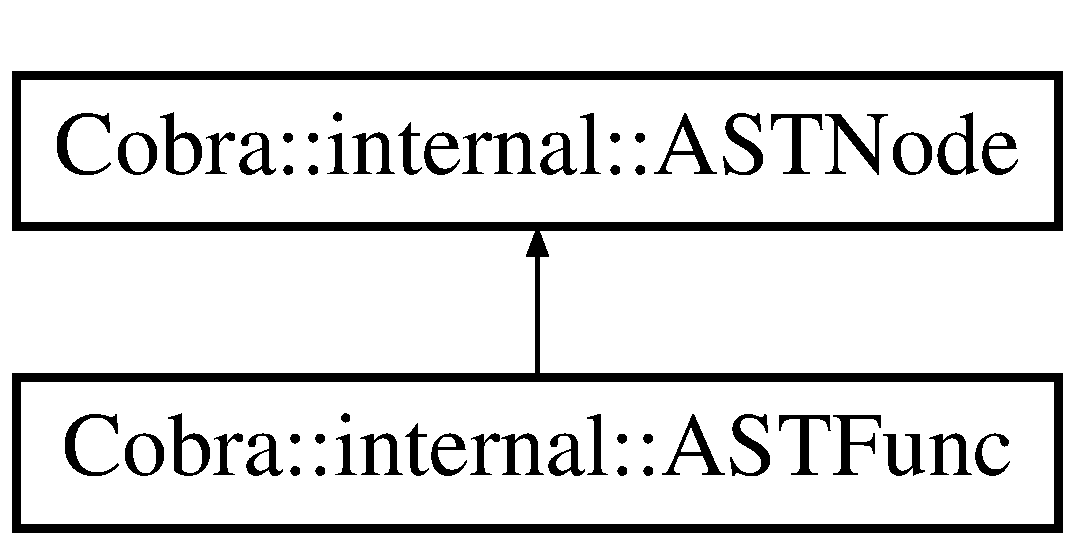
\includegraphics[height=2.000000cm]{class_cobra_1_1internal_1_1_a_s_t_func}
\end{center}
\end{figure}
\subsection*{Public Attributes}
\begin{DoxyCompactItemize}
\item 
\hypertarget{class_cobra_1_1internal_1_1_a_s_t_func_a6e67ed4f5bba2a0cf2a65cdc72180730}{\hyperlink{class_cobra_1_1internal_1_1_a_s_t_block}{A\+S\+T\+Block} $\ast$ {\bfseries body}}\label{class_cobra_1_1internal_1_1_a_s_t_func_a6e67ed4f5bba2a0cf2a65cdc72180730}

\item 
\hypertarget{class_cobra_1_1internal_1_1_a_s_t_func_a21e9a01b1a5d2596bbd7292bf384d18a}{std\+::map$<$ std\+::string, \hyperlink{class_cobra_1_1internal_1_1_a_s_t_node}{A\+S\+T\+Node} $\ast$ $>$ {\bfseries args}}\label{class_cobra_1_1internal_1_1_a_s_t_func_a21e9a01b1a5d2596bbd7292bf384d18a}

\item 
\hypertarget{class_cobra_1_1internal_1_1_a_s_t_func_a71cd104c6887f10e539264b9a529dd4e}{std\+::vector$<$ \hyperlink{class_cobra_1_1internal_1_1_a_s_t_node}{A\+S\+T\+Node} $\ast$ $>$ {\bfseries ordered}}\label{class_cobra_1_1internal_1_1_a_s_t_func_a71cd104c6887f10e539264b9a529dd4e}

\end{DoxyCompactItemize}


The documentation for this class was generated from the following files\+:\begin{DoxyCompactItemize}
\item 
src/cobra/ast/ast.\+h\item 
src/cobra/ast/ast.\+cc\end{DoxyCompactItemize}

\hypertarget{class_cobra_1_1internal_1_1_a_s_t_func_call_expr}{\section{Cobra\+:\+:internal\+:\+:A\+S\+T\+Func\+Call\+Expr Class Reference}
\label{class_cobra_1_1internal_1_1_a_s_t_func_call_expr}\index{Cobra\+::internal\+::\+A\+S\+T\+Func\+Call\+Expr@{Cobra\+::internal\+::\+A\+S\+T\+Func\+Call\+Expr}}
}
Inheritance diagram for Cobra\+:\+:internal\+:\+:A\+S\+T\+Func\+Call\+Expr\+:\begin{figure}[H]
\begin{center}
\leavevmode
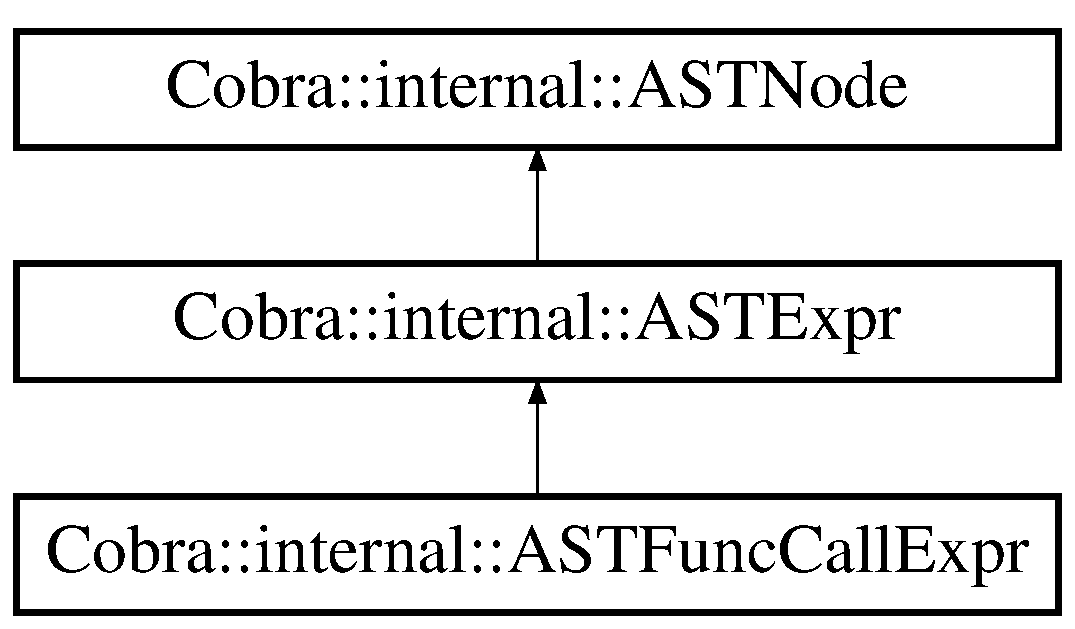
\includegraphics[height=3.000000cm]{class_cobra_1_1internal_1_1_a_s_t_func_call_expr}
\end{center}
\end{figure}
\subsection*{Public Attributes}
\begin{DoxyCompactItemize}
\item 
\hypertarget{class_cobra_1_1internal_1_1_a_s_t_func_call_expr_aa753794f6a51fe645d6168aa4f83c594}{std\+::vector$<$ \hyperlink{class_cobra_1_1internal_1_1_a_s_t_expr}{A\+S\+T\+Expr} $\ast$ $>$ {\bfseries params}}\label{class_cobra_1_1internal_1_1_a_s_t_func_call_expr_aa753794f6a51fe645d6168aa4f83c594}

\item 
\hypertarget{class_cobra_1_1internal_1_1_a_s_t_func_call_expr_ac2d3cd56d13cd40bae1eb030183e2d1f}{int {\bfseries pos}}\label{class_cobra_1_1internal_1_1_a_s_t_func_call_expr_ac2d3cd56d13cd40bae1eb030183e2d1f}

\item 
\hypertarget{class_cobra_1_1internal_1_1_a_s_t_func_call_expr_a5842d495d42a61e1504dec7ca8a8e4a5}{bool {\bfseries is\+New}}\label{class_cobra_1_1internal_1_1_a_s_t_func_call_expr_a5842d495d42a61e1504dec7ca8a8e4a5}

\item 
\hypertarget{class_cobra_1_1internal_1_1_a_s_t_func_call_expr_a2cbcc879dc96092f1a8a627d85524b69}{\hyperlink{class_cobra_1_1internal_1_1_a_s_t_func}{A\+S\+T\+Func} $\ast$ {\bfseries func}}\label{class_cobra_1_1internal_1_1_a_s_t_func_call_expr_a2cbcc879dc96092f1a8a627d85524b69}

\item 
\hypertarget{class_cobra_1_1internal_1_1_a_s_t_func_call_expr_a28afbf7c743500c44ca999c95f1f2346}{\hyperlink{class_cobra_1_1internal_1_1_scope}{Scope} $\ast$ {\bfseries scope}}\label{class_cobra_1_1internal_1_1_a_s_t_func_call_expr_a28afbf7c743500c44ca999c95f1f2346}

\end{DoxyCompactItemize}


The documentation for this class was generated from the following file\+:\begin{DoxyCompactItemize}
\item 
src/cobra/ast/ast.\+h\end{DoxyCompactItemize}

\hypertarget{class_cobra_1_1internal_1_1_a_s_t_ident}{\section{Cobra\+:\+:internal\+:\+:A\+S\+T\+Ident Class Reference}
\label{class_cobra_1_1internal_1_1_a_s_t_ident}\index{Cobra\+::internal\+::\+A\+S\+T\+Ident@{Cobra\+::internal\+::\+A\+S\+T\+Ident}}
}
Inheritance diagram for Cobra\+:\+:internal\+:\+:A\+S\+T\+Ident\+:\begin{figure}[H]
\begin{center}
\leavevmode
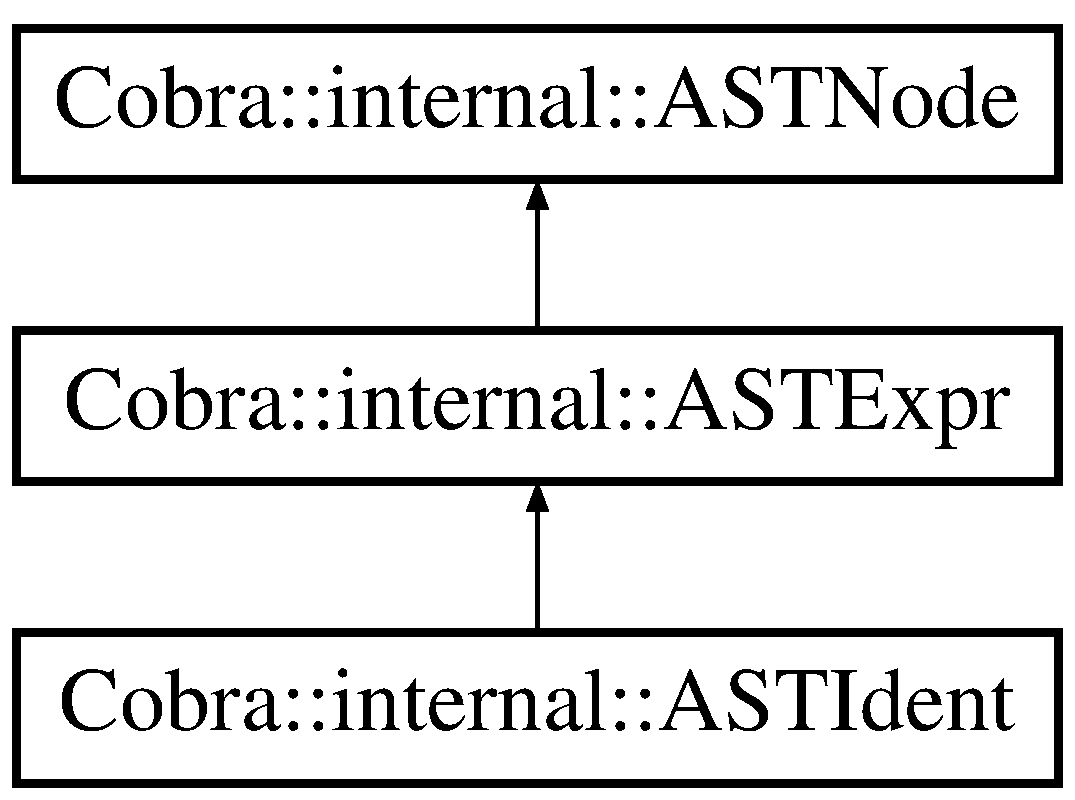
\includegraphics[height=3.000000cm]{class_cobra_1_1internal_1_1_a_s_t_ident}
\end{center}
\end{figure}
\subsection*{Public Attributes}
\begin{DoxyCompactItemize}
\item 
\hypertarget{class_cobra_1_1internal_1_1_a_s_t_ident_ab097c56a4c95a65cb9d1396fcbfcbca8}{int {\bfseries pos}}\label{class_cobra_1_1internal_1_1_a_s_t_ident_ab097c56a4c95a65cb9d1396fcbfcbca8}

\item 
\hypertarget{class_cobra_1_1internal_1_1_a_s_t_ident_a2cab07f99a65917af3a354f99fbbd763}{bool {\bfseries inc}}\label{class_cobra_1_1internal_1_1_a_s_t_ident_a2cab07f99a65917af3a354f99fbbd763}

\item 
\hypertarget{class_cobra_1_1internal_1_1_a_s_t_ident_a51b08c5ac2daa8c97ad2ccf978b946a4}{bool {\bfseries dec}}\label{class_cobra_1_1internal_1_1_a_s_t_ident_a51b08c5ac2daa8c97ad2ccf978b946a4}

\item 
\hypertarget{class_cobra_1_1internal_1_1_a_s_t_ident_aa159b779de1eeb047d3ba7a0977d4e5f}{bool {\bfseries pre}}\label{class_cobra_1_1internal_1_1_a_s_t_ident_aa159b779de1eeb047d3ba7a0977d4e5f}

\item 
\hypertarget{class_cobra_1_1internal_1_1_a_s_t_ident_a0183fff508335a94f78c6ea6050b1574}{bool {\bfseries post}}\label{class_cobra_1_1internal_1_1_a_s_t_ident_a0183fff508335a94f78c6ea6050b1574}

\item 
\hypertarget{class_cobra_1_1internal_1_1_a_s_t_ident_a95f693066082ffed605899d41f37c3a5}{\hyperlink{class_cobra_1_1internal_1_1_a_s_t_node}{A\+S\+T\+Node} $\ast$ {\bfseries value}}\label{class_cobra_1_1internal_1_1_a_s_t_ident_a95f693066082ffed605899d41f37c3a5}

\end{DoxyCompactItemize}


The documentation for this class was generated from the following file\+:\begin{DoxyCompactItemize}
\item 
src/cobra/ast/ast.\+h\end{DoxyCompactItemize}

\hypertarget{class_cobra_1_1internal_1_1_a_s_t_if}{\section{Cobra\+:\+:internal\+:\+:A\+S\+T\+If Class Reference}
\label{class_cobra_1_1internal_1_1_a_s_t_if}\index{Cobra\+::internal\+::\+A\+S\+T\+If@{Cobra\+::internal\+::\+A\+S\+T\+If}}
}
Inheritance diagram for Cobra\+:\+:internal\+:\+:A\+S\+T\+If\+:\begin{figure}[H]
\begin{center}
\leavevmode
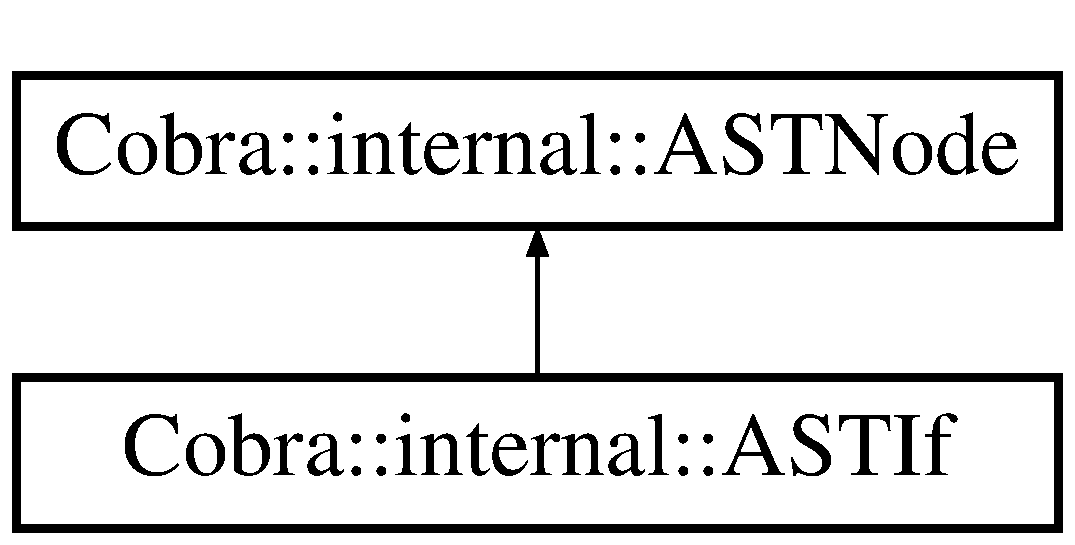
\includegraphics[height=2.000000cm]{class_cobra_1_1internal_1_1_a_s_t_if}
\end{center}
\end{figure}
\subsection*{Static Public Member Functions}
\begin{DoxyCompactItemize}
\item 
\hypertarget{class_cobra_1_1internal_1_1_a_s_t_if_a43fd97fdb0a7c5854dcc82553dd2e1f6}{static \hyperlink{class_cobra_1_1internal_1_1_a_s_t_if}{A\+S\+T\+If} $\ast$ {\bfseries New} (\hyperlink{class_cobra_1_1internal_1_1_isolate}{Isolate} $\ast$iso)}\label{class_cobra_1_1internal_1_1_a_s_t_if_a43fd97fdb0a7c5854dcc82553dd2e1f6}

\end{DoxyCompactItemize}
\subsection*{Public Attributes}
\begin{DoxyCompactItemize}
\item 
\hypertarget{class_cobra_1_1internal_1_1_a_s_t_if_a8131dd336fcda4d14ee7f6ed6e1a4807}{\hyperlink{class_cobra_1_1internal_1_1_a_s_t_expr}{A\+S\+T\+Expr} $\ast$ {\bfseries conditions}}\label{class_cobra_1_1internal_1_1_a_s_t_if_a8131dd336fcda4d14ee7f6ed6e1a4807}

\item 
\hypertarget{class_cobra_1_1internal_1_1_a_s_t_if_a487d09082eab4efc05cb3415987fc0b9}{\hyperlink{class_cobra_1_1internal_1_1_a_s_t_block}{A\+S\+T\+Block} $\ast$ {\bfseries block}}\label{class_cobra_1_1internal_1_1_a_s_t_if_a487d09082eab4efc05cb3415987fc0b9}

\end{DoxyCompactItemize}


The documentation for this class was generated from the following files\+:\begin{DoxyCompactItemize}
\item 
src/cobra/ast/ast.\+h\item 
src/cobra/ast/ast.\+cc\end{DoxyCompactItemize}

\hypertarget{class_cobra_1_1internal_1_1_a_s_t_import}{\section{Cobra\+:\+:internal\+:\+:A\+S\+T\+Import Class Reference}
\label{class_cobra_1_1internal_1_1_a_s_t_import}\index{Cobra\+::internal\+::\+A\+S\+T\+Import@{Cobra\+::internal\+::\+A\+S\+T\+Import}}
}
Inheritance diagram for Cobra\+:\+:internal\+:\+:A\+S\+T\+Import\+:\begin{figure}[H]
\begin{center}
\leavevmode
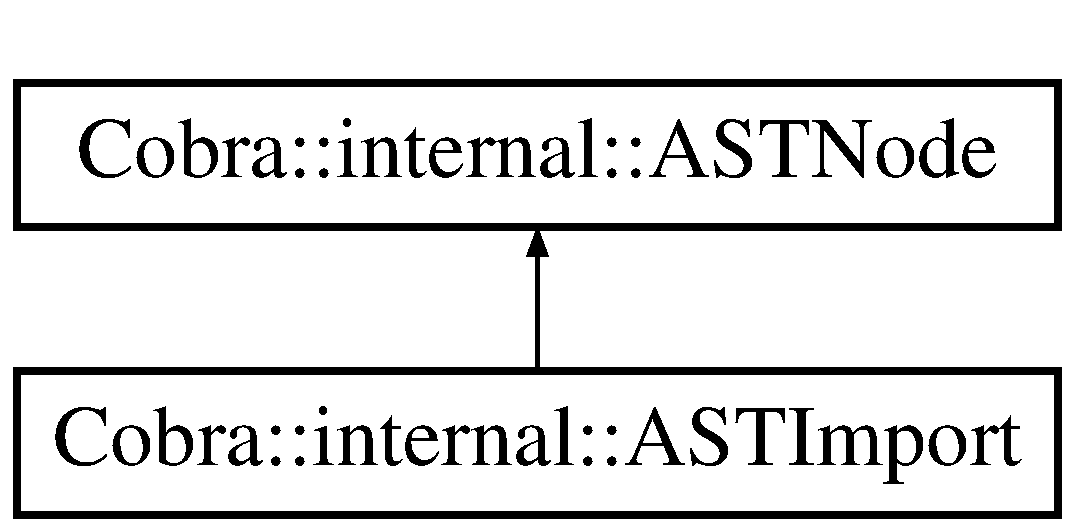
\includegraphics[height=2.000000cm]{class_cobra_1_1internal_1_1_a_s_t_import}
\end{center}
\end{figure}
\subsection*{Public Attributes}
\begin{DoxyCompactItemize}
\item 
\hypertarget{class_cobra_1_1internal_1_1_a_s_t_import_a69e0166ecf3c002a600cbeb1aaa71203}{std\+::string {\bfseries name}}\label{class_cobra_1_1internal_1_1_a_s_t_import_a69e0166ecf3c002a600cbeb1aaa71203}

\item 
\hypertarget{class_cobra_1_1internal_1_1_a_s_t_import_a813737b31c56fe6aed198af56605c2ce}{std\+::string {\bfseries alias}}\label{class_cobra_1_1internal_1_1_a_s_t_import_a813737b31c56fe6aed198af56605c2ce}

\end{DoxyCompactItemize}


The documentation for this class was generated from the following file\+:\begin{DoxyCompactItemize}
\item 
src/cobra/ast/ast.\+h\end{DoxyCompactItemize}

\hypertarget{class_cobra_1_1internal_1_1_a_s_t_include}{\section{Cobra\+:\+:internal\+:\+:A\+S\+T\+Include Class Reference}
\label{class_cobra_1_1internal_1_1_a_s_t_include}\index{Cobra\+::internal\+::\+A\+S\+T\+Include@{Cobra\+::internal\+::\+A\+S\+T\+Include}}
}
Inheritance diagram for Cobra\+:\+:internal\+:\+:A\+S\+T\+Include\+:\begin{figure}[H]
\begin{center}
\leavevmode
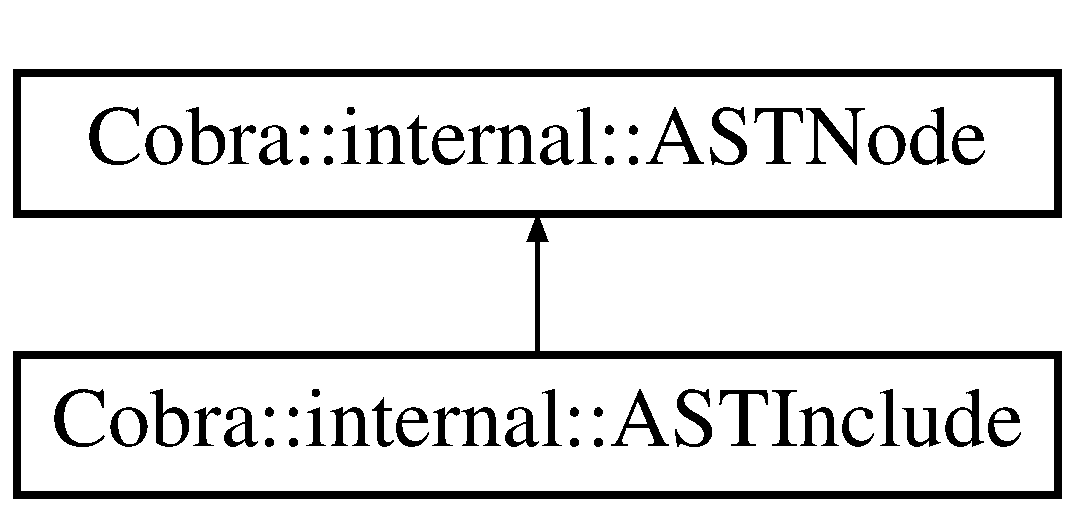
\includegraphics[height=2.000000cm]{class_cobra_1_1internal_1_1_a_s_t_include}
\end{center}
\end{figure}
\subsection*{Public Attributes}
\begin{DoxyCompactItemize}
\item 
\hypertarget{class_cobra_1_1internal_1_1_a_s_t_include_adebc903664510cde12c21e263a3b5df7}{std\+::string {\bfseries name}}\label{class_cobra_1_1internal_1_1_a_s_t_include_adebc903664510cde12c21e263a3b5df7}

\item 
\hypertarget{class_cobra_1_1internal_1_1_a_s_t_include_a194048f23414ee955145161fad552e21}{std\+::string {\bfseries alias}}\label{class_cobra_1_1internal_1_1_a_s_t_include_a194048f23414ee955145161fad552e21}

\item 
\hypertarget{class_cobra_1_1internal_1_1_a_s_t_include_a7af285224c23c6b86295d5434c6a9cc3}{\hyperlink{class_cobra_1_1internal_1_1_a_s_t_file}{A\+S\+T\+File} $\ast$ {\bfseries file}}\label{class_cobra_1_1internal_1_1_a_s_t_include_a7af285224c23c6b86295d5434c6a9cc3}

\end{DoxyCompactItemize}


The documentation for this class was generated from the following file\+:\begin{DoxyCompactItemize}
\item 
src/cobra/ast/ast.\+h\end{DoxyCompactItemize}

\hypertarget{class_cobra_1_1internal_1_1_a_s_t_int}{\section{Cobra\+:\+:internal\+:\+:A\+S\+T\+Int Class Reference}
\label{class_cobra_1_1internal_1_1_a_s_t_int}\index{Cobra\+::internal\+::\+A\+S\+T\+Int@{Cobra\+::internal\+::\+A\+S\+T\+Int}}
}
Inheritance diagram for Cobra\+:\+:internal\+:\+:A\+S\+T\+Int\+:\begin{figure}[H]
\begin{center}
\leavevmode
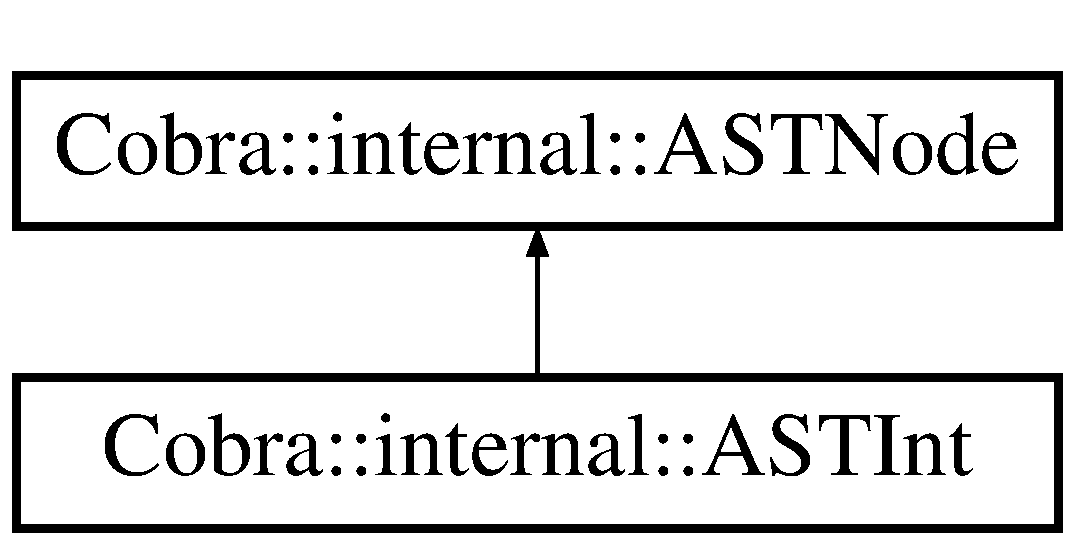
\includegraphics[height=2.000000cm]{class_cobra_1_1internal_1_1_a_s_t_int}
\end{center}
\end{figure}
\subsection*{Public Attributes}
\begin{DoxyCompactItemize}
\item 
\hypertarget{class_cobra_1_1internal_1_1_a_s_t_int_a6ef1cdf248b70931f64345d3b37c4d77}{int {\bfseries value}}\label{class_cobra_1_1internal_1_1_a_s_t_int_a6ef1cdf248b70931f64345d3b37c4d77}

\end{DoxyCompactItemize}


The documentation for this class was generated from the following file\+:\begin{DoxyCompactItemize}
\item 
src/cobra/ast/ast.\+h\end{DoxyCompactItemize}

\hypertarget{class_cobra_1_1internal_1_1_a_s_t_literary}{\section{Cobra\+:\+:internal\+:\+:A\+S\+T\+Literary Class Reference}
\label{class_cobra_1_1internal_1_1_a_s_t_literary}\index{Cobra\+::internal\+::\+A\+S\+T\+Literary@{Cobra\+::internal\+::\+A\+S\+T\+Literary}}
}
Inheritance diagram for Cobra\+:\+:internal\+:\+:A\+S\+T\+Literary\+:\begin{figure}[H]
\begin{center}
\leavevmode
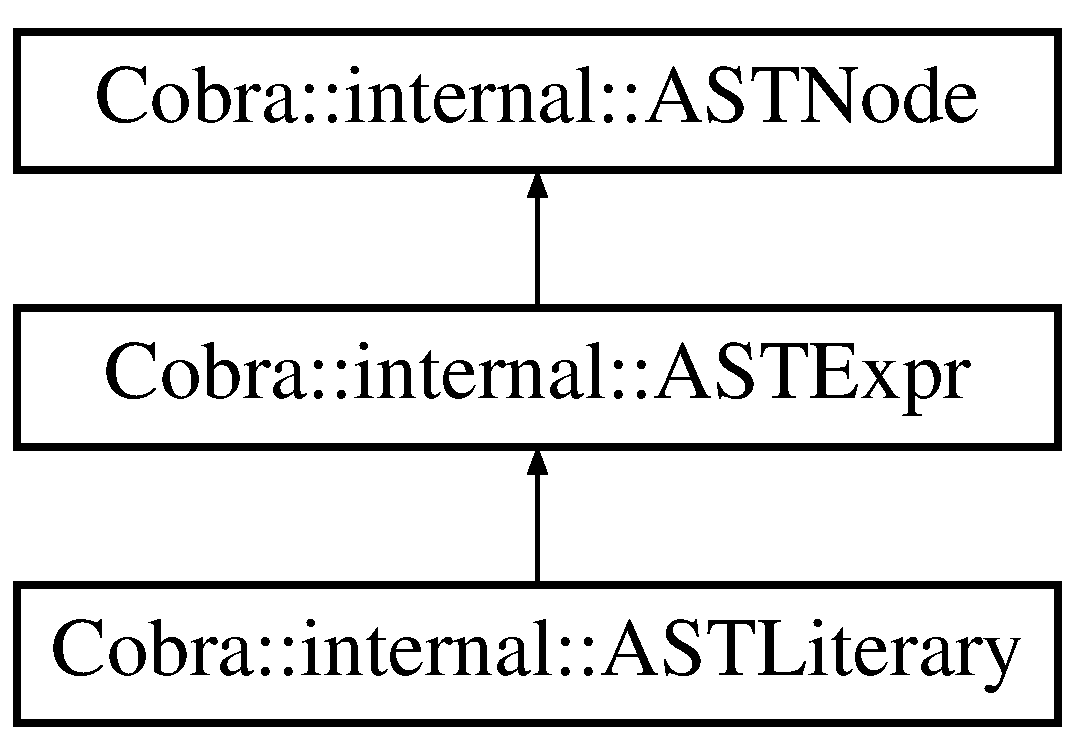
\includegraphics[height=3.000000cm]{class_cobra_1_1internal_1_1_a_s_t_literary}
\end{center}
\end{figure}
\subsection*{Public Attributes}
\begin{DoxyCompactItemize}
\item 
\hypertarget{class_cobra_1_1internal_1_1_a_s_t_literary_ab3070fdd1d7d1c311a08c66a5ee3d595}{int {\bfseries pos}}\label{class_cobra_1_1internal_1_1_a_s_t_literary_ab3070fdd1d7d1c311a08c66a5ee3d595}

\item 
\hypertarget{class_cobra_1_1internal_1_1_a_s_t_literary_a15748fbb3c828911da66b91924ca6b38}{std\+::string {\bfseries value}}\label{class_cobra_1_1internal_1_1_a_s_t_literary_a15748fbb3c828911da66b91924ca6b38}

\item 
\hypertarget{class_cobra_1_1internal_1_1_a_s_t_literary_ae73b054aee4668feebb7cfe435a5393b}{T\+O\+K\+E\+N {\bfseries kind}}\label{class_cobra_1_1internal_1_1_a_s_t_literary_ae73b054aee4668feebb7cfe435a5393b}

\end{DoxyCompactItemize}


The documentation for this class was generated from the following file\+:\begin{DoxyCompactItemize}
\item 
src/cobra/ast/ast.\+h\end{DoxyCompactItemize}

\hypertarget{class_cobra_1_1internal_1_1_a_s_t_node}{\section{Cobra\+:\+:internal\+:\+:A\+S\+T\+Node Class Reference}
\label{class_cobra_1_1internal_1_1_a_s_t_node}\index{Cobra\+::internal\+::\+A\+S\+T\+Node@{Cobra\+::internal\+::\+A\+S\+T\+Node}}
}
Inheritance diagram for Cobra\+:\+:internal\+:\+:A\+S\+T\+Node\+:\begin{figure}[H]
\begin{center}
\leavevmode
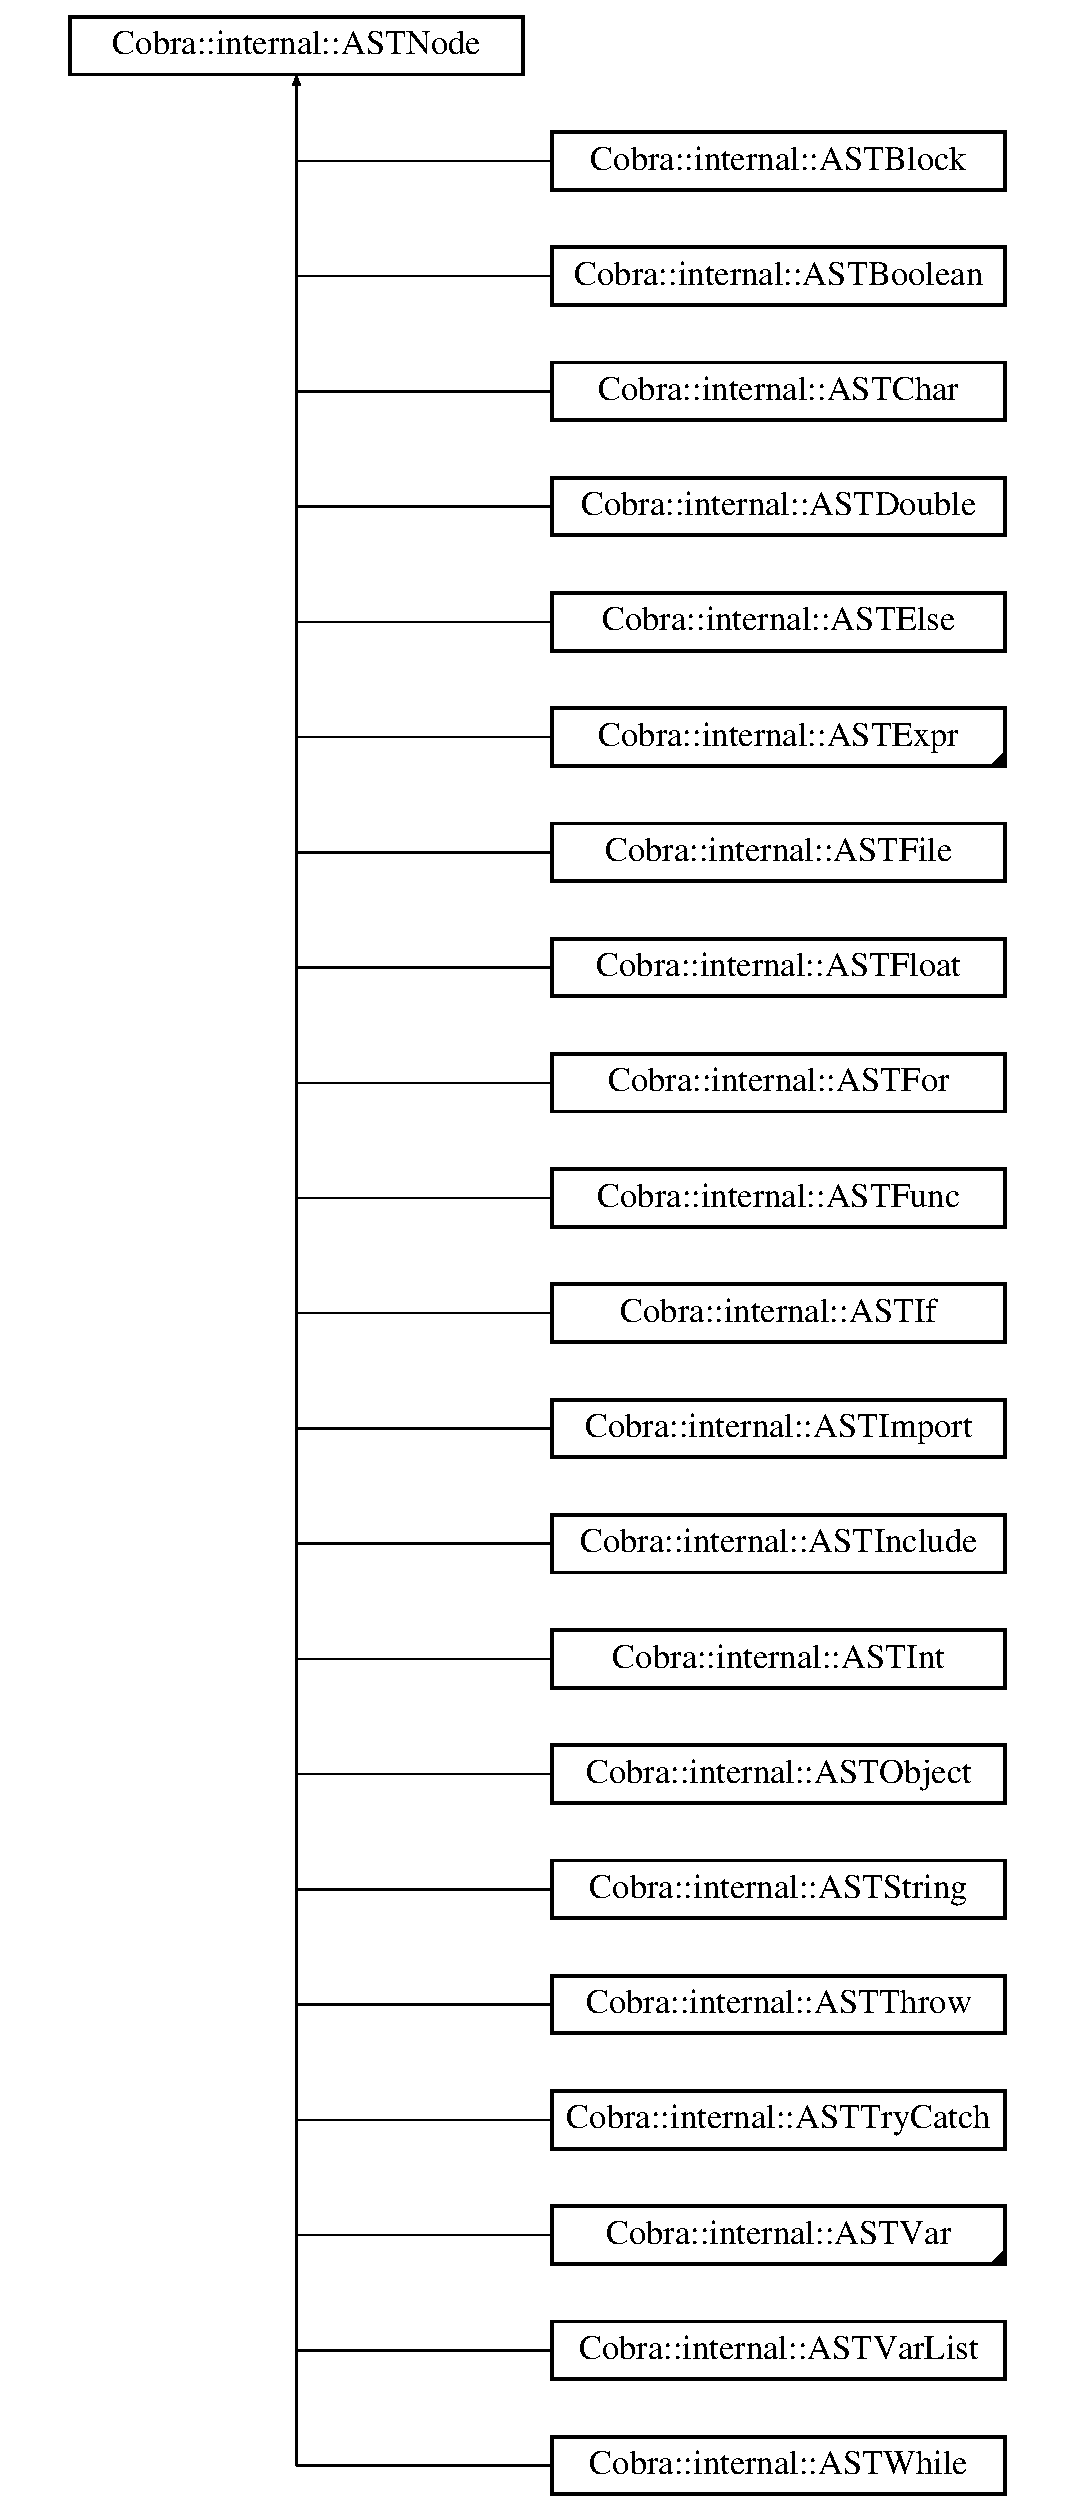
\includegraphics[height=12.000000cm]{class_cobra_1_1internal_1_1_a_s_t_node}
\end{center}
\end{figure}
\subsection*{Static Public Member Functions}
\begin{DoxyCompactItemize}
\item 
\hypertarget{class_cobra_1_1internal_1_1_a_s_t_node_af0d28a5cab4bc78d576d036b55f834f4}{static \hyperlink{class_cobra_1_1internal_1_1_a_s_t_node}{A\+S\+T\+Node} $\ast$ {\bfseries New} (\hyperlink{class_cobra_1_1internal_1_1_isolate}{Isolate} $\ast$iso)}\label{class_cobra_1_1internal_1_1_a_s_t_node_af0d28a5cab4bc78d576d036b55f834f4}

\item 
\hypertarget{class_cobra_1_1internal_1_1_a_s_t_node_a1b29f5beb1d464b2e50b57d3372f2f38}{static void {\bfseries Set\+Defaults} (\hyperlink{class_cobra_1_1internal_1_1_a_s_t_node}{A\+S\+T\+Node} $\ast$node)}\label{class_cobra_1_1internal_1_1_a_s_t_node_a1b29f5beb1d464b2e50b57d3372f2f38}

\end{DoxyCompactItemize}
\subsection*{Public Attributes}
\begin{DoxyCompactItemize}
\item 
\hypertarget{class_cobra_1_1internal_1_1_a_s_t_node_a009c5e13135b18c7475bb0bb6e1751e5}{std\+::string {\bfseries name}}\label{class_cobra_1_1internal_1_1_a_s_t_node_a009c5e13135b18c7475bb0bb6e1751e5}

\item 
\hypertarget{class_cobra_1_1internal_1_1_a_s_t_node_a94f2dac0233b841edddeeed35e768868}{T\+O\+K\+E\+N {\bfseries type}}\label{class_cobra_1_1internal_1_1_a_s_t_node_a94f2dac0233b841edddeeed35e768868}

\item 
\hypertarget{class_cobra_1_1internal_1_1_a_s_t_node_a845a463b42877638f089bd1bd2a6c973}{V\+I\+S\+I\+B\+I\+L\+I\+T\+Y {\bfseries visibility}}\label{class_cobra_1_1internal_1_1_a_s_t_node_a845a463b42877638f089bd1bd2a6c973}

\item 
\hypertarget{class_cobra_1_1internal_1_1_a_s_t_node_addf036b6ff25716a32e763328c2f4837}{bool {\bfseries scan}}\label{class_cobra_1_1internal_1_1_a_s_t_node_addf036b6ff25716a32e763328c2f4837}

\item 
\hypertarget{class_cobra_1_1internal_1_1_a_s_t_node_a4b38b68b9d85d0b2756dfb8481a92399}{int {\bfseries row}}\label{class_cobra_1_1internal_1_1_a_s_t_node_a4b38b68b9d85d0b2756dfb8481a92399}

\item 
\hypertarget{class_cobra_1_1internal_1_1_a_s_t_node_acb5d20f5ce2459ca952ac90bf825160d}{int {\bfseries col}}\label{class_cobra_1_1internal_1_1_a_s_t_node_acb5d20f5ce2459ca952ac90bf825160d}

\item 
\hypertarget{class_cobra_1_1internal_1_1_a_s_t_node_a9d670e637b5d9187f037343f9d3fffba}{bool {\bfseries used}}\label{class_cobra_1_1internal_1_1_a_s_t_node_a9d670e637b5d9187f037343f9d3fffba}

\end{DoxyCompactItemize}


The documentation for this class was generated from the following files\+:\begin{DoxyCompactItemize}
\item 
src/cobra/ast/ast.\+h\item 
src/cobra/ast/ast.\+cc\end{DoxyCompactItemize}

\hypertarget{class_cobra_1_1internal_1_1_a_s_t_object}{\section{Cobra\+:\+:internal\+:\+:A\+S\+T\+Object Class Reference}
\label{class_cobra_1_1internal_1_1_a_s_t_object}\index{Cobra\+::internal\+::\+A\+S\+T\+Object@{Cobra\+::internal\+::\+A\+S\+T\+Object}}
}
Inheritance diagram for Cobra\+:\+:internal\+:\+:A\+S\+T\+Object\+:\begin{figure}[H]
\begin{center}
\leavevmode
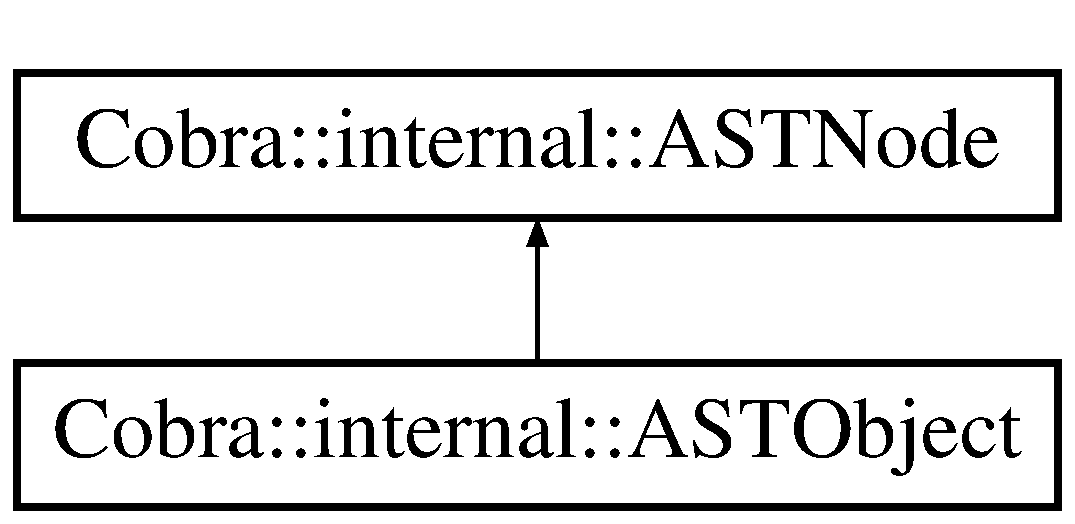
\includegraphics[height=2.000000cm]{class_cobra_1_1internal_1_1_a_s_t_object}
\end{center}
\end{figure}
\subsection*{Static Public Member Functions}
\begin{DoxyCompactItemize}
\item 
\hypertarget{class_cobra_1_1internal_1_1_a_s_t_object_a1f6c4af36fb3a5ee6cab120c7c56da2f}{static \hyperlink{class_cobra_1_1internal_1_1_a_s_t_object}{A\+S\+T\+Object} $\ast$ {\bfseries New} (\hyperlink{class_cobra_1_1internal_1_1_isolate}{Isolate} $\ast$iso)}\label{class_cobra_1_1internal_1_1_a_s_t_object_a1f6c4af36fb3a5ee6cab120c7c56da2f}

\end{DoxyCompactItemize}
\subsection*{Public Attributes}
\begin{DoxyCompactItemize}
\item 
\hypertarget{class_cobra_1_1internal_1_1_a_s_t_object_a2f905d798363fb9a9697ceeb83453cf7}{\hyperlink{class_cobra_1_1internal_1_1_vector}{Vector}$<$ \hyperlink{class_cobra_1_1internal_1_1_a_s_t_node}{A\+S\+T\+Node} $\ast$ $>$ {\bfseries members}}\label{class_cobra_1_1internal_1_1_a_s_t_object_a2f905d798363fb9a9697ceeb83453cf7}

\end{DoxyCompactItemize}


The documentation for this class was generated from the following files\+:\begin{DoxyCompactItemize}
\item 
src/cobra/ast/ast.\+h\item 
src/cobra/ast/ast.\+cc\end{DoxyCompactItemize}

\hypertarget{class_cobra_1_1internal_1_1_a_s_t_object_member_chain_expr}{\section{Cobra\+:\+:internal\+:\+:A\+S\+T\+Object\+Member\+Chain\+Expr Class Reference}
\label{class_cobra_1_1internal_1_1_a_s_t_object_member_chain_expr}\index{Cobra\+::internal\+::\+A\+S\+T\+Object\+Member\+Chain\+Expr@{Cobra\+::internal\+::\+A\+S\+T\+Object\+Member\+Chain\+Expr}}
}
Inheritance diagram for Cobra\+:\+:internal\+:\+:A\+S\+T\+Object\+Member\+Chain\+Expr\+:\begin{figure}[H]
\begin{center}
\leavevmode
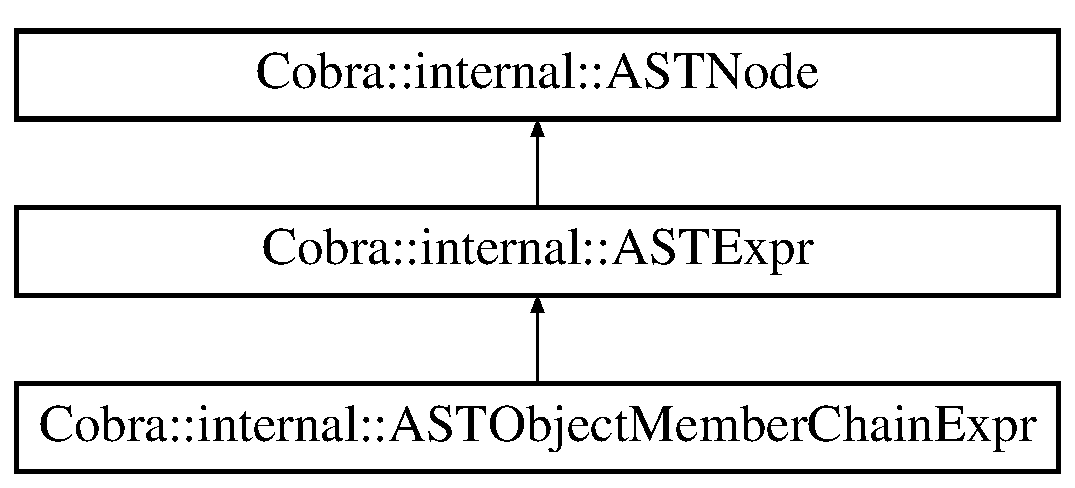
\includegraphics[height=3.000000cm]{class_cobra_1_1internal_1_1_a_s_t_object_member_chain_expr}
\end{center}
\end{figure}
\subsection*{Static Public Member Functions}
\begin{DoxyCompactItemize}
\item 
\hypertarget{class_cobra_1_1internal_1_1_a_s_t_object_member_chain_expr_afbd7d365b7a3308d61acf39bff6cd694}{static \hyperlink{class_cobra_1_1internal_1_1_a_s_t_object_member_chain_expr}{A\+S\+T\+Object\+Member\+Chain\+Expr} $\ast$ {\bfseries New} (\hyperlink{class_cobra_1_1internal_1_1_isolate}{Isolate} $\ast$iso)}\label{class_cobra_1_1internal_1_1_a_s_t_object_member_chain_expr_afbd7d365b7a3308d61acf39bff6cd694}

\end{DoxyCompactItemize}
\subsection*{Public Attributes}
\begin{DoxyCompactItemize}
\item 
\hypertarget{class_cobra_1_1internal_1_1_a_s_t_object_member_chain_expr_ab6a85fbf7191951c1de17a4208a637e7}{\hyperlink{class_cobra_1_1internal_1_1_a_s_t_expr}{A\+S\+T\+Expr} $\ast$ {\bfseries member}}\label{class_cobra_1_1internal_1_1_a_s_t_object_member_chain_expr_ab6a85fbf7191951c1de17a4208a637e7}

\item 
\hypertarget{class_cobra_1_1internal_1_1_a_s_t_object_member_chain_expr_a1198c2d503d63dec9a41f11034a59a33}{\hyperlink{class_cobra_1_1internal_1_1_a_s_t_node}{A\+S\+T\+Node} $\ast$ {\bfseries object}}\label{class_cobra_1_1internal_1_1_a_s_t_object_member_chain_expr_a1198c2d503d63dec9a41f11034a59a33}

\item 
\hypertarget{class_cobra_1_1internal_1_1_a_s_t_object_member_chain_expr_a1c21198f3672ed23e7458c1818525659}{\hyperlink{class_cobra_1_1internal_1_1_a_s_t_expr}{A\+S\+T\+Expr} $\ast$ {\bfseries value}}\label{class_cobra_1_1internal_1_1_a_s_t_object_member_chain_expr_a1c21198f3672ed23e7458c1818525659}

\item 
\hypertarget{class_cobra_1_1internal_1_1_a_s_t_object_member_chain_expr_a2c09e14e1007ea7f7e014944ef98a7c0}{bool {\bfseries is\+Setting}}\label{class_cobra_1_1internal_1_1_a_s_t_object_member_chain_expr_a2c09e14e1007ea7f7e014944ef98a7c0}

\end{DoxyCompactItemize}


The documentation for this class was generated from the following files\+:\begin{DoxyCompactItemize}
\item 
src/cobra/ast/ast.\+h\item 
src/cobra/ast/ast.\+cc\end{DoxyCompactItemize}

\hypertarget{class_cobra_1_1internal_1_1_a_s_t_string}{\section{Cobra\+:\+:internal\+:\+:A\+S\+T\+String Class Reference}
\label{class_cobra_1_1internal_1_1_a_s_t_string}\index{Cobra\+::internal\+::\+A\+S\+T\+String@{Cobra\+::internal\+::\+A\+S\+T\+String}}
}
Inheritance diagram for Cobra\+:\+:internal\+:\+:A\+S\+T\+String\+:\begin{figure}[H]
\begin{center}
\leavevmode
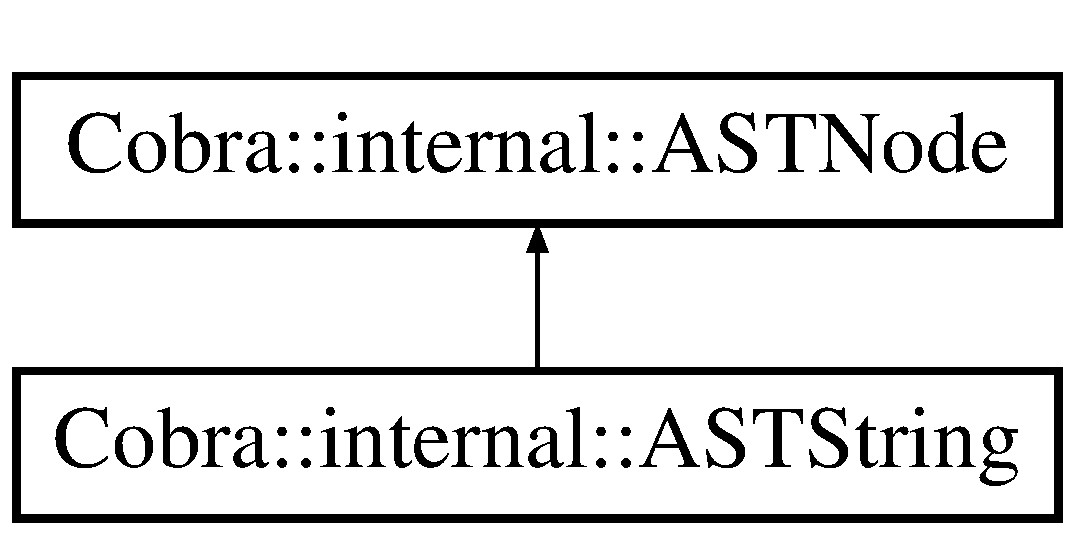
\includegraphics[height=2.000000cm]{class_cobra_1_1internal_1_1_a_s_t_string}
\end{center}
\end{figure}
\subsection*{Public Attributes}
\begin{DoxyCompactItemize}
\item 
\hypertarget{class_cobra_1_1internal_1_1_a_s_t_string_a91fd89c1cf9442e5df35d19e6fe6a465}{std\+::string {\bfseries value}}\label{class_cobra_1_1internal_1_1_a_s_t_string_a91fd89c1cf9442e5df35d19e6fe6a465}

\end{DoxyCompactItemize}


The documentation for this class was generated from the following file\+:\begin{DoxyCompactItemize}
\item 
src/cobra/ast/ast.\+h\end{DoxyCompactItemize}

\hypertarget{class_cobra_1_1internal_1_1_a_s_t_unary_expr}{\section{Cobra\+:\+:internal\+:\+:A\+S\+T\+Unary\+Expr Class Reference}
\label{class_cobra_1_1internal_1_1_a_s_t_unary_expr}\index{Cobra\+::internal\+::\+A\+S\+T\+Unary\+Expr@{Cobra\+::internal\+::\+A\+S\+T\+Unary\+Expr}}
}
Inheritance diagram for Cobra\+:\+:internal\+:\+:A\+S\+T\+Unary\+Expr\+:\begin{figure}[H]
\begin{center}
\leavevmode
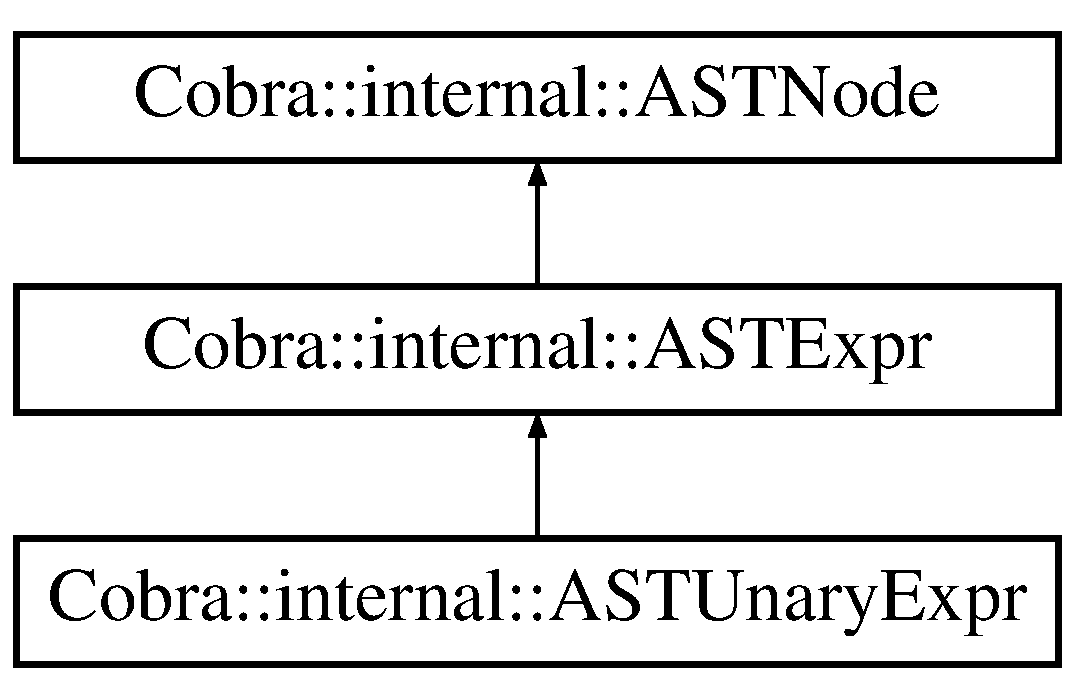
\includegraphics[height=3.000000cm]{class_cobra_1_1internal_1_1_a_s_t_unary_expr}
\end{center}
\end{figure}
\subsection*{Static Public Member Functions}
\begin{DoxyCompactItemize}
\item 
\hypertarget{class_cobra_1_1internal_1_1_a_s_t_unary_expr_a51054d2f0194a0e24ff0e54399c47c93}{static \hyperlink{class_cobra_1_1internal_1_1_a_s_t_unary_expr}{A\+S\+T\+Unary\+Expr} $\ast$ {\bfseries New} (\hyperlink{class_cobra_1_1internal_1_1_isolate}{Isolate} $\ast$iso)}\label{class_cobra_1_1internal_1_1_a_s_t_unary_expr_a51054d2f0194a0e24ff0e54399c47c93}

\end{DoxyCompactItemize}
\subsection*{Public Attributes}
\begin{DoxyCompactItemize}
\item 
\hypertarget{class_cobra_1_1internal_1_1_a_s_t_unary_expr_a42f025f4ad5154da2e8443c93b4503b6}{\hyperlink{class_cobra_1_1internal_1_1_a_s_t_expr}{A\+S\+T\+Expr} $\ast$ {\bfseries value}}\label{class_cobra_1_1internal_1_1_a_s_t_unary_expr_a42f025f4ad5154da2e8443c93b4503b6}

\item 
\hypertarget{class_cobra_1_1internal_1_1_a_s_t_unary_expr_aa284a1dd2bb9b1d09242957f322fa780}{\hyperlink{class_cobra_1_1internal_1_1_token}{Token} $\ast$ {\bfseries op}}\label{class_cobra_1_1internal_1_1_a_s_t_unary_expr_aa284a1dd2bb9b1d09242957f322fa780}

\item 
\hypertarget{class_cobra_1_1internal_1_1_a_s_t_unary_expr_aa7e66ada18fdc5b342f7b051261fde5c}{int {\bfseries pos}}\label{class_cobra_1_1internal_1_1_a_s_t_unary_expr_aa7e66ada18fdc5b342f7b051261fde5c}

\end{DoxyCompactItemize}


The documentation for this class was generated from the following files\+:\begin{DoxyCompactItemize}
\item 
src/cobra/ast/ast.\+h\item 
src/cobra/ast/ast.\+cc\end{DoxyCompactItemize}

\hypertarget{class_cobra_1_1internal_1_1_a_s_t_var}{\section{Cobra\+:\+:internal\+:\+:A\+S\+T\+Var Class Reference}
\label{class_cobra_1_1internal_1_1_a_s_t_var}\index{Cobra\+::internal\+::\+A\+S\+T\+Var@{Cobra\+::internal\+::\+A\+S\+T\+Var}}
}
Inheritance diagram for Cobra\+:\+:internal\+:\+:A\+S\+T\+Var\+:\begin{figure}[H]
\begin{center}
\leavevmode
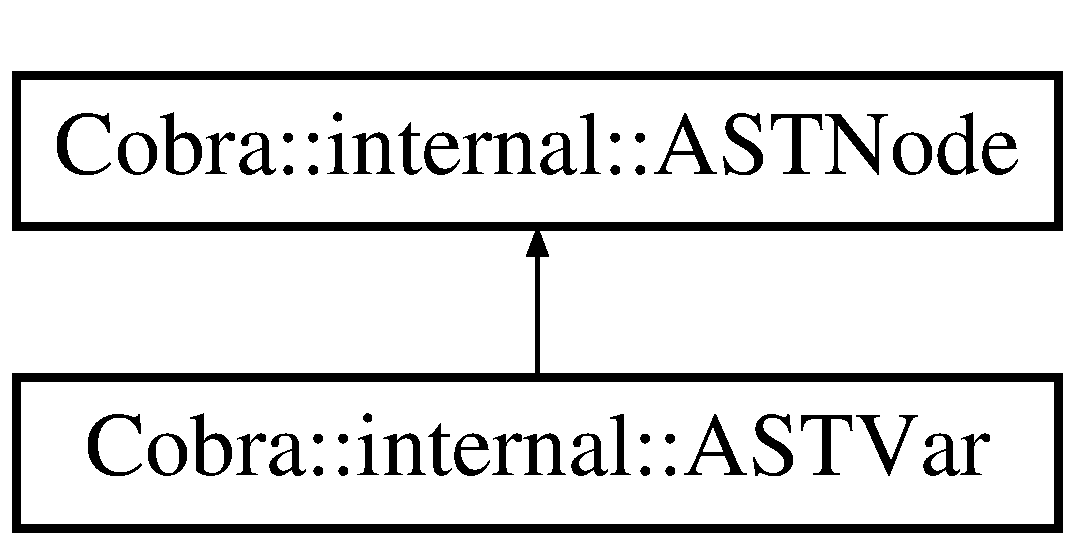
\includegraphics[height=3.000000cm]{class_cobra_1_1internal_1_1_a_s_t_var}
\end{center}
\end{figure}
\subsection*{Static Public Member Functions}
\begin{DoxyCompactItemize}
\item 
\hypertarget{class_cobra_1_1internal_1_1_a_s_t_var_a4c07624d80e9e80ff4a3311a3c47de54}{static \hyperlink{class_cobra_1_1internal_1_1_a_s_t_var}{A\+S\+T\+Var} $\ast$ {\bfseries New} (\hyperlink{class_cobra_1_1internal_1_1_isolate}{Isolate} $\ast$iso)}\label{class_cobra_1_1internal_1_1_a_s_t_var_a4c07624d80e9e80ff4a3311a3c47de54}

\end{DoxyCompactItemize}
\subsection*{Public Attributes}
\begin{DoxyCompactItemize}
\item 
\hypertarget{class_cobra_1_1internal_1_1_a_s_t_var_a92b7bdd48d6f1c52f5dc5390c7878b6c}{\hyperlink{class_cobra_1_1internal_1_1_a_s_t_expr}{A\+S\+T\+Expr} $\ast$ {\bfseries stmt}}\label{class_cobra_1_1internal_1_1_a_s_t_var_a92b7bdd48d6f1c52f5dc5390c7878b6c}

\item 
\hypertarget{class_cobra_1_1internal_1_1_a_s_t_var_a86c85537f17d498f5b0fcf15e22e76ad}{T\+O\+K\+E\+N {\bfseries var\+Type}}\label{class_cobra_1_1internal_1_1_a_s_t_var_a86c85537f17d498f5b0fcf15e22e76ad}

\item 
\hypertarget{class_cobra_1_1internal_1_1_a_s_t_var_a0e2e0adc76754328f4d85a8616daded2}{T\+O\+K\+E\+N {\bfseries array\+Type}}\label{class_cobra_1_1internal_1_1_a_s_t_var_a0e2e0adc76754328f4d85a8616daded2}

\item 
\hypertarget{class_cobra_1_1internal_1_1_a_s_t_var_ab292239765df26cb8e4ec6062d9fa4d3}{bool {\bfseries array}}\label{class_cobra_1_1internal_1_1_a_s_t_var_ab292239765df26cb8e4ec6062d9fa4d3}

\item 
\hypertarget{class_cobra_1_1internal_1_1_a_s_t_var_a6a00a268063517fbe45c2a9700f2c117}{\hyperlink{class_cobra_1_1internal_1_1_a_s_t_ident}{A\+S\+T\+Ident} $\ast$ {\bfseries var\+Class}}\label{class_cobra_1_1internal_1_1_a_s_t_var_a6a00a268063517fbe45c2a9700f2c117}

\item 
\hypertarget{class_cobra_1_1internal_1_1_a_s_t_var_a7ac1d0995a7a118ca8e1b5851c87d1e1}{bool {\bfseries cast}}\label{class_cobra_1_1internal_1_1_a_s_t_var_a7ac1d0995a7a118ca8e1b5851c87d1e1}

\item 
\hypertarget{class_cobra_1_1internal_1_1_a_s_t_var_ad330198db949f75d27f99db886889b3a}{T\+O\+K\+E\+N {\bfseries cast\+Type}}\label{class_cobra_1_1internal_1_1_a_s_t_var_ad330198db949f75d27f99db886889b3a}

\end{DoxyCompactItemize}


The documentation for this class was generated from the following files\+:\begin{DoxyCompactItemize}
\item 
src/cobra/ast/ast.\+h\item 
src/cobra/ast/ast.\+cc\end{DoxyCompactItemize}

\hypertarget{class_cobra_1_1internal_1_1_a_s_t_var_list}{\section{Cobra\+:\+:internal\+:\+:A\+S\+T\+Var\+List Class Reference}
\label{class_cobra_1_1internal_1_1_a_s_t_var_list}\index{Cobra\+::internal\+::\+A\+S\+T\+Var\+List@{Cobra\+::internal\+::\+A\+S\+T\+Var\+List}}
}
Inheritance diagram for Cobra\+:\+:internal\+:\+:A\+S\+T\+Var\+List\+:\begin{figure}[H]
\begin{center}
\leavevmode
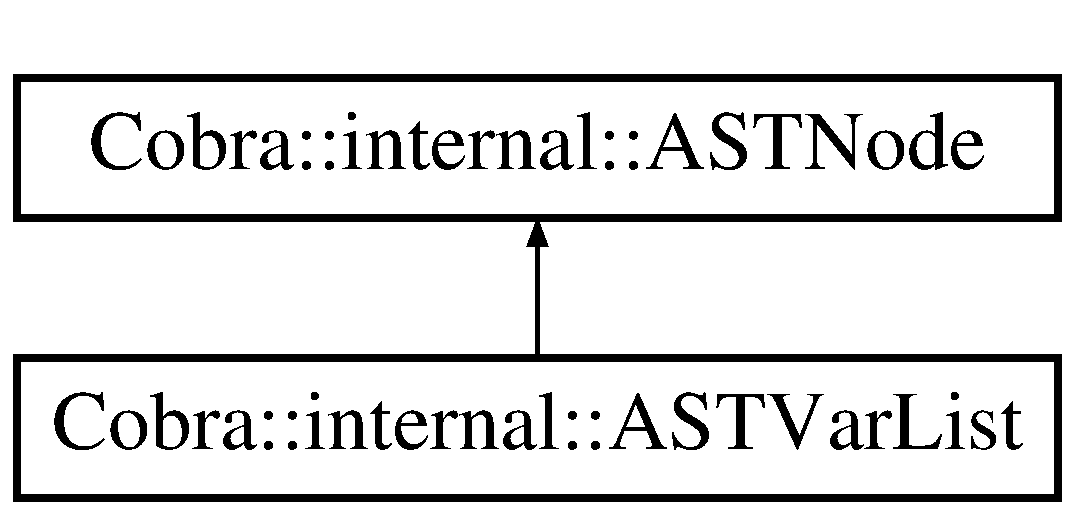
\includegraphics[height=2.000000cm]{class_cobra_1_1internal_1_1_a_s_t_var_list}
\end{center}
\end{figure}
\subsection*{Public Attributes}
\begin{DoxyCompactItemize}
\item 
\hypertarget{class_cobra_1_1internal_1_1_a_s_t_var_list_a51688944830f960f8e29e4019d46148a}{std\+::vector$<$ \hyperlink{class_cobra_1_1internal_1_1_a_s_t_var}{A\+S\+T\+Var} $\ast$ $>$ {\bfseries vars}}\label{class_cobra_1_1internal_1_1_a_s_t_var_list_a51688944830f960f8e29e4019d46148a}

\end{DoxyCompactItemize}


The documentation for this class was generated from the following file\+:\begin{DoxyCompactItemize}
\item 
src/cobra/ast/ast.\+h\end{DoxyCompactItemize}

\hypertarget{class_cobra_1_1internal_1_1_a_s_t_while}{\section{Cobra\+:\+:internal\+:\+:A\+S\+T\+While Class Reference}
\label{class_cobra_1_1internal_1_1_a_s_t_while}\index{Cobra\+::internal\+::\+A\+S\+T\+While@{Cobra\+::internal\+::\+A\+S\+T\+While}}
}
Inheritance diagram for Cobra\+:\+:internal\+:\+:A\+S\+T\+While\+:\begin{figure}[H]
\begin{center}
\leavevmode
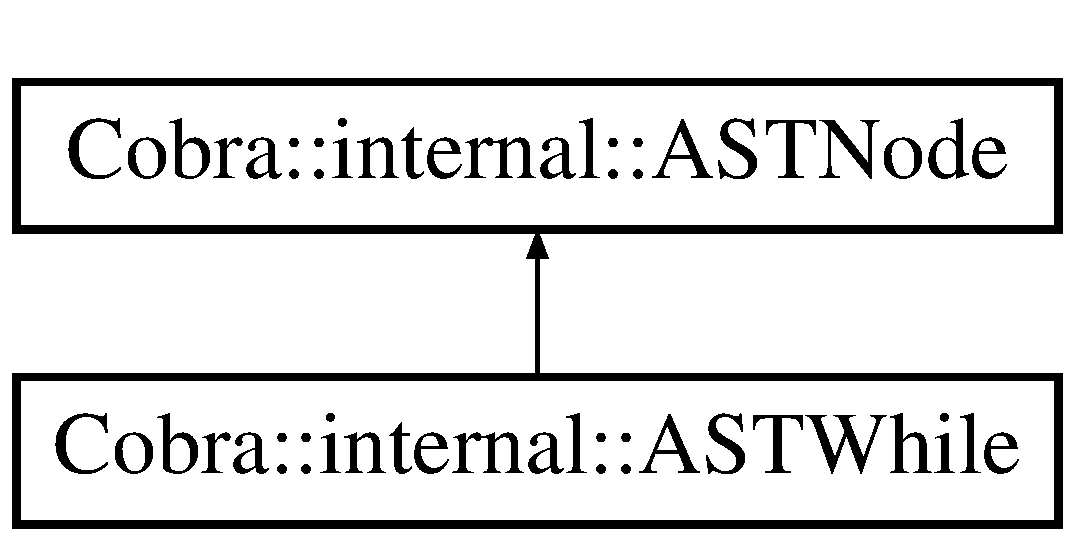
\includegraphics[height=2.000000cm]{class_cobra_1_1internal_1_1_a_s_t_while}
\end{center}
\end{figure}
\subsection*{Public Attributes}
\begin{DoxyCompactItemize}
\item 
\hypertarget{class_cobra_1_1internal_1_1_a_s_t_while_a8a97bd833a835abb8238263baa3f559b}{\hyperlink{class_cobra_1_1internal_1_1_a_s_t_expr}{A\+S\+T\+Expr} $\ast$ {\bfseries conditions}}\label{class_cobra_1_1internal_1_1_a_s_t_while_a8a97bd833a835abb8238263baa3f559b}

\item 
\hypertarget{class_cobra_1_1internal_1_1_a_s_t_while_a625f9bfdcd435fc72a6bf54cbac8984f}{\hyperlink{class_cobra_1_1internal_1_1_a_s_t_block}{A\+S\+T\+Block} $\ast$ {\bfseries block}}\label{class_cobra_1_1internal_1_1_a_s_t_while_a625f9bfdcd435fc72a6bf54cbac8984f}

\end{DoxyCompactItemize}


The documentation for this class was generated from the following file\+:\begin{DoxyCompactItemize}
\item 
src/cobra/ast/ast.\+h\end{DoxyCompactItemize}

\hypertarget{class_cobra_1_1internal_1_1_check}{\section{Cobra\+:\+:internal\+:\+:Check Class Reference}
\label{class_cobra_1_1internal_1_1_check}\index{Cobra\+::internal\+::\+Check@{Cobra\+::internal\+::\+Check}}
}
\subsection*{Public Member Functions}
\begin{DoxyCompactItemize}
\item 
\hypertarget{class_cobra_1_1internal_1_1_check_aceadf25dcbd139918ddcc751dddadaed}{void {\bfseries Check\+File} (\hyperlink{class_cobra_1_1internal_1_1_a_s_t_file}{A\+S\+T\+File} $\ast$file)}\label{class_cobra_1_1internal_1_1_check_aceadf25dcbd139918ddcc751dddadaed}

\item 
\hypertarget{class_cobra_1_1internal_1_1_check_a0221d7a96e1581a4e9c9f097c0cb75b7}{bool {\bfseries Has\+Main} ()}\label{class_cobra_1_1internal_1_1_check_a0221d7a96e1581a4e9c9f097c0cb75b7}

\item 
\hypertarget{class_cobra_1_1internal_1_1_check_afb99bd541cf71b4abc5ccfc7a583a7c2}{void {\bfseries Set\+Isolate} (\hyperlink{class_cobra_1_1internal_1_1_isolate}{Isolate} $\ast$iso)}\label{class_cobra_1_1internal_1_1_check_afb99bd541cf71b4abc5ccfc7a583a7c2}

\end{DoxyCompactItemize}
\subsection*{Public Attributes}
\begin{DoxyCompactItemize}
\item 
\hypertarget{class_cobra_1_1internal_1_1_check_a5ac845f4fe07186c2b175c5021cf3205}{int {\bfseries col}}\label{class_cobra_1_1internal_1_1_check_a5ac845f4fe07186c2b175c5021cf3205}

\item 
\hypertarget{class_cobra_1_1internal_1_1_check_aa5dab76efd3b801cd18d56b0806ca020}{int {\bfseries row}}\label{class_cobra_1_1internal_1_1_check_aa5dab76efd3b801cd18d56b0806ca020}

\end{DoxyCompactItemize}


The documentation for this class was generated from the following files\+:\begin{DoxyCompactItemize}
\item 
src/cobra/ast/check.\+h\item 
src/cobra/ast/check.\+cc\end{DoxyCompactItemize}

\hypertarget{class_cobra_1_1internal_1_1_clock}{\section{Cobra\+:\+:internal\+:\+:Clock Class Reference}
\label{class_cobra_1_1internal_1_1_clock}\index{Cobra\+::internal\+::\+Clock@{Cobra\+::internal\+::\+Clock}}
}
\subsection*{Public Member Functions}
\begin{DoxyCompactItemize}
\item 
\hypertarget{class_cobra_1_1internal_1_1_clock_a6b720b9135af9ffae9d2a1283b9e6867}{void {\bfseries Start} ()}\label{class_cobra_1_1internal_1_1_clock_a6b720b9135af9ffae9d2a1283b9e6867}

\item 
\hypertarget{class_cobra_1_1internal_1_1_clock_ae9829bc4afa5a59007ea88bd2f0d54bf}{void {\bfseries Stop} ()}\label{class_cobra_1_1internal_1_1_clock_ae9829bc4afa5a59007ea88bd2f0d54bf}

\item 
\hypertarget{class_cobra_1_1internal_1_1_clock_ad6abe06abf100cd64c6b61ac450686cd}{void {\bfseries Reset} ()}\label{class_cobra_1_1internal_1_1_clock_ad6abe06abf100cd64c6b61ac450686cd}

\item 
\hypertarget{class_cobra_1_1internal_1_1_clock_a337417db217baf41dc732b537dae1ec2}{double {\bfseries Get\+Duration} ()}\label{class_cobra_1_1internal_1_1_clock_a337417db217baf41dc732b537dae1ec2}

\end{DoxyCompactItemize}


The documentation for this class was generated from the following files\+:\begin{DoxyCompactItemize}
\item 
src/cobra/clock.\+h\item 
src/cobra/clock.\+cc\end{DoxyCompactItemize}

\hypertarget{class_cobra_1_1internal_1_1_code_gen}{\section{Cobra\+:\+:internal\+:\+:Code\+Gen Class Reference}
\label{class_cobra_1_1internal_1_1_code_gen}\index{Cobra\+::internal\+::\+Code\+Gen@{Cobra\+::internal\+::\+Code\+Gen}}
}
\subsection*{Public Member Functions}
\begin{DoxyCompactItemize}
\item 
\hypertarget{class_cobra_1_1internal_1_1_code_gen_a084903d115ad7cf678de8a3ca5b4323a}{{\bfseries Code\+Gen} (\hyperlink{class_cobra_1_1internal_1_1_context}{Context} $\ast$context)}\label{class_cobra_1_1internal_1_1_code_gen_a084903d115ad7cf678de8a3ca5b4323a}

\end{DoxyCompactItemize}


The documentation for this class was generated from the following files\+:\begin{DoxyCompactItemize}
\item 
src/cobra/codegen/codegen.\+h\item 
src/cobra/codegen/codegen.\+cc\end{DoxyCompactItemize}

\hypertarget{class_cobra_1_1internal_1_1_context}{\section{Cobra\+:\+:internal\+:\+:Context Class Reference}
\label{class_cobra_1_1internal_1_1_context}\index{Cobra\+::internal\+::\+Context@{Cobra\+::internal\+::\+Context}}
}
\subsection*{Public Member Functions}
\begin{DoxyCompactItemize}
\item 
\hypertarget{class_cobra_1_1internal_1_1_context_a9ce99f725452c20315f88c9fb0328baa}{void {\bfseries Set\+Isolate} (\hyperlink{class_cobra_1_1internal_1_1_isolate}{Isolate} $\ast$isolate)}\label{class_cobra_1_1internal_1_1_context_a9ce99f725452c20315f88c9fb0328baa}

\item 
\hypertarget{class_cobra_1_1internal_1_1_context_a077c432927bd36374978cf56c55b58e2}{void {\bfseries Add\+Script} (\hyperlink{class_cobra_1_1internal_1_1_script}{Script} $\ast$script)}\label{class_cobra_1_1internal_1_1_context_a077c432927bd36374978cf56c55b58e2}

\item 
\hypertarget{class_cobra_1_1internal_1_1_context_a9128b4d12daae36ec57607d9d7867f6c}{\hyperlink{class_cobra_1_1internal_1_1_script}{Script} $\ast$ {\bfseries Get\+Script\+By\+String} (\hyperlink{class_cobra_1_1internal_1_1_isolate}{Isolate} $\ast$iso, std\+::string code)}\label{class_cobra_1_1internal_1_1_context_a9128b4d12daae36ec57607d9d7867f6c}

\item 
\hypertarget{class_cobra_1_1internal_1_1_context_a2309f31e215ee3278600c9b057fc7317}{bool {\bfseries Is\+Included} (\hyperlink{class_cobra_1_1internal_1_1_isolate}{Isolate} $\ast$iso, const char $\ast$path)}\label{class_cobra_1_1internal_1_1_context_a2309f31e215ee3278600c9b057fc7317}

\item 
\hypertarget{class_cobra_1_1internal_1_1_context_a6392369b035385205d537719d3ebea22}{bool {\bfseries Is\+Imported} (\hyperlink{class_cobra_1_1internal_1_1_isolate}{Isolate} $\ast$iso, std\+::string name)}\label{class_cobra_1_1internal_1_1_context_a6392369b035385205d537719d3ebea22}

\item 
\hypertarget{class_cobra_1_1internal_1_1_context_ac604a6bd9357f93c0d3e49b725305350}{void {\bfseries Set\+Import} (std\+::string name)}\label{class_cobra_1_1internal_1_1_context_ac604a6bd9357f93c0d3e49b725305350}

\item 
\hypertarget{class_cobra_1_1internal_1_1_context_a28c2f40e6d64392b412184212005645c}{void {\bfseries Add\+To\+In\+Progress} (std\+::string str)}\label{class_cobra_1_1internal_1_1_context_a28c2f40e6d64392b412184212005645c}

\item 
\hypertarget{class_cobra_1_1internal_1_1_context_afe6bf704c553475cbdc32d89e489a852}{void {\bfseries Remove\+From\+In\+Progress} (std\+::string str)}\label{class_cobra_1_1internal_1_1_context_afe6bf704c553475cbdc32d89e489a852}

\item 
\hypertarget{class_cobra_1_1internal_1_1_context_ac5fbe95bc5050c2d65e1613b8ee394ee}{\hyperlink{class_cobra_1_1internal_1_1_a_s_t_node}{A\+S\+T\+Node} $\ast$ {\bfseries Get\+Exported\+Node} (\hyperlink{class_cobra_1_1internal_1_1_isolate}{Isolate} $\ast$iso, std\+::string name)}\label{class_cobra_1_1internal_1_1_context_ac5fbe95bc5050c2d65e1613b8ee394ee}

\item 
\hypertarget{class_cobra_1_1internal_1_1_context_a4c9a29cfb706daa42c584f21d1c2f881}{void {\bfseries Print\+Exported} (\hyperlink{class_cobra_1_1internal_1_1_isolate}{Isolate} $\ast$iso)}\label{class_cobra_1_1internal_1_1_context_a4c9a29cfb706daa42c584f21d1c2f881}

\end{DoxyCompactItemize}


The documentation for this class was generated from the following files\+:\begin{DoxyCompactItemize}
\item 
src/cobra/ast/context.\+h\item 
src/cobra/ast/context.\+cc\end{DoxyCompactItemize}

\hypertarget{class_cobra_1_1_context}{\section{Cobra\+:\+:Context Class Reference}
\label{class_cobra_1_1_context}\index{Cobra\+::\+Context@{Cobra\+::\+Context}}
}


Creates the context for the program.  




{\ttfamily \#include $<$Cobra.\+h$>$}

\subsection*{Public Member Functions}
\begin{DoxyCompactItemize}
\item 
void $\ast$ \hyperlink{class_cobra_1_1_context_ac34fa8ed39938076d0441adabcbc1cd5}{operator new} (size\+\_\+t)
\begin{DoxyCompactList}\small\item\em Create a new context. \end{DoxyCompactList}\item 
\hypertarget{class_cobra_1_1_context_ab0c0a9a4910865623f0c89b298609f48}{void {\bfseries Set\+Isolate} (\hyperlink{class_cobra_1_1_isolate}{Isolate} $\ast$isolate)}\label{class_cobra_1_1_context_ab0c0a9a4910865623f0c89b298609f48}

\end{DoxyCompactItemize}
\subsection*{Static Public Member Functions}
\begin{DoxyCompactItemize}
\item 
static \hyperlink{class_cobra_1_1_context}{Context} $\ast$ \hyperlink{class_cobra_1_1_context_af5e66888a00a8e0f350e603c2ccbfe9d}{New} ()
\begin{DoxyCompactList}\small\item\em Create a new \hyperlink{class_cobra_1_1_context}{Cobra\+::\+Context}. \end{DoxyCompactList}\end{DoxyCompactItemize}


\subsection{Detailed Description}
Creates the context for the program. 

Global variables, functions, objects, etc... can't extend past the context. 

\subsection{Member Function Documentation}
\hypertarget{class_cobra_1_1_context_af5e66888a00a8e0f350e603c2ccbfe9d}{\index{Cobra\+::\+Context@{Cobra\+::\+Context}!New@{New}}
\index{New@{New}!Cobra\+::\+Context@{Cobra\+::\+Context}}
\subsubsection[{New}]{\setlength{\rightskip}{0pt plus 5cm}{\bf Context} $\ast$ Cobra\+::\+Context\+::\+New (
\begin{DoxyParamCaption}
{}
\end{DoxyParamCaption}
)\hspace{0.3cm}{\ttfamily [static]}}}\label{class_cobra_1_1_context_af5e66888a00a8e0f350e603c2ccbfe9d}


Create a new \hyperlink{class_cobra_1_1_context}{Cobra\+::\+Context}. 

\begin{DoxyReturn}{Returns}
\hyperlink{class_cobra_1_1_context}{Cobra\+::\+Context} 
\end{DoxyReturn}
\hypertarget{class_cobra_1_1_context_ac34fa8ed39938076d0441adabcbc1cd5}{\index{Cobra\+::\+Context@{Cobra\+::\+Context}!operator new@{operator new}}
\index{operator new@{operator new}!Cobra\+::\+Context@{Cobra\+::\+Context}}
\subsubsection[{operator new}]{\setlength{\rightskip}{0pt plus 5cm}void $\ast$ Cobra\+::\+Context\+::operator new (
\begin{DoxyParamCaption}
\item[{size\+\_\+t}]{size}
\end{DoxyParamCaption}
)}}\label{class_cobra_1_1_context_ac34fa8ed39938076d0441adabcbc1cd5}


Create a new context. 

the \char`\"{}new\char`\"{} keyword calls \hyperlink{class_cobra_1_1_context_af5e66888a00a8e0f350e603c2ccbfe9d}{Context\+::\+New()};


\begin{DoxyParams}{Parameters}
{\em size} & Unused but required \\
\hline
\end{DoxyParams}
\begin{DoxyReturn}{Returns}
\hyperlink{class_cobra_1_1_context}{Cobra\+::\+Context} 
\end{DoxyReturn}


The documentation for this class was generated from the following files\+:\begin{DoxyCompactItemize}
\item 
include/Cobra.\+h\item 
src/api.\+cc\end{DoxyCompactItemize}

\hypertarget{class_cobra_1_1internal_1_1_factory}{\section{Cobra\+:\+:internal\+:\+:Factory Class Reference}
\label{class_cobra_1_1internal_1_1_factory}\index{Cobra\+::internal\+::\+Factory@{Cobra\+::internal\+::\+Factory}}
}
\subsection*{Public Member Functions}
\begin{DoxyCompactItemize}
\item 
\hypertarget{class_cobra_1_1internal_1_1_factory_a8b645b10420d689716ebfb307ff047d1}{\hyperlink{class_cobra_1_1internal_1_1_string}{String} $\ast$ {\bfseries New\+String} (const char $\ast$str)}\label{class_cobra_1_1internal_1_1_factory_a8b645b10420d689716ebfb307ff047d1}

\item 
\hypertarget{class_cobra_1_1internal_1_1_factory_aed7a84a295acae0539dd765e35842f1a}{\hyperlink{class_cobra_1_1internal_1_1_script}{Script} $\ast$ {\bfseries New\+Script} (\hyperlink{class_cobra_1_1internal_1_1_handle}{Handle} $\ast$handle)}\label{class_cobra_1_1internal_1_1_factory_aed7a84a295acae0539dd765e35842f1a}

\end{DoxyCompactItemize}


The documentation for this class was generated from the following files\+:\begin{DoxyCompactItemize}
\item 
src/cobra/mem/factory.\+h\item 
src/cobra/mem/factory.\+cc\end{DoxyCompactItemize}

\hypertarget{class_cobra_1_1internal_1_1_flags}{\section{Cobra\+:\+:internal\+:\+:Flags Class Reference}
\label{class_cobra_1_1internal_1_1_flags}\index{Cobra\+::internal\+::\+Flags@{Cobra\+::internal\+::\+Flags}}
}
\subsection*{Static Public Member Functions}
\begin{DoxyCompactItemize}
\item 
\hypertarget{class_cobra_1_1internal_1_1_flags_a74931598fb17cee698b27975c5feda6e}{static void {\bfseries Set\+Command\+Line\+Flags} (int argc, const char $\ast$argv\mbox{[}$\,$\mbox{]})}\label{class_cobra_1_1internal_1_1_flags_a74931598fb17cee698b27975c5feda6e}

\end{DoxyCompactItemize}
\subsection*{Static Public Attributes}
\begin{DoxyCompactItemize}
\item 
\hypertarget{class_cobra_1_1internal_1_1_flags_ac08d43fe0936cb71bfee597af803dbe2}{static bool {\bfseries trace\+Parser} = false}\label{class_cobra_1_1internal_1_1_flags_ac08d43fe0936cb71bfee597af803dbe2}

\item 
\hypertarget{class_cobra_1_1internal_1_1_flags_a7181e6f3330ab86bff83a6520c74901e}{static bool {\bfseries trace\+Check} = false}\label{class_cobra_1_1internal_1_1_flags_a7181e6f3330ab86bff83a6520c74901e}

\item 
\hypertarget{class_cobra_1_1internal_1_1_flags_ae050100f3071586aebd9a89ec44db04f}{static bool {\bfseries print\+Variables} = false}\label{class_cobra_1_1internal_1_1_flags_ae050100f3071586aebd9a89ec44db04f}

\item 
\hypertarget{class_cobra_1_1internal_1_1_flags_afa0e8679e4526d6edbe06b935da2c4da}{static bool {\bfseries parsing\+Time} = false}\label{class_cobra_1_1internal_1_1_flags_afa0e8679e4526d6edbe06b935da2c4da}

\item 
\hypertarget{class_cobra_1_1internal_1_1_flags_ae77a4d0d2533d664c6234789401ae0fe}{static bool {\bfseries heap\+Insert} = false}\label{class_cobra_1_1internal_1_1_flags_ae77a4d0d2533d664c6234789401ae0fe}

\item 
\hypertarget{class_cobra_1_1internal_1_1_flags_a80d0f082f3e0ea5a10ef9da3ef3d45ed}{static bool {\bfseries heap\+Delete} = false}\label{class_cobra_1_1internal_1_1_flags_a80d0f082f3e0ea5a10ef9da3ef3d45ed}

\item 
\hypertarget{class_cobra_1_1internal_1_1_flags_a1eacd9c9fcaed39873b051cbca8f9424}{static bool {\bfseries exported\+Nodes} = false}\label{class_cobra_1_1internal_1_1_flags_a1eacd9c9fcaed39873b051cbca8f9424}

\item 
\hypertarget{class_cobra_1_1internal_1_1_flags_a14a2af40fa06fc5f063561ffb7497aa4}{static bool {\bfseries memory\+Audit} = false}\label{class_cobra_1_1internal_1_1_flags_a14a2af40fa06fc5f063561ffb7497aa4}

\item 
\hypertarget{class_cobra_1_1internal_1_1_flags_a2ecc52907c7e5aa767258d4aae11f23e}{static bool {\bfseries memory\+Request} = false}\label{class_cobra_1_1internal_1_1_flags_a2ecc52907c7e5aa767258d4aae11f23e}

\end{DoxyCompactItemize}


The documentation for this class was generated from the following files\+:\begin{DoxyCompactItemize}
\item 
src/cobra/flags.\+h\item 
src/cobra/flags.\+cc\end{DoxyCompactItemize}

\hypertarget{class_cobra_1_1internal_1_1_handle}{\section{Cobra\+:\+:internal\+:\+:Handle Class Reference}
\label{class_cobra_1_1internal_1_1_handle}\index{Cobra\+::internal\+::\+Handle@{Cobra\+::internal\+::\+Handle}}
}
\subsection*{Public Member Functions}
\begin{DoxyCompactItemize}
\item 
\hypertarget{class_cobra_1_1internal_1_1_handle_a0d9840ec9a102d4e600257ee4cfd1269}{{\bfseries Handle} (\hyperlink{struct_cobra_1_1internal_1_1_heap_object}{Heap\+Object} $\ast$o=N\+U\+L\+L, \hyperlink{class_cobra_1_1internal_1_1_isolate}{Isolate} $\ast$iso=N\+U\+L\+L)}\label{class_cobra_1_1internal_1_1_handle_a0d9840ec9a102d4e600257ee4cfd1269}

\item 
\hypertarget{class_cobra_1_1internal_1_1_handle_a73e7eec02b0364ff8b93d058262858f9}{\hyperlink{struct_cobra_1_1internal_1_1_heap_object}{Heap\+Object} $\ast$ {\bfseries Get\+Object} ()}\label{class_cobra_1_1internal_1_1_handle_a73e7eec02b0364ff8b93d058262858f9}

\item 
\hypertarget{class_cobra_1_1internal_1_1_handle_ab41a1526137640b18e2c6f2da297a80a}{\hyperlink{class_cobra_1_1internal_1_1_string}{String} $\ast$ {\bfseries To\+String} ()}\label{class_cobra_1_1internal_1_1_handle_ab41a1526137640b18e2c6f2da297a80a}

\item 
\hypertarget{class_cobra_1_1internal_1_1_handle_a8373f2edb1922a2da2c5b62ae6f700af}{\hyperlink{class_cobra_1_1internal_1_1_script}{Script} $\ast$ {\bfseries To\+Script} ()}\label{class_cobra_1_1internal_1_1_handle_a8373f2edb1922a2da2c5b62ae6f700af}

\end{DoxyCompactItemize}
\subsection*{Static Public Member Functions}
\begin{DoxyCompactItemize}
\item 
\hypertarget{class_cobra_1_1internal_1_1_handle_a443c0ea101538de9670b8610f51dd5e5}{static bool {\bfseries Is\+Address\+Valid} (\hyperlink{class_cobra_1_1internal_1_1_isolate}{Isolate} $\ast$iso, Address addr)}\label{class_cobra_1_1internal_1_1_handle_a443c0ea101538de9670b8610f51dd5e5}

\item 
\hypertarget{class_cobra_1_1internal_1_1_handle_a5ff8948c170fe906766690b7e5cb3388}{static \hyperlink{class_cobra_1_1internal_1_1_handle}{Handle} $\ast$ {\bfseries New} (\hyperlink{struct_cobra_1_1internal_1_1_heap_object}{Heap\+Object} $\ast$o=N\+U\+L\+L, \hyperlink{class_cobra_1_1internal_1_1_isolate}{Isolate} $\ast$iso=N\+U\+L\+L)}\label{class_cobra_1_1internal_1_1_handle_a5ff8948c170fe906766690b7e5cb3388}

\end{DoxyCompactItemize}
\subsection*{Public Attributes}
\begin{DoxyCompactItemize}
\item 
\hypertarget{class_cobra_1_1internal_1_1_handle_a1e0b8e3eeffa8d7e9fd85ae2f3559aa7}{\hyperlink{class_cobra_1_1internal_1_1_isolate}{Isolate} $\ast$ {\bfseries isolate}}\label{class_cobra_1_1internal_1_1_handle_a1e0b8e3eeffa8d7e9fd85ae2f3559aa7}

\end{DoxyCompactItemize}


The documentation for this class was generated from the following files\+:\begin{DoxyCompactItemize}
\item 
src/cobra/mem/handle.\+h\item 
src/cobra/mem/handle.\+cc\end{DoxyCompactItemize}

\hypertarget{class_cobra_1_1_handle}{\section{Cobra\+:\+:Handle Class Reference}
\label{class_cobra_1_1_handle}\index{Cobra\+::\+Handle@{Cobra\+::\+Handle}}
}


All \hyperlink{namespace_cobra}{Cobra} scripts and objects will be wrapped in a handler.  




{\ttfamily \#include $<$Cobra.\+h$>$}

\subsection*{Public Member Functions}
\begin{DoxyCompactItemize}
\item 
bool \hyperlink{class_cobra_1_1_handle_a1cd39727327efaaea04597acae87eca7}{Is\+String} ()
\begin{DoxyCompactList}\small\item\em \hyperlink{class_cobra_1_1_handle}{Handle} is \hyperlink{class_cobra_1_1_string}{String}. \end{DoxyCompactList}\item 
bool \hyperlink{class_cobra_1_1_handle_a4e641103844a622cec39b8e53f056112}{Is\+Script} ()
\begin{DoxyCompactList}\small\item\em \hyperlink{class_cobra_1_1_handle}{Handle} is \hyperlink{class_cobra_1_1_script}{Script}. \end{DoxyCompactList}\item 
const char $\ast$ \hyperlink{class_cobra_1_1_handle_a1cc4baae13a1fbf6d5d101b5fc5b11d5}{To\+String} ()
\begin{DoxyCompactList}\small\item\em Stringify the \hyperlink{class_cobra_1_1_handle}{Handle} object. \end{DoxyCompactList}\item 
const char $\ast$ \hyperlink{class_cobra_1_1_handle_a638691042734265cab9b15668fd72fc8}{Get\+Type} ()
\begin{DoxyCompactList}\small\item\em Get the type of the \hyperlink{class_cobra_1_1_handle}{Handle}. \end{DoxyCompactList}\item 
void \hyperlink{class_cobra_1_1_handle_a8315ff0b3b5abb81ca24f987cf81b6a8}{Run} ()
\begin{DoxyCompactList}\small\item\em Runs the script. \end{DoxyCompactList}\end{DoxyCompactItemize}


\subsection{Detailed Description}
All \hyperlink{namespace_cobra}{Cobra} scripts and objects will be wrapped in a handler. 

The handler is used to hold the memory location of the object. This allows for the garbage collector to track each object. 

\subsection{Member Function Documentation}
\hypertarget{class_cobra_1_1_handle_a638691042734265cab9b15668fd72fc8}{\index{Cobra\+::\+Handle@{Cobra\+::\+Handle}!Get\+Type@{Get\+Type}}
\index{Get\+Type@{Get\+Type}!Cobra\+::\+Handle@{Cobra\+::\+Handle}}
\subsubsection[{Get\+Type}]{\setlength{\rightskip}{0pt plus 5cm}const char $\ast$ Cobra\+::\+Handle\+::\+Get\+Type (
\begin{DoxyParamCaption}
{}
\end{DoxyParamCaption}
)}}\label{class_cobra_1_1_handle_a638691042734265cab9b15668fd72fc8}


Get the type of the \hyperlink{class_cobra_1_1_handle}{Handle}. 

\begin{DoxyReturn}{Returns}
const char$\ast$ 
\end{DoxyReturn}
\hypertarget{class_cobra_1_1_handle_a4e641103844a622cec39b8e53f056112}{\index{Cobra\+::\+Handle@{Cobra\+::\+Handle}!Is\+Script@{Is\+Script}}
\index{Is\+Script@{Is\+Script}!Cobra\+::\+Handle@{Cobra\+::\+Handle}}
\subsubsection[{Is\+Script}]{\setlength{\rightskip}{0pt plus 5cm}bool Cobra\+::\+Handle\+::\+Is\+Script (
\begin{DoxyParamCaption}
{}
\end{DoxyParamCaption}
)}}\label{class_cobra_1_1_handle_a4e641103844a622cec39b8e53f056112}


\hyperlink{class_cobra_1_1_handle}{Handle} is \hyperlink{class_cobra_1_1_script}{Script}. 

Checks if the contents of the \hyperlink{class_cobra_1_1_handle}{Handle} is a \hyperlink{class_cobra_1_1_script}{Cobra\+::\+Script} \begin{DoxyReturn}{Returns}
bool 
\end{DoxyReturn}
\hypertarget{class_cobra_1_1_handle_a1cd39727327efaaea04597acae87eca7}{\index{Cobra\+::\+Handle@{Cobra\+::\+Handle}!Is\+String@{Is\+String}}
\index{Is\+String@{Is\+String}!Cobra\+::\+Handle@{Cobra\+::\+Handle}}
\subsubsection[{Is\+String}]{\setlength{\rightskip}{0pt plus 5cm}bool Cobra\+::\+Handle\+::\+Is\+String (
\begin{DoxyParamCaption}
{}
\end{DoxyParamCaption}
)}}\label{class_cobra_1_1_handle_a1cd39727327efaaea04597acae87eca7}


\hyperlink{class_cobra_1_1_handle}{Handle} is \hyperlink{class_cobra_1_1_string}{String}. 

Checks if the contents of the \hyperlink{class_cobra_1_1_handle}{Handle} is a \hyperlink{class_cobra_1_1_string}{Cobra\+::\+String}. \begin{DoxyReturn}{Returns}
bool 
\end{DoxyReturn}
\hypertarget{class_cobra_1_1_handle_a8315ff0b3b5abb81ca24f987cf81b6a8}{\index{Cobra\+::\+Handle@{Cobra\+::\+Handle}!Run@{Run}}
\index{Run@{Run}!Cobra\+::\+Handle@{Cobra\+::\+Handle}}
\subsubsection[{Run}]{\setlength{\rightskip}{0pt plus 5cm}void Cobra\+::\+Handle\+::\+Run (
\begin{DoxyParamCaption}
{}
\end{DoxyParamCaption}
)}}\label{class_cobra_1_1_handle_a8315ff0b3b5abb81ca24f987cf81b6a8}


Runs the script. 

This executes the code, compiles and runs all the imports \hypertarget{class_cobra_1_1_handle_a1cc4baae13a1fbf6d5d101b5fc5b11d5}{\index{Cobra\+::\+Handle@{Cobra\+::\+Handle}!To\+String@{To\+String}}
\index{To\+String@{To\+String}!Cobra\+::\+Handle@{Cobra\+::\+Handle}}
\subsubsection[{To\+String}]{\setlength{\rightskip}{0pt plus 5cm}const char $\ast$ Cobra\+::\+Handle\+::\+To\+String (
\begin{DoxyParamCaption}
{}
\end{DoxyParamCaption}
)}}\label{class_cobra_1_1_handle_a1cc4baae13a1fbf6d5d101b5fc5b11d5}


Stringify the \hyperlink{class_cobra_1_1_handle}{Handle} object. 

If the contents of the Hanle is a \hyperlink{class_cobra_1_1_string}{Cobra\+::\+String}, the const char$\ast$ value will be returned. \begin{DoxyReturn}{Returns}
const char$\ast$ 
\end{DoxyReturn}


The documentation for this class was generated from the following files\+:\begin{DoxyCompactItemize}
\item 
include/Cobra.\+h\item 
src/api.\+cc\end{DoxyCompactItemize}

\hypertarget{class_cobra_1_1internal_1_1_heap}{\section{Cobra\+:\+:internal\+:\+:Heap Class Reference}
\label{class_cobra_1_1internal_1_1_heap}\index{Cobra\+::internal\+::\+Heap@{Cobra\+::internal\+::\+Heap}}
}
\subsection*{Public Member Functions}
\begin{DoxyCompactItemize}
\item 
\hypertarget{class_cobra_1_1internal_1_1_heap_aabea35e11b9ad9bb9d90b1c027424396}{\hyperlink{struct_cobra_1_1internal_1_1_heap_object}{Heap\+Object} $\ast$ {\bfseries Get} (int idx)}\label{class_cobra_1_1internal_1_1_heap_aabea35e11b9ad9bb9d90b1c027424396}

\item 
\hypertarget{class_cobra_1_1internal_1_1_heap_a42859090edacdd5de263e27711a9eca6}{int {\bfseries Size} ()}\label{class_cobra_1_1internal_1_1_heap_a42859090edacdd5de263e27711a9eca6}

\item 
\hypertarget{class_cobra_1_1internal_1_1_heap_a6110bb56a06dd1873c884c254f87d60e}{\hyperlink{struct_cobra_1_1internal_1_1_heap_object}{Heap\+Object} $\ast$ {\bfseries Insert} (\hyperlink{struct_cobra_1_1internal_1_1_heap_object}{Heap\+Object} val)}\label{class_cobra_1_1internal_1_1_heap_a6110bb56a06dd1873c884c254f87d60e}

\item 
\hypertarget{class_cobra_1_1internal_1_1_heap_a0d8e49caa6e2a2c7e734fcea54e9b19d}{bool {\bfseries Delete} (int idx)}\label{class_cobra_1_1internal_1_1_heap_a0d8e49caa6e2a2c7e734fcea54e9b19d}

\end{DoxyCompactItemize}


The documentation for this class was generated from the following file\+:\begin{DoxyCompactItemize}
\item 
src/cobra/mem/heap.\+h\end{DoxyCompactItemize}

\hypertarget{struct_cobra_1_1internal_1_1_heap_object}{\section{Cobra\+:\+:internal\+:\+:Heap\+Object Struct Reference}
\label{struct_cobra_1_1internal_1_1_heap_object}\index{Cobra\+::internal\+::\+Heap\+Object@{Cobra\+::internal\+::\+Heap\+Object}}
}
\subsection*{Public Attributes}
\begin{DoxyCompactItemize}
\item 
\hypertarget{struct_cobra_1_1internal_1_1_heap_object_a7e738771f7dcbaabae86a8f18a843a3f}{Address {\bfseries address}}\label{struct_cobra_1_1internal_1_1_heap_object_a7e738771f7dcbaabae86a8f18a843a3f}

\item 
\hypertarget{struct_cobra_1_1internal_1_1_heap_object_abce58b1b7a4320de4700d2c0b9e1442a}{T\+O\+K\+E\+N {\bfseries type}}\label{struct_cobra_1_1internal_1_1_heap_object_abce58b1b7a4320de4700d2c0b9e1442a}

\item 
\hypertarget{struct_cobra_1_1internal_1_1_heap_object_a71a515760fb07ce88436355e7b24e3d2}{bool {\bfseries deleted}}\label{struct_cobra_1_1internal_1_1_heap_object_a71a515760fb07ce88436355e7b24e3d2}

\end{DoxyCompactItemize}


The documentation for this struct was generated from the following file\+:\begin{DoxyCompactItemize}
\item 
src/cobra/mem/heap.\+h\end{DoxyCompactItemize}

\hypertarget{class_cobra_1_1internal_1_1_heap_store}{\section{Cobra\+:\+:internal\+:\+:Heap\+Store Class Reference}
\label{class_cobra_1_1internal_1_1_heap_store}\index{Cobra\+::internal\+::\+Heap\+Store@{Cobra\+::internal\+::\+Heap\+Store}}
}
\subsection*{Public Member Functions}
\begin{DoxyCompactItemize}
\item 
\hypertarget{class_cobra_1_1internal_1_1_heap_store_a156ca7e0cc04f159ef58e0fe4d114639}{bool {\bfseries Is\+Valid\+Address} (Address addr)}\label{class_cobra_1_1internal_1_1_heap_store_a156ca7e0cc04f159ef58e0fe4d114639}

\item 
\hypertarget{class_cobra_1_1internal_1_1_heap_store_adcf5e620d5f98a2162a70075f60190dc}{\hyperlink{struct_cobra_1_1internal_1_1_heap_object}{Heap\+Object} $\ast$ {\bfseries Insert} (\hyperlink{struct_cobra_1_1internal_1_1_heap_object}{Heap\+Object} val)}\label{class_cobra_1_1internal_1_1_heap_store_adcf5e620d5f98a2162a70075f60190dc}

\item 
\hypertarget{class_cobra_1_1internal_1_1_heap_store_a22c405bbd4db21e701296615964423ac}{void {\bfseries Flush\+By\+Type\+String} (std\+::string types)}\label{class_cobra_1_1internal_1_1_heap_store_a22c405bbd4db21e701296615964423ac}

\item 
\hypertarget{class_cobra_1_1internal_1_1_heap_store_a99373fbcab7dd825cd6255743317329c}{void {\bfseries Flush\+All} ()}\label{class_cobra_1_1internal_1_1_heap_store_a99373fbcab7dd825cd6255743317329c}

\end{DoxyCompactItemize}


The documentation for this class was generated from the following file\+:\begin{DoxyCompactItemize}
\item 
src/cobra/mem/heap.\+h\end{DoxyCompactItemize}

\hypertarget{class_cobra_1_1internal_1_1_isolate}{\section{Cobra\+:\+:internal\+:\+:Isolate Class Reference}
\label{class_cobra_1_1internal_1_1_isolate}\index{Cobra\+::internal\+::\+Isolate@{Cobra\+::internal\+::\+Isolate}}
}
\subsection*{Public Member Functions}
\begin{DoxyCompactItemize}
\item 
\hypertarget{class_cobra_1_1internal_1_1_isolate_abc6ce041311035d0e917119f6498d2db}{void {\bfseries Enter} ()}\label{class_cobra_1_1internal_1_1_isolate_abc6ce041311035d0e917119f6498d2db}

\item 
\hypertarget{class_cobra_1_1internal_1_1_isolate_aa966378a720680a07228f9a373ede884}{void {\bfseries Exit} ()}\label{class_cobra_1_1internal_1_1_isolate_aa966378a720680a07228f9a373ede884}

\item 
\hypertarget{class_cobra_1_1internal_1_1_isolate_a9dce7bc569dfe1265e0bf4bb0eabc8b6}{\hyperlink{struct_cobra_1_1internal_1_1_heap_object}{Heap\+Object} $\ast$ {\bfseries Insert} (\hyperlink{struct_cobra_1_1internal_1_1_heap_object}{Heap\+Object} obj)}\label{class_cobra_1_1internal_1_1_isolate_a9dce7bc569dfe1265e0bf4bb0eabc8b6}

\item 
\hypertarget{class_cobra_1_1internal_1_1_isolate_a10d48684b74fcdefaaddb264e2c1d121}{{\footnotesize template$<$class T $>$ }\\T $\ast$ {\bfseries Insert\+To\+Heap} (T $\ast$t, T\+O\+K\+E\+N type)}\label{class_cobra_1_1internal_1_1_isolate_a10d48684b74fcdefaaddb264e2c1d121}

\item 
\hypertarget{class_cobra_1_1internal_1_1_isolate_a87b1ff838a1ae533c775a601ab7dafb2}{void {\bfseries Flush\+A\+S\+T} ()}\label{class_cobra_1_1internal_1_1_isolate_a87b1ff838a1ae533c775a601ab7dafb2}

\item 
\hypertarget{class_cobra_1_1internal_1_1_isolate_a97a78a3e571d29e9be6ea06c97cb7f33}{void {\bfseries Flush\+All} ()}\label{class_cobra_1_1internal_1_1_isolate_a97a78a3e571d29e9be6ea06c97cb7f33}

\item 
\hypertarget{class_cobra_1_1internal_1_1_isolate_a58d4918a76222420143b75c59e1e9f21}{void {\bfseries Set\+Context} (\hyperlink{class_cobra_1_1internal_1_1_context}{Context} $\ast$context)}\label{class_cobra_1_1internal_1_1_isolate_a58d4918a76222420143b75c59e1e9f21}

\end{DoxyCompactItemize}
\subsection*{Public Attributes}
\begin{DoxyCompactItemize}
\item 
\hypertarget{class_cobra_1_1internal_1_1_isolate_a29719d0436322bc0e85817c9648769b0}{\hyperlink{class_cobra_1_1internal_1_1_factory}{Factory} $\ast$ {\bfseries factory}}\label{class_cobra_1_1internal_1_1_isolate_a29719d0436322bc0e85817c9648769b0}

\end{DoxyCompactItemize}


The documentation for this class was generated from the following files\+:\begin{DoxyCompactItemize}
\item 
src/cobra/mem/isolate.\+h\item 
src/cobra/mem/isolate.\+cc\end{DoxyCompactItemize}

\hypertarget{class_cobra_1_1_isolate}{\section{Cobra\+:\+:Isolate Class Reference}
\label{class_cobra_1_1_isolate}\index{Cobra\+::\+Isolate@{Cobra\+::\+Isolate}}
}


Creates an isolated instance of \hyperlink{namespace_cobra}{Cobra}.  




{\ttfamily \#include $<$Cobra.\+h$>$}

\subsection*{Public Member Functions}
\begin{DoxyCompactItemize}
\item 
void \hyperlink{class_cobra_1_1_isolate_a4068d4a9823614e37cef8b6b83636e6f}{Enter} ()
\begin{DoxyCompactList}\small\item\em Enter into an isolated instance. \end{DoxyCompactList}\item 
void \hyperlink{class_cobra_1_1_isolate_ac71d0bdb49cbff292513ab2d19b722b0}{Exit} ()
\begin{DoxyCompactList}\small\item\em Exit an isolate. \end{DoxyCompactList}\item 
void \hyperlink{class_cobra_1_1_isolate_a82661d26d5141093293e28eb4d2c8417}{Dispose} ()
\begin{DoxyCompactList}\small\item\em Dispose and delete an isolate. \end{DoxyCompactList}\item 
\hyperlink{class_cobra_1_1_isolate}{Isolate} $\ast$ \hyperlink{class_cobra_1_1_isolate_a84c9d0a18342d395403ef9bec75e56e7}{Get\+Current} ()
\begin{DoxyCompactList}\small\item\em Gets the current \hyperlink{class_cobra_1_1_isolate}{Isolate}. \end{DoxyCompactList}\item 
void $\ast$ \hyperlink{class_cobra_1_1_isolate_a29b53dfacb699c647d8ae3db9cd799a9}{operator new} (size\+\_\+t)
\begin{DoxyCompactList}\small\item\em Create a new \hyperlink{class_cobra_1_1_isolate}{Isolate}. \end{DoxyCompactList}\end{DoxyCompactItemize}
\subsection*{Static Public Member Functions}
\begin{DoxyCompactItemize}
\item 
static \hyperlink{class_cobra_1_1_isolate}{Isolate} $\ast$ \hyperlink{class_cobra_1_1_isolate_a080fab514b95ba0851fcc92892f02151}{New} ()
\begin{DoxyCompactList}\small\item\em Create a new \hyperlink{class_cobra_1_1_isolate}{Cobra\+::\+Isolate}. \end{DoxyCompactList}\end{DoxyCompactItemize}


\subsection{Detailed Description}
Creates an isolated instance of \hyperlink{namespace_cobra}{Cobra}. 

All scripts and objects need to be created through an isolate. 

\subsection{Member Function Documentation}
\hypertarget{class_cobra_1_1_isolate_a82661d26d5141093293e28eb4d2c8417}{\index{Cobra\+::\+Isolate@{Cobra\+::\+Isolate}!Dispose@{Dispose}}
\index{Dispose@{Dispose}!Cobra\+::\+Isolate@{Cobra\+::\+Isolate}}
\subsubsection[{Dispose}]{\setlength{\rightskip}{0pt plus 5cm}void Cobra\+::\+Isolate\+::\+Dispose (
\begin{DoxyParamCaption}
{}
\end{DoxyParamCaption}
)}}\label{class_cobra_1_1_isolate_a82661d26d5141093293e28eb4d2c8417}


Dispose and delete an isolate. 

In order to delete and dispose an isolate completely, this method must be called. Once disposed all memory will be released. \hypertarget{class_cobra_1_1_isolate_a4068d4a9823614e37cef8b6b83636e6f}{\index{Cobra\+::\+Isolate@{Cobra\+::\+Isolate}!Enter@{Enter}}
\index{Enter@{Enter}!Cobra\+::\+Isolate@{Cobra\+::\+Isolate}}
\subsubsection[{Enter}]{\setlength{\rightskip}{0pt plus 5cm}void Cobra\+::\+Isolate\+::\+Enter (
\begin{DoxyParamCaption}
{}
\end{DoxyParamCaption}
)}}\label{class_cobra_1_1_isolate_a4068d4a9823614e37cef8b6b83636e6f}


Enter into an isolated instance. 

Entering into an isolate is required before using any code inside of it. \hypertarget{class_cobra_1_1_isolate_ac71d0bdb49cbff292513ab2d19b722b0}{\index{Cobra\+::\+Isolate@{Cobra\+::\+Isolate}!Exit@{Exit}}
\index{Exit@{Exit}!Cobra\+::\+Isolate@{Cobra\+::\+Isolate}}
\subsubsection[{Exit}]{\setlength{\rightskip}{0pt plus 5cm}void Cobra\+::\+Isolate\+::\+Exit (
\begin{DoxyParamCaption}
{}
\end{DoxyParamCaption}
)}}\label{class_cobra_1_1_isolate_ac71d0bdb49cbff292513ab2d19b722b0}


Exit an isolate. 

Exits an isolate. \hypertarget{class_cobra_1_1_isolate_a84c9d0a18342d395403ef9bec75e56e7}{\index{Cobra\+::\+Isolate@{Cobra\+::\+Isolate}!Get\+Current@{Get\+Current}}
\index{Get\+Current@{Get\+Current}!Cobra\+::\+Isolate@{Cobra\+::\+Isolate}}
\subsubsection[{Get\+Current}]{\setlength{\rightskip}{0pt plus 5cm}{\bf Isolate} $\ast$ Cobra\+::\+Isolate\+::\+Get\+Current (
\begin{DoxyParamCaption}
{}
\end{DoxyParamCaption}
)}}\label{class_cobra_1_1_isolate_a84c9d0a18342d395403ef9bec75e56e7}


Gets the current \hyperlink{class_cobra_1_1_isolate}{Isolate}. 

The current, entered into, \hyperlink{class_cobra_1_1_isolate}{Isolate} is stored into a global variable only accessible by this function. \begin{DoxyReturn}{Returns}
\hyperlink{class_cobra_1_1_isolate}{Cobra\+::\+Isolate} or N\+U\+L\+L 
\end{DoxyReturn}
\hypertarget{class_cobra_1_1_isolate_a080fab514b95ba0851fcc92892f02151}{\index{Cobra\+::\+Isolate@{Cobra\+::\+Isolate}!New@{New}}
\index{New@{New}!Cobra\+::\+Isolate@{Cobra\+::\+Isolate}}
\subsubsection[{New}]{\setlength{\rightskip}{0pt plus 5cm}{\bf Isolate} $\ast$ Cobra\+::\+Isolate\+::\+New (
\begin{DoxyParamCaption}
{}
\end{DoxyParamCaption}
)\hspace{0.3cm}{\ttfamily [static]}}}\label{class_cobra_1_1_isolate_a080fab514b95ba0851fcc92892f02151}


Create a new \hyperlink{class_cobra_1_1_isolate}{Cobra\+::\+Isolate}. 

Creates a new \hyperlink{class_cobra_1_1_isolate}{Cobra\+::\+Isolate}. \begin{DoxyReturn}{Returns}
\hyperlink{class_cobra_1_1_isolate}{Cobra\+::\+Isolate} 
\end{DoxyReturn}
\hypertarget{class_cobra_1_1_isolate_a29b53dfacb699c647d8ae3db9cd799a9}{\index{Cobra\+::\+Isolate@{Cobra\+::\+Isolate}!operator new@{operator new}}
\index{operator new@{operator new}!Cobra\+::\+Isolate@{Cobra\+::\+Isolate}}
\subsubsection[{operator new}]{\setlength{\rightskip}{0pt plus 5cm}void $\ast$ Cobra\+::\+Isolate\+::operator new (
\begin{DoxyParamCaption}
\item[{size\+\_\+t}]{size}
\end{DoxyParamCaption}
)}}\label{class_cobra_1_1_isolate_a29b53dfacb699c647d8ae3db9cd799a9}


Create a new \hyperlink{class_cobra_1_1_isolate}{Isolate}. 

the \char`\"{}new\char`\"{} keyword calls \hyperlink{class_cobra_1_1_isolate_a080fab514b95ba0851fcc92892f02151}{Isolate\+::\+New()};


\begin{DoxyParams}{Parameters}
{\em size} & Unused but required \\
\hline
\end{DoxyParams}
\begin{DoxyReturn}{Returns}
\hyperlink{class_cobra_1_1_isolate}{Cobra\+::\+Isolate} 
\end{DoxyReturn}


The documentation for this class was generated from the following files\+:\begin{DoxyCompactItemize}
\item 
include/Cobra.\+h\item 
src/api.\+cc\end{DoxyCompactItemize}

\hypertarget{class_cobra_1_1internal_1_1_parser}{\section{Cobra\+:\+:internal\+:\+:Parser Class Reference}
\label{class_cobra_1_1internal_1_1_parser}\index{Cobra\+::internal\+::\+Parser@{Cobra\+::internal\+::\+Parser}}
}
\subsection*{Public Member Functions}
\begin{DoxyCompactItemize}
\item 
\hypertarget{class_cobra_1_1internal_1_1_parser_a325a5b7212b831ac4c8f56a02d3503a2}{{\bfseries Parser} (std\+::string $\ast$source)}\label{class_cobra_1_1internal_1_1_parser_a325a5b7212b831ac4c8f56a02d3503a2}

\item 
\hypertarget{class_cobra_1_1internal_1_1_parser_a8051b75a9ac8860f4bed94e15a59058b}{\hyperlink{class_cobra_1_1internal_1_1_a_s_t_file}{A\+S\+T\+File} $\ast$ {\bfseries Parse} ()}\label{class_cobra_1_1internal_1_1_parser_a8051b75a9ac8860f4bed94e15a59058b}

\item 
\hypertarget{class_cobra_1_1internal_1_1_parser_a6696931061cae449c1fc8980b26ef75a}{std\+::string {\bfseries Get\+Parser\+Options} ()}\label{class_cobra_1_1internal_1_1_parser_a6696931061cae449c1fc8980b26ef75a}

\end{DoxyCompactItemize}
\subsection*{Public Attributes}
\begin{DoxyCompactItemize}
\item 
\hypertarget{class_cobra_1_1internal_1_1_parser_a29c4066c4128e94b440cbcd953cf82a3}{P\+\_\+\+M\+O\+D\+E {\bfseries mode}}\label{class_cobra_1_1internal_1_1_parser_a29c4066c4128e94b440cbcd953cf82a3}

\item 
\hypertarget{class_cobra_1_1internal_1_1_parser_a98758ad312cc65395cf606ddcdf7b185}{int {\bfseries pos}}\label{class_cobra_1_1internal_1_1_parser_a98758ad312cc65395cf606ddcdf7b185}

\item 
\hypertarget{class_cobra_1_1internal_1_1_parser_a390383ae8d2b07faa20189fd59f5738b}{int {\bfseries row}}\label{class_cobra_1_1internal_1_1_parser_a390383ae8d2b07faa20189fd59f5738b}

\item 
\hypertarget{class_cobra_1_1internal_1_1_parser_a4a25ce49b0936d342cdd73df23056278}{int {\bfseries col}}\label{class_cobra_1_1internal_1_1_parser_a4a25ce49b0936d342cdd73df23056278}

\item 
\hypertarget{class_cobra_1_1internal_1_1_parser_a0a56a117059a9a64d4d5d5fef9abdf97}{\hyperlink{class_cobra_1_1internal_1_1_token}{Token} $\ast$ {\bfseries expected}}\label{class_cobra_1_1internal_1_1_parser_a0a56a117059a9a64d4d5d5fef9abdf97}

\item 
\hypertarget{class_cobra_1_1internal_1_1_parser_abbf6e632b65c68396187239efdc3d1b8}{std\+::vector$<$ \hyperlink{class_cobra_1_1internal_1_1_a_s_t_import}{A\+S\+T\+Import} $\ast$ $>$ {\bfseries imports}}\label{class_cobra_1_1internal_1_1_parser_abbf6e632b65c68396187239efdc3d1b8}

\item 
\hypertarget{class_cobra_1_1internal_1_1_parser_a29a37559d85035b4bf8e92b665878018}{std\+::vector$<$ \hyperlink{class_cobra_1_1internal_1_1_a_s_t_include}{A\+S\+T\+Include} $\ast$ $>$ {\bfseries includes}}\label{class_cobra_1_1internal_1_1_parser_a29a37559d85035b4bf8e92b665878018}

\item 
\hypertarget{class_cobra_1_1internal_1_1_parser_a73f868c361c5e24d1dc6d33a3457a3be}{std\+::vector$<$ \hyperlink{class_cobra_1_1internal_1_1_a_s_t_node}{A\+S\+T\+Node} $\ast$ $>$ {\bfseries exports}}\label{class_cobra_1_1internal_1_1_parser_a73f868c361c5e24d1dc6d33a3457a3be}

\end{DoxyCompactItemize}


The documentation for this class was generated from the following files\+:\begin{DoxyCompactItemize}
\item 
src/cobra/parser/parser.\+h\item 
src/cobra/parser/parser.\+cc\end{DoxyCompactItemize}

\hypertarget{class_cobra_1_1internal_1_1_scanner}{\section{Cobra\+:\+:internal\+:\+:Scanner Class Reference}
\label{class_cobra_1_1internal_1_1_scanner}\index{Cobra\+::internal\+::\+Scanner@{Cobra\+::internal\+::\+Scanner}}
}


Tokenize the program text.  




{\ttfamily \#include $<$scanner.\+h$>$}

\subsection*{Public Member Functions}
\begin{DoxyCompactItemize}
\item 
\hyperlink{class_cobra_1_1internal_1_1_scanner_a2daf5f3b5ac2add3dc79550498f07fae}{Scanner} (std\+::string $\ast$source)
\begin{DoxyCompactList}\small\item\em \hyperlink{class_cobra_1_1internal_1_1_scanner}{Scanner} constructor. \end{DoxyCompactList}\item 
\hyperlink{class_cobra_1_1internal_1_1_token}{Token} $\ast$ \hyperlink{class_cobra_1_1internal_1_1_scanner_a6955998dffd994214f647d54b8ab7520}{Next\+Token} ()
\begin{DoxyCompactList}\small\item\em Get the next token. \end{DoxyCompactList}\item 
bool \hyperlink{class_cobra_1_1internal_1_1_scanner_ad7389381cf80cf16cfa899eb850cfba6}{Is\+Letter} (char letter)
\begin{DoxyCompactList}\small\item\em Is Letter. \end{DoxyCompactList}\item 
bool \hyperlink{class_cobra_1_1internal_1_1_scanner_a82a5e48b515f8654b4da655e383f9701}{Is\+Number} (char letter)
\begin{DoxyCompactList}\small\item\em Is Number. \end{DoxyCompactList}\item 
void \hyperlink{class_cobra_1_1internal_1_1_scanner_ad825a7aec4f91d9317ed24bcd2c30bcc}{Next} ()
\begin{DoxyCompactList}\small\item\em Next character. \end{DoxyCompactList}\item 
char \hyperlink{class_cobra_1_1internal_1_1_scanner_a88413c7cd3a38c7e5bb778c359226006}{Peek} ()
\begin{DoxyCompactList}\small\item\em Peek at next character. \end{DoxyCompactList}\item 
void \hyperlink{class_cobra_1_1internal_1_1_scanner_a9045c5fb2d33b152504dd5026bca5fa8}{Error} (std\+::string err)
\begin{DoxyCompactList}\small\item\em Register an Error. \end{DoxyCompactList}\item 
void \hyperlink{class_cobra_1_1internal_1_1_scanner_aba8d0ba29f8e9609f2f61c6466fb0e5d}{Scan\+Comments} (bool star)
\begin{DoxyCompactList}\small\item\em Eat comments. \end{DoxyCompactList}\item 
\hypertarget{class_cobra_1_1internal_1_1_scanner_ac05a201981599e01a69a1f411b555cb3}{void \hyperlink{class_cobra_1_1internal_1_1_scanner_ac05a201981599e01a69a1f411b555cb3}{Scan\+White\+Spaces} ()}\label{class_cobra_1_1internal_1_1_scanner_ac05a201981599e01a69a1f411b555cb3}

\begin{DoxyCompactList}\small\item\em Eat white spaces. \end{DoxyCompactList}\end{DoxyCompactItemize}
\subsection*{Public Attributes}
\begin{DoxyCompactItemize}
\item 
\hypertarget{class_cobra_1_1internal_1_1_scanner_af609bbafc2a7c92e33f86fee28c6c798}{std\+::string $\ast$ {\bfseries src}}\label{class_cobra_1_1internal_1_1_scanner_af609bbafc2a7c92e33f86fee28c6c798}

\item 
\hypertarget{class_cobra_1_1internal_1_1_scanner_a5c6c96aae0fa26a83cbf9e34e857c465}{std\+::vector$<$ std\+::string $>$ {\bfseries errors}}\label{class_cobra_1_1internal_1_1_scanner_a5c6c96aae0fa26a83cbf9e34e857c465}

\item 
\hypertarget{class_cobra_1_1internal_1_1_scanner_aea4c60253a2fe9f00322d8f479a84592}{std\+::string {\bfseries result}}\label{class_cobra_1_1internal_1_1_scanner_aea4c60253a2fe9f00322d8f479a84592}

\item 
\hypertarget{class_cobra_1_1internal_1_1_scanner_a736aebb3cc14f3b42f23b108852c32d3}{char {\bfseries ch}}\label{class_cobra_1_1internal_1_1_scanner_a736aebb3cc14f3b42f23b108852c32d3}

\item 
\hypertarget{class_cobra_1_1internal_1_1_scanner_a7de8eceb74abd7e22ee98c779a3fa443}{int {\bfseries offset}}\label{class_cobra_1_1internal_1_1_scanner_a7de8eceb74abd7e22ee98c779a3fa443}

\item 
\hypertarget{class_cobra_1_1internal_1_1_scanner_a5afd6596d796ad9fa35bd1a89a8cf348}{int {\bfseries read\+Offset}}\label{class_cobra_1_1internal_1_1_scanner_a5afd6596d796ad9fa35bd1a89a8cf348}

\item 
\hypertarget{class_cobra_1_1internal_1_1_scanner_a954fa326063b9f2cee829480fb3764b8}{int {\bfseries row}}\label{class_cobra_1_1internal_1_1_scanner_a954fa326063b9f2cee829480fb3764b8}

\item 
\hypertarget{class_cobra_1_1internal_1_1_scanner_aecd0584c1908b485ac64fd223f8fc13e}{int {\bfseries col}}\label{class_cobra_1_1internal_1_1_scanner_aecd0584c1908b485ac64fd223f8fc13e}

\end{DoxyCompactItemize}


\subsection{Detailed Description}
Tokenize the program text. 

Converts each character to a token based on the syntax of the language


\begin{DoxyParams}{Parameters}
{\em source} & std\+::string \\
\hline
\end{DoxyParams}


\subsection{Constructor \& Destructor Documentation}
\hypertarget{class_cobra_1_1internal_1_1_scanner_a2daf5f3b5ac2add3dc79550498f07fae}{\index{Cobra\+::internal\+::\+Scanner@{Cobra\+::internal\+::\+Scanner}!Scanner@{Scanner}}
\index{Scanner@{Scanner}!Cobra\+::internal\+::\+Scanner@{Cobra\+::internal\+::\+Scanner}}
\subsubsection[{Scanner}]{\setlength{\rightskip}{0pt plus 5cm}Cobra\+::internal\+::\+Scanner\+::\+Scanner (
\begin{DoxyParamCaption}
\item[{std\+::string $\ast$}]{source}
\end{DoxyParamCaption}
)}}\label{class_cobra_1_1internal_1_1_scanner_a2daf5f3b5ac2add3dc79550498f07fae}


\hyperlink{class_cobra_1_1internal_1_1_scanner}{Scanner} constructor. 


\begin{DoxyParams}{Parameters}
{\em source} & std\+::string \\
\hline
\end{DoxyParams}


\subsection{Member Function Documentation}
\hypertarget{class_cobra_1_1internal_1_1_scanner_a9045c5fb2d33b152504dd5026bca5fa8}{\index{Cobra\+::internal\+::\+Scanner@{Cobra\+::internal\+::\+Scanner}!Error@{Error}}
\index{Error@{Error}!Cobra\+::internal\+::\+Scanner@{Cobra\+::internal\+::\+Scanner}}
\subsubsection[{Error}]{\setlength{\rightskip}{0pt plus 5cm}void Cobra\+::internal\+::\+Scanner\+::\+Error (
\begin{DoxyParamCaption}
\item[{std\+::string}]{err}
\end{DoxyParamCaption}
)}}\label{class_cobra_1_1internal_1_1_scanner_a9045c5fb2d33b152504dd5026bca5fa8}


Register an Error. 

If there are errors in the code, an error will be stored here.


\begin{DoxyParams}{Parameters}
{\em err} & std\+::string \\
\hline
\end{DoxyParams}
\hypertarget{class_cobra_1_1internal_1_1_scanner_ad7389381cf80cf16cfa899eb850cfba6}{\index{Cobra\+::internal\+::\+Scanner@{Cobra\+::internal\+::\+Scanner}!Is\+Letter@{Is\+Letter}}
\index{Is\+Letter@{Is\+Letter}!Cobra\+::internal\+::\+Scanner@{Cobra\+::internal\+::\+Scanner}}
\subsubsection[{Is\+Letter}]{\setlength{\rightskip}{0pt plus 5cm}bool Cobra\+::internal\+::\+Scanner\+::\+Is\+Letter (
\begin{DoxyParamCaption}
\item[{char}]{letter}
\end{DoxyParamCaption}
)}}\label{class_cobra_1_1internal_1_1_scanner_ad7389381cf80cf16cfa899eb850cfba6}


Is Letter. 

Checks if the character is a letter


\begin{DoxyParams}{Parameters}
{\em letter} & char \\
\hline
\end{DoxyParams}
\begin{DoxyReturn}{Returns}
bool 
\end{DoxyReturn}
\hypertarget{class_cobra_1_1internal_1_1_scanner_a82a5e48b515f8654b4da655e383f9701}{\index{Cobra\+::internal\+::\+Scanner@{Cobra\+::internal\+::\+Scanner}!Is\+Number@{Is\+Number}}
\index{Is\+Number@{Is\+Number}!Cobra\+::internal\+::\+Scanner@{Cobra\+::internal\+::\+Scanner}}
\subsubsection[{Is\+Number}]{\setlength{\rightskip}{0pt plus 5cm}bool Cobra\+::internal\+::\+Scanner\+::\+Is\+Number (
\begin{DoxyParamCaption}
\item[{char}]{letter}
\end{DoxyParamCaption}
)}}\label{class_cobra_1_1internal_1_1_scanner_a82a5e48b515f8654b4da655e383f9701}


Is Number. 

Checks if the character is a number


\begin{DoxyParams}{Parameters}
{\em letter} & char \\
\hline
\end{DoxyParams}
\begin{DoxyReturn}{Returns}
bool 
\end{DoxyReturn}
\hypertarget{class_cobra_1_1internal_1_1_scanner_ad825a7aec4f91d9317ed24bcd2c30bcc}{\index{Cobra\+::internal\+::\+Scanner@{Cobra\+::internal\+::\+Scanner}!Next@{Next}}
\index{Next@{Next}!Cobra\+::internal\+::\+Scanner@{Cobra\+::internal\+::\+Scanner}}
\subsubsection[{Next}]{\setlength{\rightskip}{0pt plus 5cm}void Cobra\+::internal\+::\+Scanner\+::\+Next (
\begin{DoxyParamCaption}
{}
\end{DoxyParamCaption}
)}}\label{class_cobra_1_1internal_1_1_scanner_ad825a7aec4f91d9317ed24bcd2c30bcc}


Next character. 

Grabs the next character or eats whitespaces and new lines \hypertarget{class_cobra_1_1internal_1_1_scanner_a6955998dffd994214f647d54b8ab7520}{\index{Cobra\+::internal\+::\+Scanner@{Cobra\+::internal\+::\+Scanner}!Next\+Token@{Next\+Token}}
\index{Next\+Token@{Next\+Token}!Cobra\+::internal\+::\+Scanner@{Cobra\+::internal\+::\+Scanner}}
\subsubsection[{Next\+Token}]{\setlength{\rightskip}{0pt plus 5cm}{\bf Token} $\ast$ Cobra\+::internal\+::\+Scanner\+::\+Next\+Token (
\begin{DoxyParamCaption}
{}
\end{DoxyParamCaption}
)}}\label{class_cobra_1_1internal_1_1_scanner_a6955998dffd994214f647d54b8ab7520}


Get the next token. 

Returns the next token. If it's the end of the file, Token(\+E\+N\+D) will be returned \begin{DoxyReturn}{Returns}
Token$\ast$ 
\end{DoxyReturn}
\hypertarget{class_cobra_1_1internal_1_1_scanner_a88413c7cd3a38c7e5bb778c359226006}{\index{Cobra\+::internal\+::\+Scanner@{Cobra\+::internal\+::\+Scanner}!Peek@{Peek}}
\index{Peek@{Peek}!Cobra\+::internal\+::\+Scanner@{Cobra\+::internal\+::\+Scanner}}
\subsubsection[{Peek}]{\setlength{\rightskip}{0pt plus 5cm}char Cobra\+::internal\+::\+Scanner\+::\+Peek (
\begin{DoxyParamCaption}
{}
\end{DoxyParamCaption}
)}}\label{class_cobra_1_1internal_1_1_scanner_a88413c7cd3a38c7e5bb778c359226006}


Peek at next character. 

Peeks at the next character. Returns -\/1 if it's the end of the file \begin{DoxyReturn}{Returns}
char 
\end{DoxyReturn}
\hypertarget{class_cobra_1_1internal_1_1_scanner_aba8d0ba29f8e9609f2f61c6466fb0e5d}{\index{Cobra\+::internal\+::\+Scanner@{Cobra\+::internal\+::\+Scanner}!Scan\+Comments@{Scan\+Comments}}
\index{Scan\+Comments@{Scan\+Comments}!Cobra\+::internal\+::\+Scanner@{Cobra\+::internal\+::\+Scanner}}
\subsubsection[{Scan\+Comments}]{\setlength{\rightskip}{0pt plus 5cm}void Cobra\+::internal\+::\+Scanner\+::\+Scan\+Comments (
\begin{DoxyParamCaption}
\item[{bool}]{star}
\end{DoxyParamCaption}
)}}\label{class_cobra_1_1internal_1_1_scanner_aba8d0ba29f8e9609f2f61c6466fb0e5d}


Eat comments. 


\begin{DoxyParams}{Parameters}
{\em star} & true if /$\ast$ or false if // \\
\hline
\end{DoxyParams}


The documentation for this class was generated from the following files\+:\begin{DoxyCompactItemize}
\item 
src/cobra/scanner/scanner.\+h\item 
src/cobra/scanner/scanner.\+cc\end{DoxyCompactItemize}

\hypertarget{class_cobra_1_1internal_1_1_scope}{\section{Cobra\+:\+:internal\+:\+:Scope Class Reference}
\label{class_cobra_1_1internal_1_1_scope}\index{Cobra\+::internal\+::\+Scope@{Cobra\+::internal\+::\+Scope}}
}
\subsection*{Public Member Functions}
\begin{DoxyCompactItemize}
\item 
\hypertarget{class_cobra_1_1internal_1_1_scope_a09b8ae8424fe6fd833fe543575872d1a}{\hyperlink{class_cobra_1_1internal_1_1_scope}{Scope} $\ast$ {\bfseries New\+Scope} ()}\label{class_cobra_1_1internal_1_1_scope_a09b8ae8424fe6fd833fe543575872d1a}

\item 
\hypertarget{class_cobra_1_1internal_1_1_scope_acfcc98102d21e2a5ecc20316be343b16}{\hyperlink{class_cobra_1_1internal_1_1_a_s_t_node}{A\+S\+T\+Node} $\ast$ {\bfseries Lookup} (std\+::string name)}\label{class_cobra_1_1internal_1_1_scope_acfcc98102d21e2a5ecc20316be343b16}

\item 
\hypertarget{class_cobra_1_1internal_1_1_scope_a9a3ba5f69a60e821246b2234d7648508}{void {\bfseries Insert} (\hyperlink{class_cobra_1_1internal_1_1_a_s_t_node}{A\+S\+T\+Node} $\ast$node)}\label{class_cobra_1_1internal_1_1_scope_a9a3ba5f69a60e821246b2234d7648508}

\item 
\hypertarget{class_cobra_1_1internal_1_1_scope_a601879b5f10c0f3095e935a03169cce5}{\hyperlink{class_cobra_1_1internal_1_1_a_s_t_node}{A\+S\+T\+Node} $\ast$ {\bfseries New\+Object} (std\+::string name)}\label{class_cobra_1_1internal_1_1_scope_a601879b5f10c0f3095e935a03169cce5}

\item 
\hypertarget{class_cobra_1_1internal_1_1_scope_aaebe9d128689e9bf14661ee56cf23fa6}{void {\bfseries String} ()}\label{class_cobra_1_1internal_1_1_scope_aaebe9d128689e9bf14661ee56cf23fa6}

\item 
\hypertarget{class_cobra_1_1internal_1_1_scope_a3d2c6d4045bacad731303aabb2babfb1}{\hyperlink{class_cobra_1_1internal_1_1_a_s_t_node}{A\+S\+T\+Node} $\ast$ {\bfseries Get} (int index)}\label{class_cobra_1_1internal_1_1_scope_a3d2c6d4045bacad731303aabb2babfb1}

\item 
\hypertarget{class_cobra_1_1internal_1_1_scope_a8e08e196bd7915f62fdc826ecd040c75}{int {\bfseries Size} ()}\label{class_cobra_1_1internal_1_1_scope_a8e08e196bd7915f62fdc826ecd040c75}

\item 
\hypertarget{class_cobra_1_1internal_1_1_scope_a012662aef4187026308ae1e23cd65024}{void {\bfseries Insert\+Type} (\hyperlink{class_cobra_1_1internal_1_1_type}{Type} $\ast$type)}\label{class_cobra_1_1internal_1_1_scope_a012662aef4187026308ae1e23cd65024}

\item 
\hypertarget{class_cobra_1_1internal_1_1_scope_ab9ccd81908f1b40ff9832e356412747f}{\hyperlink{class_cobra_1_1internal_1_1_type}{Type} $\ast$ {\bfseries Lookup\+Type} (std\+::string name)}\label{class_cobra_1_1internal_1_1_scope_ab9ccd81908f1b40ff9832e356412747f}

\item 
\hypertarget{class_cobra_1_1internal_1_1_scope_a34919fe65b37babd08d32855f7498193}{void {\bfseries Insert\+Before} (\hyperlink{class_cobra_1_1internal_1_1_a_s_t_node}{A\+S\+T\+Node} $\ast$node)}\label{class_cobra_1_1internal_1_1_scope_a34919fe65b37babd08d32855f7498193}

\end{DoxyCompactItemize}
\subsection*{Public Attributes}
\begin{DoxyCompactItemize}
\item 
\hypertarget{class_cobra_1_1internal_1_1_scope_adb3cfd7157d939009831473f4162e121}{\hyperlink{class_cobra_1_1internal_1_1_scope}{Scope} $\ast$ {\bfseries outer}}\label{class_cobra_1_1internal_1_1_scope_adb3cfd7157d939009831473f4162e121}

\end{DoxyCompactItemize}


The documentation for this class was generated from the following files\+:\begin{DoxyCompactItemize}
\item 
src/cobra/ast/scope.\+h\item 
src/cobra/ast/scope.\+cc\end{DoxyCompactItemize}

\hypertarget{class_cobra_1_1internal_1_1_script}{\section{Cobra\+:\+:internal\+:\+:Script Class Reference}
\label{class_cobra_1_1internal_1_1_script}\index{Cobra\+::internal\+::\+Script@{Cobra\+::internal\+::\+Script}}
}
\subsection*{Public Member Functions}
\begin{DoxyCompactItemize}
\item 
\hypertarget{class_cobra_1_1internal_1_1_script_abbbb976f7191b7a15e42c62ea126b94f}{{\bfseries Script} (\hyperlink{class_cobra_1_1internal_1_1_handle}{Handle} $\ast$handle)}\label{class_cobra_1_1internal_1_1_script_abbbb976f7191b7a15e42c62ea126b94f}

\item 
\hypertarget{class_cobra_1_1internal_1_1_script_a4bf8df38004b8c9e499b42d2f1141754}{void {\bfseries Compile} ()}\label{class_cobra_1_1internal_1_1_script_a4bf8df38004b8c9e499b42d2f1141754}

\item 
\hypertarget{class_cobra_1_1internal_1_1_script_af7e4c059682b56d466083f5ee2b0435d}{\hyperlink{class_cobra_1_1internal_1_1_handle}{Handle} $\ast$ {\bfseries Get\+Source} ()}\label{class_cobra_1_1internal_1_1_script_af7e4c059682b56d466083f5ee2b0435d}

\item 
\hypertarget{class_cobra_1_1internal_1_1_script_a6280b18bbd397e78a6434fa32d82f004}{bool {\bfseries Has\+Error} ()}\label{class_cobra_1_1internal_1_1_script_a6280b18bbd397e78a6434fa32d82f004}

\end{DoxyCompactItemize}


The documentation for this class was generated from the following files\+:\begin{DoxyCompactItemize}
\item 
src/cobra/types/script/script.\+h\item 
src/cobra/types/script/script.\+cc\end{DoxyCompactItemize}

\hypertarget{class_cobra_1_1_script}{\section{Cobra\+:\+:Script Class Reference}
\label{class_cobra_1_1_script}\index{Cobra\+::\+Script@{Cobra\+::\+Script}}
}


A compiled script.  




{\ttfamily \#include $<$Cobra.\+h$>$}

\subsection*{Static Public Member Functions}
\begin{DoxyCompactItemize}
\item 
static \hyperlink{class_cobra_1_1_handle}{Handle} $\ast$ \hyperlink{class_cobra_1_1_script_abeb45a6c52a180edfcac43066bf8049c}{Compile} (\hyperlink{class_cobra_1_1_isolate}{Isolate} $\ast$isolate, \hyperlink{class_cobra_1_1_handle}{Handle} $\ast$handle)
\begin{DoxyCompactList}\small\item\em Compile \hyperlink{class_cobra_1_1_script}{Script}. \end{DoxyCompactList}\end{DoxyCompactItemize}


\subsection{Detailed Description}
A compiled script. 

A script that has been compiled will be wrapped is this \hyperlink{class_cobra_1_1_script}{Script} class. 

\subsection{Member Function Documentation}
\hypertarget{class_cobra_1_1_script_abeb45a6c52a180edfcac43066bf8049c}{\index{Cobra\+::\+Script@{Cobra\+::\+Script}!Compile@{Compile}}
\index{Compile@{Compile}!Cobra\+::\+Script@{Cobra\+::\+Script}}
\subsubsection[{Compile}]{\setlength{\rightskip}{0pt plus 5cm}{\bf Handle} $\ast$ Cobra\+::\+Script\+::\+Compile (
\begin{DoxyParamCaption}
\item[{{\bf Isolate} $\ast$}]{isolate, }
\item[{{\bf Handle} $\ast$}]{handle}
\end{DoxyParamCaption}
)\hspace{0.3cm}{\ttfamily [static]}}}\label{class_cobra_1_1_script_abeb45a6c52a180edfcac43066bf8049c}


Compile \hyperlink{class_cobra_1_1_script}{Script}. 

To compile a script, this function must be called.


\begin{DoxyParams}{Parameters}
{\em isolate} & The current \hyperlink{class_cobra_1_1_isolate}{Isolate} \\
\hline
{\em handle} & A \hyperlink{class_cobra_1_1_handle}{Cobra\+::\+Handle} type of \hyperlink{class_cobra_1_1_string}{String}\\
\hline
\end{DoxyParams}
\begin{DoxyReturn}{Returns}
\hyperlink{class_cobra_1_1_handle}{Handle} type of \hyperlink{class_cobra_1_1_script}{Script} 
\end{DoxyReturn}


The documentation for this class was generated from the following files\+:\begin{DoxyCompactItemize}
\item 
include/Cobra.\+h\item 
src/api.\+cc\end{DoxyCompactItemize}

\hypertarget{class_cobra_1_1_string}{\section{Cobra\+:\+:String Class Reference}
\label{class_cobra_1_1_string}\index{Cobra\+::\+String@{Cobra\+::\+String}}
}


\hyperlink{class_cobra_1_1_string}{String} class.  




{\ttfamily \#include $<$Cobra.\+h$>$}

\subsection*{Public Member Functions}
\begin{DoxyCompactItemize}
\item 
\hypertarget{class_cobra_1_1_string_a28966ab4456546de7da2eedb5663e3da}{bool {\bfseries Is\+Empty} ()}\label{class_cobra_1_1_string_a28966ab4456546de7da2eedb5663e3da}

\end{DoxyCompactItemize}
\subsection*{Static Public Member Functions}
\begin{DoxyCompactItemize}
\item 
static \hyperlink{class_cobra_1_1_handle}{Handle} $\ast$ \hyperlink{class_cobra_1_1_string_af8ac2ad148e892bbb2ecefacfe546f2c}{New} (\hyperlink{class_cobra_1_1_isolate}{Isolate} $\ast$isolate)
\begin{DoxyCompactList}\small\item\em Create empty \hyperlink{class_cobra_1_1_string}{String}. \end{DoxyCompactList}\item 
static \hyperlink{class_cobra_1_1_handle}{Handle} $\ast$ \hyperlink{class_cobra_1_1_string_a55cafde773ca167f74c3e46350ce2a8c}{New} (\hyperlink{class_cobra_1_1_isolate}{Isolate} $\ast$isolate, const char $\ast$string)
\begin{DoxyCompactList}\small\item\em Create \hyperlink{class_cobra_1_1_string}{String}. \end{DoxyCompactList}\item 
static \hyperlink{class_cobra_1_1_handle}{Handle} $\ast$ \hyperlink{class_cobra_1_1_string_a7918cb5c8905dc47f329479d33b9dba7}{New} (\hyperlink{class_cobra_1_1_isolate}{Isolate} $\ast$isolate, const char $\ast$string, const char $\ast$path)
\begin{DoxyCompactList}\small\item\em Create \hyperlink{class_cobra_1_1_string}{String}. \end{DoxyCompactList}\item 
static \hyperlink{class_cobra_1_1_handle}{Handle} $\ast$ \hyperlink{class_cobra_1_1_string_a9aecd3ec0cdcabbb65cee5aa720528fc}{New\+From\+File} (\hyperlink{class_cobra_1_1_isolate}{Isolate} $\ast$isolate, const char $\ast$path)
\begin{DoxyCompactList}\small\item\em Create \hyperlink{class_cobra_1_1_string}{String} from file. \end{DoxyCompactList}\end{DoxyCompactItemize}


\subsection{Detailed Description}
\hyperlink{class_cobra_1_1_string}{String} class. 

All \hyperlink{namespace_cobra}{Cobra} strings are stored in a \hyperlink{class_cobra_1_1_string}{String}. 

\subsection{Member Function Documentation}
\hypertarget{class_cobra_1_1_string_af8ac2ad148e892bbb2ecefacfe546f2c}{\index{Cobra\+::\+String@{Cobra\+::\+String}!New@{New}}
\index{New@{New}!Cobra\+::\+String@{Cobra\+::\+String}}
\subsubsection[{New}]{\setlength{\rightskip}{0pt plus 5cm}{\bf Handle} $\ast$ Cobra\+::\+String\+::\+New (
\begin{DoxyParamCaption}
\item[{{\bf Isolate} $\ast$}]{isolate}
\end{DoxyParamCaption}
)\hspace{0.3cm}{\ttfamily [static]}}}\label{class_cobra_1_1_string_af8ac2ad148e892bbb2ecefacfe546f2c}


Create empty \hyperlink{class_cobra_1_1_string}{String}. 

Creates an empty \hyperlink{class_cobra_1_1_string}{Cobra\+::\+String}. The default path will be \char`\"{}inline\char`\"{}


\begin{DoxyParams}{Parameters}
{\em isolate} & The current \hyperlink{class_cobra_1_1_isolate}{Isolate} \\
\hline
\end{DoxyParams}
\begin{DoxyReturn}{Returns}
\hyperlink{class_cobra_1_1_string}{Cobra\+::\+String} 
\end{DoxyReturn}
\hypertarget{class_cobra_1_1_string_a55cafde773ca167f74c3e46350ce2a8c}{\index{Cobra\+::\+String@{Cobra\+::\+String}!New@{New}}
\index{New@{New}!Cobra\+::\+String@{Cobra\+::\+String}}
\subsubsection[{New}]{\setlength{\rightskip}{0pt plus 5cm}{\bf Handle} $\ast$ Cobra\+::\+String\+::\+New (
\begin{DoxyParamCaption}
\item[{{\bf Isolate} $\ast$}]{isolate, }
\item[{const char $\ast$}]{string}
\end{DoxyParamCaption}
)\hspace{0.3cm}{\ttfamily [static]}}}\label{class_cobra_1_1_string_a55cafde773ca167f74c3e46350ce2a8c}


Create \hyperlink{class_cobra_1_1_string}{String}. 

Creates a \hyperlink{class_cobra_1_1_string}{String} based on a string value. The default path will be \char`\"{}inline\char`\"{}


\begin{DoxyParams}{Parameters}
{\em isolate} & The current \hyperlink{class_cobra_1_1_isolate}{Isolate} \\
\hline
{\em string} & const char$\ast$ string\\
\hline
\end{DoxyParams}
\begin{DoxyReturn}{Returns}
\hyperlink{class_cobra_1_1_string}{Cobra\+::\+String} 
\end{DoxyReturn}
\hypertarget{class_cobra_1_1_string_a7918cb5c8905dc47f329479d33b9dba7}{\index{Cobra\+::\+String@{Cobra\+::\+String}!New@{New}}
\index{New@{New}!Cobra\+::\+String@{Cobra\+::\+String}}
\subsubsection[{New}]{\setlength{\rightskip}{0pt plus 5cm}{\bf Handle} $\ast$ Cobra\+::\+String\+::\+New (
\begin{DoxyParamCaption}
\item[{{\bf Isolate} $\ast$}]{isolate, }
\item[{const char $\ast$}]{string, }
\item[{const char $\ast$}]{path}
\end{DoxyParamCaption}
)\hspace{0.3cm}{\ttfamily [static]}}}\label{class_cobra_1_1_string_a7918cb5c8905dc47f329479d33b9dba7}


Create \hyperlink{class_cobra_1_1_string}{String}. 

Creates a \hyperlink{class_cobra_1_1_string}{String} based on a string value.


\begin{DoxyParams}{Parameters}
{\em isolate} & The current \hyperlink{class_cobra_1_1_isolate}{Isolate} \\
\hline
{\em string} & The const char$\ast$ to store \\
\hline
{\em path} & The location of the string \\
\hline
\end{DoxyParams}
\begin{DoxyReturn}{Returns}
\hyperlink{class_cobra_1_1_string}{Cobra\+::\+String} 
\end{DoxyReturn}
\hypertarget{class_cobra_1_1_string_a9aecd3ec0cdcabbb65cee5aa720528fc}{\index{Cobra\+::\+String@{Cobra\+::\+String}!New\+From\+File@{New\+From\+File}}
\index{New\+From\+File@{New\+From\+File}!Cobra\+::\+String@{Cobra\+::\+String}}
\subsubsection[{New\+From\+File}]{\setlength{\rightskip}{0pt plus 5cm}{\bf Handle} $\ast$ Cobra\+::\+String\+::\+New\+From\+File (
\begin{DoxyParamCaption}
\item[{{\bf Isolate} $\ast$}]{isolate, }
\item[{const char $\ast$}]{path}
\end{DoxyParamCaption}
)\hspace{0.3cm}{\ttfamily [static]}}}\label{class_cobra_1_1_string_a9aecd3ec0cdcabbb65cee5aa720528fc}


Create \hyperlink{class_cobra_1_1_string}{String} from file. 

Creates a \hyperlink{class_cobra_1_1_string}{String} from the contents of a file. If the file or directory doesn't exist, the contents of the \hyperlink{class_cobra_1_1_string}{String} will be empty T\+O\+D\+O\+: realpath support for windows\+: Get\+Full\+Path\+Name


\begin{DoxyParams}{Parameters}
{\em isolate} & The current \hyperlink{class_cobra_1_1_isolate}{Isolate} \\
\hline
{\em path} & const char$\ast$ path to the file\\
\hline
\end{DoxyParams}
\begin{DoxyReturn}{Returns}
\hyperlink{class_cobra_1_1_string}{Cobra\+::\+String} 
\end{DoxyReturn}


The documentation for this class was generated from the following files\+:\begin{DoxyCompactItemize}
\item 
include/Cobra.\+h\item 
src/api.\+cc\end{DoxyCompactItemize}

\hypertarget{class_cobra_1_1internal_1_1_string}{\section{Cobra\+:\+:internal\+:\+:String Class Reference}
\label{class_cobra_1_1internal_1_1_string}\index{Cobra\+::internal\+::\+String@{Cobra\+::internal\+::\+String}}
}
\subsection*{Public Member Functions}
\begin{DoxyCompactItemize}
\item 
\hypertarget{class_cobra_1_1internal_1_1_string_a3b71e1d8e3fa402e5b5f9c003438ca22}{void {\bfseries Set\+Value} (const char $\ast$val)}\label{class_cobra_1_1internal_1_1_string_a3b71e1d8e3fa402e5b5f9c003438ca22}

\item 
\hypertarget{class_cobra_1_1internal_1_1_string_a728f1e162a43a7b3c7261b477de7d197}{const char $\ast$ {\bfseries Get\+Value} ()}\label{class_cobra_1_1internal_1_1_string_a728f1e162a43a7b3c7261b477de7d197}

\item 
\hypertarget{class_cobra_1_1internal_1_1_string_af051b388ccb8fbd0816062bbce072507}{void {\bfseries Set\+Path} (const char $\ast$path)}\label{class_cobra_1_1internal_1_1_string_af051b388ccb8fbd0816062bbce072507}

\item 
\hypertarget{class_cobra_1_1internal_1_1_string_ade3cf71da3c0c32ebfd076e12b1d21bf}{const char $\ast$ {\bfseries Get\+Path} ()}\label{class_cobra_1_1internal_1_1_string_ade3cf71da3c0c32ebfd076e12b1d21bf}

\item 
\hypertarget{class_cobra_1_1internal_1_1_string_ad2f8be7ec1cff02df6982b734c5f5c57}{int {\bfseries Length} ()}\label{class_cobra_1_1internal_1_1_string_ad2f8be7ec1cff02df6982b734c5f5c57}

\end{DoxyCompactItemize}
\subsection*{Static Public Member Functions}
\begin{DoxyCompactItemize}
\item 
\hypertarget{class_cobra_1_1internal_1_1_string_a62d4dad8e651db9182256022626c4f6f}{static bool {\bfseries Replace} (std\+::string \&str, const std\+::string \&from, const std\+::string \&to)}\label{class_cobra_1_1internal_1_1_string_a62d4dad8e651db9182256022626c4f6f}

\item 
\hypertarget{class_cobra_1_1internal_1_1_string_aaf3372d25e7229f40a6b7473616dff62}{static int {\bfseries Nth\+Sub\+Str} (int n, const std\+::string \&s, const std\+::string \&p)}\label{class_cobra_1_1internal_1_1_string_aaf3372d25e7229f40a6b7473616dff62}

\end{DoxyCompactItemize}


The documentation for this class was generated from the following file\+:\begin{DoxyCompactItemize}
\item 
src/cobra/types/strings/string.\+h\end{DoxyCompactItemize}

\hypertarget{class_cobra_1_1internal_1_1_token}{\section{Cobra\+:\+:internal\+:\+:Token Class Reference}
\label{class_cobra_1_1internal_1_1_token}\index{Cobra\+::internal\+::\+Token@{Cobra\+::internal\+::\+Token}}
}


The token wrapper.  




{\ttfamily \#include $<$token.\+h$>$}

\subsection*{Public Member Functions}
\begin{DoxyCompactItemize}
\item 
\hypertarget{class_cobra_1_1internal_1_1_token_a1e990f5ae45f5c16bba6fa40915b8f85}{{\bfseries Token} (T\+O\+K\+E\+N val)}\label{class_cobra_1_1internal_1_1_token_a1e990f5ae45f5c16bba6fa40915b8f85}

\item 
std\+::string \hyperlink{class_cobra_1_1internal_1_1_token_a9b435c68c2bfc19212e2dc5f78d432e9}{String} ()
\begin{DoxyCompactList}\small\item\em Converts a \hyperlink{class_cobra_1_1internal_1_1_token}{Token} to a string. \end{DoxyCompactList}\item 
int \hyperlink{class_cobra_1_1internal_1_1_token_a7ecee93c532317ef454004e21acab296}{Precedence} ()
\begin{DoxyCompactList}\small\item\em Get the tokens precedence. \end{DoxyCompactList}\item 
\hypertarget{class_cobra_1_1internal_1_1_token_a8e785fd925b773ee2d53d62bcbb5a0c5}{bool {\bfseries Is\+Keyword} ()}\label{class_cobra_1_1internal_1_1_token_a8e785fd925b773ee2d53d62bcbb5a0c5}

\item 
\hypertarget{class_cobra_1_1internal_1_1_token_a8a89dbcd9e6df18c9141e4d3e3a86c93}{bool {\bfseries Is\+Literal} ()}\label{class_cobra_1_1internal_1_1_token_a8a89dbcd9e6df18c9141e4d3e3a86c93}

\item 
\hypertarget{class_cobra_1_1internal_1_1_token_a3d421adb48da3d0fd768e3b8448a1bd9}{bool {\bfseries Is\+Operator} ()}\label{class_cobra_1_1internal_1_1_token_a3d421adb48da3d0fd768e3b8448a1bd9}

\end{DoxyCompactItemize}
\subsection*{Static Public Member Functions}
\begin{DoxyCompactItemize}
\item 
static \hyperlink{class_cobra_1_1internal_1_1_token}{Token} $\ast$ \hyperlink{class_cobra_1_1internal_1_1_token_a724ca96f5ae2bd83331e6fc52dc5e3ef}{Get\+Token} (std\+::string str)
\begin{DoxyCompactList}\small\item\em Get token by string. \end{DoxyCompactList}\item 
\hypertarget{class_cobra_1_1internal_1_1_token_a6d0c35c7163cf921aadae357263b449f}{static const char $\ast$ {\bfseries To\+String} (T\+O\+K\+E\+N token)}\label{class_cobra_1_1internal_1_1_token_a6d0c35c7163cf921aadae357263b449f}

\end{DoxyCompactItemize}
\subsection*{Public Attributes}
\begin{DoxyCompactItemize}
\item 
\hypertarget{class_cobra_1_1internal_1_1_token_adcd2e429ed43b744ab9dd16450408570}{T\+O\+K\+E\+N {\bfseries value}}\label{class_cobra_1_1internal_1_1_token_adcd2e429ed43b744ab9dd16450408570}

\item 
\hypertarget{class_cobra_1_1internal_1_1_token_a7a9397cc323fa7f28fa49783977eb32b}{std\+::string {\bfseries raw}}\label{class_cobra_1_1internal_1_1_token_a7a9397cc323fa7f28fa49783977eb32b}

\end{DoxyCompactItemize}


\subsection{Detailed Description}
The token wrapper. 

The token wrapper is used in many classes. This is the base for all the tokens.


\begin{DoxyParams}{Parameters}
{\em val} & T\+O\+K\+E\+N \\
\hline
\end{DoxyParams}


\subsection{Member Function Documentation}
\hypertarget{class_cobra_1_1internal_1_1_token_a724ca96f5ae2bd83331e6fc52dc5e3ef}{\index{Cobra\+::internal\+::\+Token@{Cobra\+::internal\+::\+Token}!Get\+Token@{Get\+Token}}
\index{Get\+Token@{Get\+Token}!Cobra\+::internal\+::\+Token@{Cobra\+::internal\+::\+Token}}
\subsubsection[{Get\+Token}]{\setlength{\rightskip}{0pt plus 5cm}{\bf Token} $\ast$ Cobra\+::internal\+::\+Token\+::\+Get\+Token (
\begin{DoxyParamCaption}
\item[{std\+::string}]{str}
\end{DoxyParamCaption}
)\hspace{0.3cm}{\ttfamily [static]}}}\label{class_cobra_1_1internal_1_1_token_a724ca96f5ae2bd83331e6fc52dc5e3ef}


Get token by string. 

Returns the Token$\ast$ based on the inputed string


\begin{DoxyParams}{Parameters}
{\em str} & std\+::string \\
\hline
\end{DoxyParams}
\begin{DoxyReturn}{Returns}
\hyperlink{class_cobra_1_1internal_1_1_token}{Token} 
\end{DoxyReturn}
\hypertarget{class_cobra_1_1internal_1_1_token_a7ecee93c532317ef454004e21acab296}{\index{Cobra\+::internal\+::\+Token@{Cobra\+::internal\+::\+Token}!Precedence@{Precedence}}
\index{Precedence@{Precedence}!Cobra\+::internal\+::\+Token@{Cobra\+::internal\+::\+Token}}
\subsubsection[{Precedence}]{\setlength{\rightskip}{0pt plus 5cm}int Cobra\+::internal\+::\+Token\+::\+Precedence (
\begin{DoxyParamCaption}
{}
\end{DoxyParamCaption}
)}}\label{class_cobra_1_1internal_1_1_token_a7ecee93c532317ef454004e21acab296}


Get the tokens precedence. 

This is used in the math portions. \begin{DoxyReturn}{Returns}
int 0 -\/ 5 (0 being the lowest) 
\end{DoxyReturn}
\hypertarget{class_cobra_1_1internal_1_1_token_a9b435c68c2bfc19212e2dc5f78d432e9}{\index{Cobra\+::internal\+::\+Token@{Cobra\+::internal\+::\+Token}!String@{String}}
\index{String@{String}!Cobra\+::internal\+::\+Token@{Cobra\+::internal\+::\+Token}}
\subsubsection[{String}]{\setlength{\rightskip}{0pt plus 5cm}std\+::string Cobra\+::internal\+::\+Token\+::\+String (
\begin{DoxyParamCaption}
{}
\end{DoxyParamCaption}
)}}\label{class_cobra_1_1internal_1_1_token_a9b435c68c2bfc19212e2dc5f78d432e9}


Converts a \hyperlink{class_cobra_1_1internal_1_1_token}{Token} to a string. 

\begin{DoxyReturn}{Returns}
std\+::string 
\end{DoxyReturn}


The documentation for this class was generated from the following files\+:\begin{DoxyCompactItemize}
\item 
src/cobra/token/token.\+h\item 
src/cobra/token/token.\+cc\end{DoxyCompactItemize}

%--- End generated contents ---

% Index
\newpage
\phantomsection
\addcontentsline{toc}{chapter}{Index}
\printindex

\end{document}
